%%%%%%%%%%%%%%%%%%%%%%%%%%%%%%%%%%%%%%%%%%%%%%%%%%%%%%%
%
%                                                       Example IS Template
%
% \documentclass{woosterthesis} must be at the beginning of every IS. Options are the same as
% for the report class with some additional options: abstractonly, acs, alltt, apa, blacklinks, chicago,
% code, colophon, dropcaps, euler, foreignlanguage, gauss, index, kaukecopyright, lshortwooster, maple, mla, palatino, picins,tikz,
% verbatim, wblack, and woostercopyright. The kaukecopyright option will put the arch symbol with the word mark on the
% copyright page. The woosterthesis class is based on the report class. One thing to note is that
% the ``%'' symbol comments out all characters that follow it on the line.
%
%%%%%%%%%%%%%%%%%%%%%%%%%%%%%%%%%%%%%%%%%%%%%%%%%%%%%%%

%%%%%%%%%%%%%%%%%%%%%%%%%%%%%%%%%%%%%%%%%%%%%%%%%%%%%%%
%
% Checked on 8/26/22 and compiles with no fatal errors. Users must have the latest version of the TeXLive software and
% have installed all available packages from CTAN to ensure this thesis class compiles with no fatal errors. Also, you must
% run pdfLaTex, Biber, MakeIndex, padfLaTeX, pdfLaTeX to get all the numbering and references resolved. This is the
% first year the template uses Biber for references.
%
%%%%%%%%%%%%%%%%%%%%%%%%%%%%%%%%%%%%%%%%%%%%%%%%%%%%%%%

%%%%%%%%%%%%%%%%%%%%%%%%%%%%%%%%%%%%%%%%%%%%%%%%%%%%%%%
% use this declaration for a draft  version of your IS
% \documentclass[10pt,palatino,code,picins,tikz,kaukecopyright,openright,lshortwooster,dropcaps,verbatim,index,euler]{woosterthesis}
% Note that you can specify the acs option to use the American Chemical Society citation format, apa option to use the American
% Psychological Association citation format, chicago option to use the Chicago citation format, mla option to use the Modern Language
% Association citation format, wblack option for a grayscale Wooster "W" on the cover, and scottie option for a grayscale Scottie Mascot
% on the cover. See exampleis_manual.pdf for an explanation of all the options.
%
%%%%%%%%%%%%%%%%%%%%%%%%%%%%%%%%%%%%%%%%%%%%%%%%%%%%%%%
%
% use this declaration for the print version of your IS
% \documentclass[12pt,code,palatino,picins,blacklinks,kaukecopyright,openright]{woosterthesis} % probably what most students would use
%
%%%%%%%%%%%%%%%%%%%%%%%%%%%%%%%%%%%%%%%%%%%%%%%%%%%%%%%
%
% use this declaration for the PDF version of your IS
\documentclass[12pt,code,palatino,picins,kaukecopyright,openright]{woosterthesis}
%
%%%%%%%%%%%%%%%%%%%%%%%%%%%%%%%%%%%%%%%%%%%%%%%%%%%%%%%

%%%%%%%%%%%%%%%%%%%%%%%%%%%%%%%%%%%%%%%%%%%%%%%%%%%%%%%
%
%                                                       Load Packages
%
%   To load packages in addition to the ones that are loaded by default, please place your
%   usepackage commands in the packages.tex file in the styles folder.
%
%%%%%%%%%%%%%%%%%%%%%%%%%%%%%%%%%%%%%%%%%%%%%%%%%%%%%%%

%%%%%%%%%%%%%%%%%%%%%%%%%%%%%%%%%%%%%%%%%%%%%%%%%%%%%%%%%%%%%%%%%%%%%%%%%%%%%%%%%%%%%%%%%%%%%%
%
%                                                       Packages
%
% Do not add any other packages without consulting with Dr. Breitenbucher as they may break the functionality of the class.
%
%%%%%%%%%%%%%%%%%%%%%%%%%%%%%%%%%%%%%%%%%%%%%%%%%%%%%%%%%%%%%%%%%%%%%%%%%%%%%%%%%%%%%%%%%%%%%%

\ifxetex%
	\defaultfontfeatures{Mapping=tex-text,Ligatures=TeX}%
		\setmainfont[Numbers=OldStyle,BoldFont={* Semibold}]{Adobe Garamond Pro}% select the body font other choices would be Baskerville, Optima Regular, Didot, Georgia, Cochin
                      \setmathrm{Adobe Garamond Pro}
                      \setmathfont[Digits,Latin]{Adobe Garamond Pro}
		\setsansfont[Scale=.87,Fractions=On,Numbers=Lining]{Myriad Pro}% select the sans serif font other choices would be Skia, Arial, Helvetica, Helvetica Neue
%		\setmonofont[Scale=.88,Fractions=On]{Prestige Elite Std Bold}% set the mono font other choices would be Courier, Monaco, American Typewriter
	           \setmonofont[Scale=.9]{Courier Std}%
%	    \setromanfont[Fractions=On,Numbers=OldStyle, BoldFont={Warnock Pro Semibold}]{Warnock Pro}%
%	    \setsansfont[Scale=.95,Fractions=On,Numbers=Lining]{Myriad Pro}%
%	    \setmonofont[Scale=.91,Fractions=On]{Courier Std Medium}%
%	    \setmonofont[Scale=.88,Fractions=On]{American Typewriter}%
%		\setmonofont[Scale=.94,Fractions=On]{Prestige Elite Std Bold}
%    		\setromanfont[Fractions=On,Numbers=OldStyle]{Minion Pro}
 %    	\setsansfont[Scale=.9,Fractions=On,Numbers=Lining]{Myriad Pro}
%     	\setmonofont[Scale=.93,Fractions=On]{Courier Std Medium}
%     	\setromanfont[Fractions=On,Numbers=OldStyle]{Minion Pro}
%     	\setsansfont[Scale=.85,Fractions=On,Numbers=Lining]{News Gothic Std}
%    		\setmonofont[Scale=.93,Fractions=On]{Prestige Elite Std}
%		\setromanfont[Fractions=On,Numbers=OldStyle]{Minion Pro}
%		\setsansfont[Scale=.9,Fractions=On,Numbers=Lining]{Bell Gothic Std Bold}
%		\setmonofont[Scale=.95,Fractions=On]{Prestige Elite Std Bold}
\fi

%%%%%%%%%%%%%%%%%%%%%%%%%%%%%%%%%%%%%%%%%%%%%%%%%%%%%%%
%
%                                                       Load Personal commands
%                                                                    
%  There will be certain commands that you use frequently in the thesis. You can give these
%  commands new names which are easier for you to remember. You can also combine several
%  commands into a new command of your own. See The LaTeX Companion or Guide to LaTeX
%  for examples on defining your own commands. These are commands that I defined to cut
%  down on typing. You can enter your commands in the personal.tex file in the styles folder.
%
%%%%%%%%%%%%%%%%%%%%%%%%%%%%%%%%%%%%%%%%%%%%%%%%%%%%%%%

 %%%%%%%%%%%%%%%%%%%%%%%%%%%%%%%%%%%%%%%%%%%%%%%%%%%%%%%%%%%%%%%%%%%%%%%%%%%%%%%%%%%%%%%%%%%%%%
%
%                                                       Personal Commands
%                                                                    
% There will be certain commands that you use frequently in the thesis. You can give these
% commands new names which are easier for you to remember. You can also combine several
% commands into a new command of your own. See The LaTeX Companion or Guide to LaTeX for
% examples on defining your own commands. These are commands that I defined to cut down on typing.
%
%%%%%%%%%%%%%%%%%%%%%%%%%%%%%%%%%%%%%%%%%%%%%%%%%%%%%%%%%%%%%%%%%%%%%%%%%%%%%%%%%%%%%%%%%%%%%%

\newcommand{\fl}{\ell}
\newcommand{\lt}{\LaTeX\ }
\newcommand{\msw}{Word\texttrademark\ }
\newcommand{\xt}{\ifthenelse{\boolean{xetex}}{\XeTeX\ }{XeTeX} }
%\newcommand{\Cl}{\ensuremath{\textup{C}_\fl}}
%\newcommand{\bCl}{C$_{\ell}$}
%\newcommand{\Al}{\ensuremath{\textup{A}_\fl}}
%\newcommand{\msum}{{(m_1+\cdots+m_\ell)}}
%\newcommand{\Nsum}{{(N_1+\cdots+N_\ell)}}
%\newcommand{\ysum}{{(y_1+\cdots+y_\ell)}}
%\newcommand{\Nsub}{{N_1+\cdots+N_\ell}}
%\newcommand{\ysub}{{y_1+\cdots+y_\ell}}
%\newcommand{\xsub}{{x_1+\cdots+x_\ell}}
%\newcommand{\ysqsum}{{y_1^2+\cdots +y_{\fl}^2}}
%\newcommand{\msqsum}{{m_1^2+\cdots +m_{\fl}^2}}
%\newcommand{\ratio}{\left(\frac{\beta}{\alpha}\right)}
%\newcommand{\LT}{\ensuremath{\LaTeX{}}}

%%%%%%%%%%%%%%%%%%%%%%%%%%%%%%%%%%%%%%%%%%%%%%%%%%%%%%%%%%%%%%%%%%%%%%%%%%%%%%%%%%%%%%%%%%%%%%
% These commands have one argument and are entered as \commandname{argument}.
%%%%%%%%%%%%%%%%%%%%%%%%%%%%%%%%%%%%%%%%%%%%%%%%%%%%%%%%%%%%%%%%%%%%%%%%%%%%%%%%%%%%%%%%%%%%%%

%\newcommand{\bd}[1]{\textbf{#1}}
\newcommand{\mbd}[1]{{\mathbf{#1}}}
%\newcommand{\abs}[1]{\vert{#1}\vert}
\newcommand{\bvec}[1]{{\mbd{#1}}}
%\newcommand{\lvec}[1]{\abs{\bvec{#1}}}
%\newcommand{\nesmallprod}[1]{\prod_{\substack{#1=1\\
%#1\neq p}}^{\fl}}
%\newcommand{\esec}[1]{e_{2}({#1}_1,\ldots ,{#1}_\fl)}
%\newcommand{\smallprod}[1]{\prod_{#1=1}^{\fl}}
%\newcommand{\incsum}[1]{{#1}_2+2{#1}_3+\cdots +(\fl -1){#1}_\fl}
%\newcommand{\binomsum}[1]{\binom{{#1}_1}{2}+\cdots +\binom{{#1}_\fl}{2}}
%\newcommand{\imultsum}[1]{\multsum{{#1}_k\ge 0}{k=1,\ldots ,\fl}}
%\newcommand{\diagsum}[1]{\sum _{\substack{{#1}_k\ge 0\\
%k=1, \ldots ,\fl\\
%\lvec{#1}=m}}}
%\newcommand{\Mb}[1][\fl]{\ensuremath{\textup{\bd{M}}_b^{(#1)}}}
%\newcommand{\HLV}[1]{\ensuremath{\textup{\bd{H}}_{#1}}}
%\newcommand{\Rq}[1][p]{\ensuremath{\textup{R}_q^{(#1)}}}
\newcommand{\degree}[1]{\ensuremath{#1^{\circ}}}
\newcommand{\ip}[1]{\texttt{#1}\index{packages!#1}}
\newcommand{\ic}[1]{\texttt{$\backslash$#1}\index{commands!#1}}
\newcommand{\ie}[1]{#1\index{#1}}

%%%%%%%%%%%%%%%%%%%%%%%%%%%%%%%%%%%%%%%%%%%%%%%%%%%%%%%%%%%%%%%%%%%%%%%%%%%%%%%%%%%%%%%%%%%%%%
% These commands have 2 or more arguments some with default values for the first argument. You
% can learn a lot about constructing complicated equations by studying the commands in this %section.
%%%%%%%%%%%%%%%%%%%%%%%%%%%%%%%%%%%%%%%%%%%%%%%%%%%%%%%%%%%%%%%%%%%%%%%%%%%%%%%%%%%%%%%%%%%%%%

%\newcommand{\qbinom}[2]{\ensuremath{\left[{#1}\atop{#2}\right]_q}}
%\newcommand{\sqprod}[2]{\prod_{#1,#2=1}^{\fl}}
%\newcommand{\triprod}[2]{\prod_{1\le #1<#2\le \fl}}
%\newcommand{\nesqprod}[2]{\prod_{\substack{#1,#2=1\\
%#1,#2\neq p}}^{\fl}}
%\newcommand{\netriprod}[2]{\prod_{\substack{1\le #1<#2\le \fl\\
%#1,#2\neq p}}}
\newcommand{\qrfac}[3][\ ]{\left({#2}\right)_{#3}^{#1}}
%\newcommand{\multsum}[2]{\sum_{\substack{{#1}\\
%\\
%{#2}}}}
%\newcommand{\fmultsum}[2][N]{\multsum{0\le {{#2}_k}\le {{#1}_k}}{k=1,\ldots ,\fl}}
%\newcommand{\pq}[2]{\ _{#1}\varphi_{#2}}
%\newcommand{\mess}[2][y_k]{\frac{\qrfac{\alpha x_k}{#2}\qrfac{qx_k\beta^{-1}}{#2}}{\qrfac{\beta x_k}{#1}
%\qrfac{qx_k\alpha^{-1}}{#1}}}
%\newcommand{\MG}[7][\fl]{\ensuremath{\left[\textup{MG}\right]_{#2}^{(#1)}{#3}q;{#4};{#5}^{#6}{#7}}}

%%%%%%%%%%%%%%%%%%%%%%%%%%%%%%%%%%%%%%%%%%%%%%%%%%%%%%%%%%%%%%%%%%%%%%%%%%%%%%%%%%%%%%%%%%%%%%
% These commands define new environments
%%%%%%%%%%%%%%%%%%%%%%%%%%%%%%%%%%%%%%%%%%%%%%%%%%%%%%%%%%%%%%%%%%%%%%%%%%%%%%%%%%%%%%%%%%%%%%

\newcounter{unnumft}
\setcounter{unnumft}{0}
\newenvironment{unnumft}[2]{\renewcommand{\thefootnote}{}\footnote{#1}\footnote{#2}} {\addtocounter{footnote}{-2}}
\newenvironment{wooexample}{\small
\begin{singlespace}
\begin{example}}{\end{example}
\end{singlespace}}

\graphicspath{{./figures/}}% for setting where to look for figures
%\citestyle{wooster}% change the style of citations. Math and CS people should leave this alone.

%%%%%%%%%%%%%%%%%%%%%%%%%%%%%%%%%%%%%%%%%%%%%%%%%%%%%%%%%%%%%%%%%%%%%%%%%%%%%%%%%%%%%%
% Modify the formatting of the back references
%%%%%%%%%%%%%%%%%%%%%%%%%%%%%%%%%%%%%%%%%%%%%%%%%%%%%%%%%%%%%%%%%%%%%%%%%%%%%%%%%%%%%%
\DefineBibliographyStrings{english}{%
	backrefpage  = {page }, % for single page number
	backrefpages = {pages } % for multiple page numbers
}






%%%%%%%%%%%%%%%%%%%%%%%%%%%%%%%%%%%%%%%%%%%%%%%%%%%%%%%
%
%                                                       Load Theorem formatting information
%
%  If you need to define an new theorem style or want to see what theorem like environments 
%  are available please look at the theorems.tex file in the styles folder.
%
%%%%%%%%%%%%%%%%%%%%%%%%%%%%%%%%%%%%%%%%%%%%%%%%%%%%%%%

%%%%%%%%%%%%%%%%%%%%%%%%%%%%%%%%%%%%%%%%%%%%%%%%%%%%%%%%%%%%%%%%%%%%%%%%%%%%%%%%%%%%%%%%%%%%%%
%
% This is where one would tell \LaTeX{} how to format Theorems, Definitions, etc. and also
% indicate the environment names. You need the amsthm package (loaded in the woosterthesis %class) in order for these commands to work.
%
%%%%%%%%%%%%%%%%%%%%%%%%%%%%%%%%%%%%%%%%%%%%%%%%%%%%%%%%%%%%%%%%%%%%%%%%%%%%%%%%%%%%%%%%%%%%%%

% an example of defining your own theoremstyle
%\newtheoremstyle{break}% name
%  {\topsep}%      Space above
%  {\topsep}%      Space below
%  {\itshape}%         Body font
%  {}%         Indent amount (empty = no indent, \parindent = para indent)
%  {\bfseries}% Thm head font
%  {.}%        Punctuation after thm head
%  {\newline}%     Space after thm head: " " = normal interword space;
%        %       \newline = linebreak
%  {}%         Thm head spec (can be left empty, meaning `normal')
\newtheoremstyle{scthm}{\topsep}{\topsep}{\itshape}{}{\bfseries\scshape}{}{ }{}% small cap font for the heading
\newtheoremstyle{itdefn}{\topsep}{\topsep}{\itshape}{}{\bfseries}{.}{ }{}% italic definitions
\newtheoremstyle{scdefn}{\topsep}{\topsep}{\itshape}{}{}{}{ }{\thmname{\textbf{#1}}\thmnumber{ \textbf{#2}}\thmnote{ \scshape #3:}}% small cap headings and italic text.

\theoremstyle{break}% this theoremstyle will put the text of the theorem on a new line.
\newtheorem{thm}{Theorem}[chapter]%number theorems within chapters 
%\newtheorem{cor}[thm]{Corollary}%by using [thm] we are numbering these environments with the theorems.
\newtheorem{cor}{Corollary}[chapter]%number corollaries within chapters .
%\newtheorem{lem}[thm]{Lemma}
\newtheorem{lem}{Lemma}[chapter]
%\newtheorem{prop}[thm]{Proposition}
\newtheorem{prop}{Proposition}[chapter]

\theoremstyle{scdefn}
%\newtheorem{defn}[thm]{Definition}
\newtheorem{defn}{Definition}[chapter]
\theoremstyle{remark}
%\newtheorem{rem}[thm]{Remark}
\newtheorem{rem}{Remark}[chapter]
\renewcommand{\therem}{}
%\newtheorem{ex}[thm]{Example}
\newtheorem{ex}{Example}[chapter]

\theoremstyle{plain}
%\newtheorem{note}[thm]{Notation}
\newtheorem{note}{Notation}[chapter]
\renewcommand{\thenote}{}
%\newtheorem{nts}[thm]{Note to self}%use to remind yourself of things yet to do
\newtheorem{nts}{Note to self}[chapter]
\renewcommand{\thents}{}
%\newtheorem{terminology}[thm]{Terminology}
\newtheorem{terminology}{Terminology}[chapter]
\renewcommand{\theterminology}{}

\theoremstyle{itdefn}
\newtheorem{bdefn}{Definition}[chapter]
\newsavebox{\fmbox} 
\newenvironment{boxeddefn}[2] 
{\begin{lrbox}{\fmbox}\begin{minipage}{0.9 \linewidth }\begin{singlespace}\begin{bdefn}[{#1}]\label{#2}\vspace{0.2cm}} 
{\end{bdefn}\end{singlespace}\end{minipage}\end{lrbox}\fbox{\usebox{\fmbox}}}

\setcounter{secnumdepth}{5}% controls the numbering of sections
\setcounter{tocdepth}{6}% controls the number of levels in the Contents

%%%%%%%%%%%%%%%%%%%%%%%%%%%%%%%%%%%%%%%%%%%%%%%%%%%%%%%
%
%  This is where one enters their bibilography file name.
%
%%%%%%%%%%%%%%%%%%%%%%%%%%%%%%%%%%%%%%%%%%%%%%%%%%%%%%%

\addbibresource{references.bib}

%%%%%%%%%%%%%%%%%%%%%%%%%%%%%%%%%%%%%%%%%%%%%%%%%%%%%%%
%
%  This is where one enters the information about the thesis.
%
%%%%%%%%%%%%%%%%%%%%%%%%%%%%%%%%%%%%%%%%%%%%%%%%%%%%%%%

\title{From Chaos to Chic: The Design and Development of a Digital Wardrobe Management Application}
\thesistype{Independent Study Thesis} % you should make this Independent Study Thesis
\author{Sumeyya Sherief}
% \presentdegrees{Ph.D.} % you should comment this line
\degreetoobtain{in Bachelor of Arts in Computer Science}
\presentschool{The College of Wooster}
\academicprogram{Department of Mathematical and Computational Science}
\gradyear{2025}
\advisor{Dr. Sofia Visa}
%\secondadvisor{Second Advisor}
%\reader{Reader}
\copyrighted   
%\copyrightdate{}                  
\makeindex % comment this line if you do not have an index

%%%%%%%%%%%%%%%%%%%%%%%%%%%%%%%%%%%%%%%%%%%%%%%%%%%%%%%
%
%  This is where the commands for the document begin. All \LaTeX{} documents must have a
%  \begin{document} text .... \end{document} structure.
%
%%%%%%%%%%%%%%%%%%%%%%%%%%%%%%%%%%%%%%%%%%%%%%%%%%%%%%%

\begin{document}

%%%%%%%%%%%%%%%%%%%%%%%%%%%%%%%%%%%%%%%%%%%%%%%%%%%%%%%
%
%  The front matter includes acknowledgments, dedications, vitas, list of tables, list of figures,
%  copyright, abstract, title page, and contents.
%
%%%%%%%%%%%%%%%%%%%%%%%%%%%%%%%%%%%%%%%%%%%%%%%%%%%%%%%

\frontmatter
\maketitle
\ClearShipoutPicture
\clearpage\thispagestyle{empty}\null\clearpage
\disscopyright 

%%%%%%%%%%%%%%%%%%%%%%%%%%%%%%%%%%%%%%%%%%%%%%%%%%%%%%%
%                                                                                       
%                                                       Abstract						
%                                                                                       
%%%%%%%%%%%%%%%%%%%%%%%%%%%%%%%%%%%%%%%%%%%%%%%%%%%%%%%

\begin{abstract}

This paper explores the development of \textit{My Digital Wardrobe}, a cross-platform application designed to address the challenges of managing a growing wardrobe, including disorganization, underutilized clothing, and inefficient outfit planning. The app enables users to upload, categorize, and mix-and-match clothing items, providing a streamlined approach to wardrobe management. By integrating cloud storage, it ensures accessibility across multiple devices, while React Native provides a minimalist and responsive user interface.

The design of the app emphasizes minimalism and responsiveness, ensuring ease of use while maintaining cross-platform compatibility. The current implementation allows users to manually categorize clothing into fundamental groups such as tops and bottoms. However, expanding these categories to include items like jackets and accessories would further enhance its functionality. User testing was conducted using Expo, with three tops and three bottoms selected from Pinterest to simulate real wardrobe items. The results confirmed that the app’s core features perform as intended, though additional personalization options could further improve the overall user experience.
\end{abstract}

%%%%%%%%%%%%%%%%%%%%%%%%%%%%%%%%%%%%%%%%%%%%%%%%%%%%%%%
%                                                                                       
%                                                       Dedications					
%                                                                                       
%%%%%%%%%%%%%%%%%%%%%%%%%%%%%%%%%%%%%%%%%%%%%%%%%%%%%%%

% \dedication{This work is dedicated to the future generations of Wooster students.}


%%%%%%%%%%%%%%%%%%%%%%%%%%%%%%%%%%%%%%%%%%%%%%%%%%%%%%%
%                                                                                       
%                                                       Acknowledgments					
%                                                                                       
%%%%%%%%%%%%%%%%%%%%%%%%%%%%%%%%%%%%%%%%%%%%%%%%%%%%%%%

\begin{acknowl}  
At the beginning of this journey, I had no idea how it would unfold. Yet, through every challenge and triumph, I am grateful for the guidance, patience, and love that have carried me forward.

First and foremost, I thank Allah, the most high,  for igniting the ambition within me, for His unwavering presence, for granting me patience in moments of doubt, and for surrounding me with love and strength.

I extend my deepest gratitude to my advisor, Dr. Visa—thank you for your patience, encouragement, and invaluable feedback, which allowed me to aim as high as I dared.

To my family—my parents, whose unwavering support has been the foundation of my success, and  my brothers, who constantly push me to work harder.

To my sister, who has always believed in me. Thank you for standing by my side, celebrating even the smallest accomplishments, and pouring love and courage into me.

To Lindu, my best friend, sharing classes and spending every moment of our senior year together has been an incredible experience. Your brilliant insights and our thought-provoking discussions have been a source of enlightenment, and I wouldn't trade them for anything.

To my best friends in the long distance,  Ranu, thank you for the daily calls that kept me grounded. Bitu, my confidant, your constant reassurance has meant everything. Nik, thank you for motivating me to achive my goals.

To my housemates, thank you all for making this journey even more special. Nk, your support means the world. Sipu, your friendship is a gift. Leul and Nebiyou, my late-night study partners, thank you for the company and unlimited snacks that kept me motivated through every long night.

As Wale once said, “Ambition is priceless; it's something that's in your veins.” This journey has been fueled by ambition, but I would not have made it here without the incredible people who lifted me along the way.
\end{acknowl}

%%%%%%%%%%%%%%%%%%%%%%%%%%%%%%%%%%%%%%%%%%%%%%%%%%%%%%%
%                                                                                       
%                                                       Vita					
%                                                                                       
%%%%%%%%%%%%%%%%%%%%%%%%%%%%%%%%%%%%%%%%%%%%%%%%%%%%%%%

\begin{vita} 
% You talk about yourself and how you got to where you are now. There is a structured form for the Vita that can be used if you want, but I don't encourage it.

%%%%%%%%%%%%%%%%%%%%%%%%%%%%%%%%%%%%%%%%%%%%%%%%%%%%%%%
%
%  The list below is for a thesis that requires a more structured Vita such as a masters or Ph.D.
%
%%%%%%%%%%%%%%%%%%%%%%%%%%%%%%%%%%%%%%%%%%%%%%%%%%%%%%%

%\begin{datelist}
%\item[August 11, 1990]Chosen to present an undergraduate paper at the 75th meeting of the MAA, Columbus, Ohio
%\item[August 1990--August 1991]President Wooster Student Chapter of the MAA, The College of Wooster, Wooster, Ohio
%\item[August 1991--May 1992]Secretary Wooster Student Chapter of the MAA, The College of Wooster, Wooster, Ohio
%\item[1992]\emph{Phi Beta Kappa} (on junior standing), The College of Wooster, Wooster, Ohio
%\item[1992]Elizabeth Sidwell Wagner Prize in Mathematics, The College of Wooster
%\item[1992]William H. Wilson Prize in Mathematics, The College of Wooster
%\item[May 11, 1992]B.A., Mathematics, The College of Wooster
%\item[1997]Finalist for Graduate Teaching Award, The Ohio State University, Columbus, Ohio
%\item[June 21-25, 1998]Participant in the AMS-IMS-SIAM Summer Research Conferences: q-Series, Combinatorics, and Computer Algebra, Mt. Holyoke, Massachusetts
%\item[October 1998--October 1999]Graduate student representative to The Ohio State University Department of Mathematics Graduate Studies Committee, Columbus, Ohio
%\item[January 1999]q-series seminar address, The Ohio State University, Columbus, Ohio
%\item[2000]Finalist for Departmental Teaching Award, The Ohio State University, Columbus, Ohio
%\item[2000]Nominated for Graduate Teaching Award, The Ohio State University, Columbus, Ohio
%\item[April 2000]Invited colloquium talk at The College of Wooster, Wooster, Ohio
%\item[1992-- present]Graduate Teaching and Research Associate, The Ohio State University
%\end{datelist}
%
%%%This is for any publications you might have.%%%%%

\begin{publist}  
\pubitem{\quad}
\pubitem{\quad}
\end{publist} 

\begin{fieldsstudy} 
    \majorfield{Computer Science}
	\minorfield{Statistical and Data Science}
    %\specialization{Area of IS research}
    %\begin{studieslist}
   %\studyitem{Abstract Algebra}{Hampton}
   %\end{studieslist}
  \end{fieldsstudy}
\end{vita}

%%%%%%%%%%%%%%%%%%%%%%%%%%%%%%%%%%%%%%%%%%%%%%%%%%%%%%%
%
%  We now create the contents page and if necessary the list of figures and list of tables.
%
%%%%%%%%%%%%%%%%%%%%%%%%%%%%%%%%%%%%%%%%%%%%%%%%%%%%%%%


\cleardoublepage
\phantomsection
\addcontentsline{toc}{chapter}{Contents}

\tableofcontents
\listoffigures %Use if you have a list of figures.
\listoftables%Use if you have a list of tables.
\lstlistoflistings% Use if you are using the code option

%%%%%%%%%%%%%%%%%%%%%%%%%%%%%%%%%%%%%%%%%%%%%%%%%%%%%%%


% %!TEX root = ../username.tex
% \chapter*{Preface}\label{pref}
% \addcontentsline{toc}{chapter}{Preface}
% \lettrine[lines=2, lhang=0.33, loversize=0.1]{T}he purpose of this document is to provide you with a template for typesetting your IS using \LaTeX\index{LaTeX@\LaTeX}. \lt is very similar to HTML in the sense that it is a markup language. What does this mean? Well, basically it means you need only enter the commands for structuring your IS, i.e., identify chapters, sections, subsections, equations, quotes, etc. You do not need to worry about any of the formatting. The  \texttt{woosterthesis} class takes care of all the formatting.

% Here is how I plan on introducing you to \LaTeX. The Introduction gives some reasons for why one might find \lt superior to MS Word\texttrademark. Chapter \ref{text} will demonstrate how one starts typesetting a document and works with text in \LaTeX. Chapter \ref{graphics} discusses the creation of tables and how one puts figures into a thesis. Chapter \ref{bibind} talks about creating a bibliography/references section and an index. There are three Appendices which discuss typesetting mathematics and computer program code. The Afterword will discuss some of the particulars of how a \lt document gets processed and what packages the \texttt{woosterthesis} class uses and are assumed to be available on your system.

% Hopefully, this document will be enough to get you started. If you have questions, please refer to \citet{mgbcr04,kd03,ophs03,feu02,fly03}, or \citet{choo14}. % most theses do not have a preface so this should be commented

%%%%%%%%%%%%%%%%%%%%%%%%%%%%%%%%%%%%%%%%%%%%%%%%%%%%%%%
\mainmatter

%%%%%%%%%%%%%%%%%%%%%%%%%%%%%%%%%%%%%%%%%%%%%%%%%%%%%%%
%
%                                                       Thesis Chapters
%
% This is where the main text of the thesis goes. I have written this template assuming that
% each chapter is a separate file. You do not have to do this but it makes things easier to find
% for editing. You can use the sample chapters to help you figure out how to type things into
% your thesis. To include a chapter just use the \include{chaptername} command. Chapters are
% included in the order listed.
%
%%%%%%%%%%%%%%%%%%%%%%%%%%%%%%%%%%%%%%%%%%%%%%%%%%%%%%%

% %!TEX root = ../username.tex

\chapter{Introduction}\label{intro}

\section{Background and Motivation}
Fashion is an essential form of self-expression, allowing individuals to communicate their personality and style through clothing. However, as wardrobes expand over time, managing and organizing clothing efficiently becomes increasingly difficult. People often struggle to keep track of their items, leading to underutilization, inefficient outfit planning, and unnecessary purchases. Traditional methods of wardrobe organization—such as physical sorting, manual cataloging, or relying on memory—are time-consuming and do not provide a practical way to visualize outfit combinations.

As more people rely on mobile apps for organization, digital wardrobe tools help users store, categorize, and plan outfits easily. My Digital Wardrobe, the app we build here, is designed as a mobile application that addresses these challenges by providing a digital space where users can upload images of their clothing, organize them into categories, and create outfits. By combining image storage, categorization, and outfit creation tools, the
 app allows users to efficiently manage their wardrobe and explore different outfit possibilities. The integration of cloud storage ensures that wardrobe data remains accessible across devices, and the app’s interface is designed for intuitive navigation, making it easy to browse clothing items and experiment with styling choices.

\section{Problem Statement}
The challenge of wardrobe management goes beyond simple organization. As wardrobes grow, it becomes difficult to maintain a clear overview of available clothing, leading to inefficiencies in outfit selection and wardrobe utilization. Existing fashion-related mobile applications often focus on e-commerce and shopping, but few are dedicated to helping users manage the clothing they already own. Without a structured digital solution, users may find it difficult to catalog their wardrobe, visualize outfit combinations, or plan what to wear efficiently.

My Digital Wardrobe fills this gap by providing a digital solution for wardrobe organization, allowing users to store, categorize, and access their clothing collection through an interactive interface. Unlike shopping-focused fashion apps, this application is designed to enhance the practical use of existing wardrobes, helping users make informed outfit choices without requiring them to purchase new items.


\section{Research Objectives}
This thesis focuses on the design and implementation of My Digital Wardrobe, with the primary goal of creating a mobile application that improves wardrobe organization and outfit planning. The application’s core functionalities include:
\begin{enumerate}
 \item \textbf{Image Uploading and Categorization}: Users can take or upload photos of their clothing, categorizing them into relevant groups for easy browsing.
 \item \textbf{Outfit Creation and Storage}: Users can mix and match clothing items within the app to create and save outfits, building a personal style archive.
\item \textbf{Cloud Integration}: By using Firebase for storage, the app ensures accessibility from any device, maintaining wardrobe data securely.
\item \textbf{User-Friendly Interface}: The design prioritizes smooth navigation, allowing users to quickly access clothing items, experiment with different outfit combinations, and manage their wardrobe effortlessly.
\end{enumerate}

The following chapters explore the technical design and implementation of My Digital Wardrobe, detailing how its core features were developed and integrated. Chapter \ref{chap:Chaptert2} provides a literature review on innovative technologies in personalized fashion, exploring existing research, applications, and technological trends that inform the app’s development. Chapter \ref{chap:Chaptert3} outlines the development environment, describing the tools, frameworks, and technologies used. Chapter \ref{chap:Chapter4} focuses on the system architecture and functionality, explaining how different components interact to enable wardrobe management. Chapter \ref{chap:Chaptert5} delves into design and implementation, providing a detailed breakdown of feature development, user interface design, and backend integration. Finally, Chapter \ref{chap:Chaptert6} presents the conclusion, summarizing key findings, challenges, and potential areas for future improvement.



% %!TEX root = ../username.tex
% \chapter{In the beginning: Knuth said ``Let there be \TeX''}\label{text}
% Now that I've tried to convince you that \lt is going to be better than \msw for your IS, you're saying, ``So how do I use it?'' Well let's start with some basic things. First, how is a document structured in \LaTeX?

% A \emph{document} for \lt is all the stuff that comes between the \verb|\begin{document}| and \verb|\end{document}| tags. The\verb| username.tex| file has the \verb|\begin{document}| and \verb|\end{document}| tags. ``OK, but how do I get my chapters to print?'' You save the chapters in the \verb|chapters| folder and put an \verb|\include{chapters/chaptername}| command in \verb|username.tex| after the \verb|\begin{document}| and before the
% \verb|\end{document}| tag. \verb|username.tex| already has some examples of including chapters; you can just alter them to have your chapter names. I should also mention that the \% symbol is used for comments. The \verb|username.tex| file has several comments that are intended for you and try to explain what is happening. Oh, and if you need a \% symbol enter \verb+\%+.

% Now to write your first chapter. I would recommend saving this chapter (chapter1.tex) under a different name and making changes to the new copy. The most basic structural elements that you need to know are the paragraph, \ic{chapter}, \ic{section}, and \ic{subsection}. A new paragraph is obtained by putting a blank line in the source file.  The other commands are very easy to use. If I want to start a new section I enter \texttt{$\backslash$section[My new section]\{An example of making a new section and giving it a short name\}} (the part in square brackets is optional) and get

% \section[My new section]{An example of making a new section and giving it a short name}\label{sec:newsec}

% The \ic{chapter} and \ic{subsection} commands work in the same manner. Each new chapter must have \texttt{$\backslash$chapter[short name]\{chapter name\}} as its first line.

% ``Hey, wait a minute. What if I need to refer to that section? How can I do that?'' It's actually as simple as adding\verb+\label{labelname}+ at the end of the \ic{chapter} command like\texttt{$\backslash$section[My new section]\{An example of making a new section and giving it a short name\}$\backslash$label\{sec:newsec\}}. Now I can refer to Section \ref{sec:newsec} by typing \verb+\ref{sec:newsec}+. You can label just about anything and refer to the label to get an automatically generated number for the item. This means that you need to come up with a labeling scheme before you start writing and stick with it.

% Some other things you'll need to be able to do include italicizing and bolding text and creating lists. These are also easy to accomplish. For example, I can use \ic{emph} or \ic{textit} to italicize text. To italicize homework, I would enter \verb|\emph{homework}| or \verb|\textit{homework}| to produce \textit{homework}. To obtain \textbf{bold} text you would use the \ic{textbf} command. And what about lists?

% There are several kinds of lists\index{lists} (enumerated, itemized, and descriptive) and each has its own place and environment. An enumerated\index{lists!enumerated} list is good for outlining or ordered lists:

% \begin{singlespace}
% \begin{example}
% \begin{enumerate}
% \item First main idea
% \begin{enumerate}
% \item First subpoint
% \item\label{enum:1b} Second subpoint
% \end{enumerate}
% \item Second main idea
% \end{enumerate}
% \end{example}
% \end{singlespace}

% The itemized\index{lists!itemized} list is good for unordered lists or bullet points:

% \begin{singlespace}
% \begin{example}
% \begin{itemize}
% \item Idea
% \item Idea
% \item Idea
% \item Idea
% \end{itemize}
% \end{example}
% \end{singlespace}

% And the descriptive\index{lists!descriptive} list is good for definitions; however, \ip{amsthm} already has a definition environment, and you will most likely not need the description environment. In any event, here is an example:

% \begin{singlespace}
% \begin{example}
% \begin{description}
% \item[First item:] Idea
% \item[Second item:] Idea
% \item[Third item:] Idea
% \end{description}
% \end{example}
% \end{singlespace}

% Notice the use of brackets in the last example. The brackets are optional and the text in the brackets is used as the label for the item. You should also note that you can label an item for later reference see \ref{enum:1b}. There are several options for changing the format of the list environments and a package, \ip{paralist}, for customizing lists which are described in section 3.3 of \citet{mgbcr04}.

% \section{Theorems, definitions, examples, oh my!}
% The next thing you'll probably need to do is enter definitions, theorems, and examples. Below you will find some examples. On the left you will see the text typed into the document and on the right what it looks like when formatted. These examples are intended to give you a sense of what type of mathematical expressions \lt handles. You should look at Appendix~\ref{math} for a more complete discussion of entering mathematics. In the beginning you will not know all the commands that you need to enter. Don't worry. Each of the suggested editors has a palette that shows you a picture of what you want and puts the correct commands into the document when you click the picture. As you look at these examples, keep it in mind that some of them use some user defined commands which can be found in \verb|styles/personal.tex|. Now let's look at Definition~\ref{def1}, Theorem~\ref{introwatthm}, and equation~\ref{m.1diasumtwo}.

% \begin{singlespace}
% \begin{example}
% \begin{defn}[One of Ramanujan's
%  third order mock theta 
%  functions]\label{def1}
%  \begin{equation}\label{introf(q)} 
%  f(q)=1+\sum_{y=1}^{\infty}
%  \frac{q^{y^2}}{(1+q)^2(1+q^2)^2
%  \cdots (1+q^y)^2}.
%  \end{equation}\end{defn}
% \end{example}
% \end{singlespace}

% \begin{singlespace}
% \begin{example}
% \begin{thm}[Watson's 
% transformation of 
% $f(q)$]\label{introwatthm}
% \begin{equation}\label{introf}
% \qrfac{q}{\infty}
% \sum_{y=0}^{\infty} q^{y^2}
%  \qrfac[-2]{- q}{y}=1+
%  \sum_{y=1}^{\infty}
%  \frac{(-1)^{y}
%  4q^{(3/2)y^2+
%  (1/2)y}}{(1+q^{y})}.
%  \end{equation}\end{thm}
% \end{example}
% \end{singlespace}

% This is a more complicated example which uses the \ic{substack} command to have multiple summation criteria.
% \begin{singlespace}
% \begin{example}
% \begin{align}\label{m.1diasumtwo}
% \left[NUM\right]_1^{(\fl)}(q;b;
% \bvec{x})=&\ q\sum\limits_{
% \substack{ 0\leq r,t 
% \leq\fl-1}}
% q^{r+t}\sum\limits_
%  {\substack{{\lambda
%  \vdash (r+t)}\\
%   \lambda/1^r\in V_t\\
%   \ell(\lambda)\leq \fl-1}}
%   \mathrm{s}_{(b,\lambda)}
%   (\bvec{x}).\end{align}
% \end{example}
% \end{singlespace}

% Another thing that one might need to do is create piecewise definitions. This can be accomplished by using the \verb|cases| \index{cases@\verb+cases+} environment. This example also uses the \ic{intertext} command to put text between displayed equations.
% \begin{singlespace}
% \begin{example}\begin{subequations}\label{2c1BP}
% \begin{alignat}{2}\label{2c1BPa} 
% A_{y_1}:=&\begin{cases}
%  1 &\text{for $y_1=0$},\\
% \frac{-1)^{y_1}
% 4q^{y_1}q^{\binom{y_1}{2}}}
% {\qrfac{q}{2y_1}(1+q^{y_1})}
% &\text{for $y_1>0$}\end{cases}\\
% \intertext{and} B_{y_1}:=&
% \qrfac[-1]{-q}{y_1}\qrfac[-1]
% {-q}{y_1}=\qrfac[-2]{-q}{y_1}
% &.\label{2c1BPb}\end{alignat}
% \end{subequations}
% \end{example}
% \end{singlespace}

% Finally, if you need to incorporate examples into your thesis you can do it using the example environment, as seen in Example~\ref{ex:ex}.
% \begin{singlespace}
% \begin{example}
% \begin{ex}[An example example]
% \label{ex:ex}
% This is an example of including an
%  example. Kind of silly isn't it.
%  \end{ex}
% \end{example}
% \end{singlespace}

% \section{Putting code in the main body of the thesis}
% There is one last textual item which Computer Science majors and probably some Mathematics majors will need to incorporate, pseudocode\index{pseudocode}. To do this I would suggest using the \ic{lstlisting} environment. Below is an example set up for the \ip{listings} package. You could put your modifications to this set up into the \texttt{personal.tex} file in the \texttt{styles} folder. Documentation on the \ip{listings} package can be found in the \texttt{doc} folder with the documentation for the other packages.
% \lstset{
%                language =Pascal, % pick a language style
%                emph={return,natural, numbers, integers, increasing},
%                emphstyle={\bfseries},% choose other keywords and a format
%                linewidth=.95\textwidth, breaklines=true, commentstyle=\textit,
%                stringstyle=\upshape, showspaces=false, numbers=left,
%                numberstyle=\tiny, basicstyle=\small, xleftmargin=30pt,
%                breakautoindent=true, captionpos=b
%                }
% {\small\begin{singlespace}
% \begin{verbatim}
% \lstset{
%         language =Pascal, % pick a language style
%         emph={return,natural, numbers, integers, increasing},
%         emphstyle={\bfseries},% choose other keywords and a format
%         linewidth=.95{\textwidth}, breaklines=true,commentstyle=\textit,
%         stringstyle=\upshape,showspaces=false,numbers=left,
%         numberstyle=\tiny,basicstyle=\small,xleftmargin=30pt,
%         breakautoindent=true,captionpos=b
%         }
% \end{verbatim}
% \end{singlespace}}

% The listing in Listing~\ref{largesteven} gives an algorithm for finding the largest even integer in a given list of $n$ integers. I have used the \texttt{mathescape}\index{listings!mathescape} option to be able to incorporate mathematics in the listing. The actual code put in the thesis is given first and the formatted output follows.

% {\small\begin{singlespace}
% \begin{verbatim}
% \begin{lstlisting}[mathescape, caption= Find the location 
% of the largest even integer in a list,label=largesteven]
% procedure $largestevenlocation$($a_1, a_2, \ldots, a_n$: integers)
% $k$:=0
% $largest$:=-$\infty$
% for $i$:=1 to $n$
%   if ($a_i$ is even and $a_i>largest$) then
%   begin
%     $k$:=$i$
%     $largest$:=$a_i$
%   end
% end
% return $k$
% \end{lstlisting}
% \end{verbatim}
% \end{singlespace}
% }
% \begin{singlespace}
% \begin{lstlisting}[mathescape, caption= Find the location
%  of the largest even integer in a list,label=largesteven]
% procedure $largestevenlocation$($a_1, a_2, \ldots, a_n$: integers)
% $k$:=0
% $largest$:=-$\infty$
% for $i$:=1 to $n$
%   if ($a_i$ is even and $a_i>largest$) then
%   begin
%     $k$:=$i$
%     $largest$:=$a_i$
%   end
% end
% return $k$
% \end{lstlisting}
% \end{singlespace}
% The code in Listing~\ref{quartsearch} is an improvement on Binary search. The algorithm reduces the size of the search by a factor of four at each iteration. It provides another example of using the \ic{lstlisting} environment.
% \begin{singlespace}\small
% \begin{verbatim}
% \begin{lstlisting}[mathescape,caption=Quartary search,
% label=quartsearch]
% procedure $quartarysearch$($x$: integer, $a_1, a_2,
%  \ldots, a_n$: increasing integers)
% $i$:=$1$
% $j$:=$n$
% while $i<j-2$
% begin
%   $l:=\lfloor(i+j)/4\rfloor$
%   $m:=\lfloor(i+j)/2\rfloor$
%   $u:=\lfloor3(i+j)/4\rfloor$
%   if $x>a_m$ then
%     if $x\leq a_u$ then
%     begin
%       $i:=m+1$
%       $j:=u$
%     end
%     else
%      $i:=u+1$
%   else if $x>a_l$ then
%     begin
%       $i:=l+1$
%       $j:=m$
%     end
%     else $j:=l$
% end
% if $x=a_i$ then $location:= i$
% else if $x=a_j$ then $location:= j$
% else if $x=a_{\lfloor(i+j)/2\rfloor}$ then
%  $location:= \lfloor(i+j)/2\rfloor$
% else $location:= 0$
% return $location$
% \end{lstlisting}
% \end{verbatim}
% \end{singlespace}
% \begin{singlespace}
% \begin{lstlisting}[mathescape,caption=Quartary search,label=quartsearch]
% procedure $quartarysearch$($x$: integer, $a_1, a_2, \ldots, a_n$: increasing integers)
% $i$:=$1$
% $j$:=$n$
% while $i<j-2$
% begin
%   $l:=\lfloor(i+j)/4\rfloor$
%   $m:=\lfloor(i+j)/2\rfloor$
%   $u:=\lfloor3(i+j)/4\rfloor$
%   if $x>a_m$ then
%     if $x\leq a_u$ then
%     begin
%       $i:=m+1$
%       $j:=u$
%     end
%     else
%      $i:=u+1$
%   else if $x>a_l$ then
%     begin
%       $i:=l+1$
%       $j:=m$
%     end
%     else $j:=l$
% end
% if $x=a_i$ then $location:= i$
% else if $x=a_j$ then $location:= j$
% else if $x=a_{\lfloor(i+j)/2\rfloor}$ then $location:= \lfloor(i+j)/2\rfloor$
% else $location:= 0$
% return $location$
% \end{lstlisting}
% \end{singlespace}

\chapter{Innovative Technologies in Personalized Fashion}
\label{chap:Chaptert2}


\section{Wardrobe Management in Fashion}
Managing personal wardrobes is essential for effective styling, enabling individuals to organize their clothing to enhance usability and creativity in outfit selection. Traditional wardrobe organization methods, such as sorting by type, color, or season, have long been relied upon to maintain order. However, as wardrobes expand, these manual techniques often become cumbersome, leading to underutilized or forgotten garments. Studies on wardrobe utilization emphasize that the proportion of clothing items worn relative to the total wardrobe size directly impacts how efficiently individuals engage with their clothing collections \cite{choo14}.

To address these challenges, digital wardrobe management tools have emerged, offering users the ability to catalog their clothing collections and visualize outfit combinations on mobile platforms. Research on fashion technology and mobile applications highlights how digital platforms have transformed wardrobe organization, making it easier for individuals to manage their clothing and plan outfits \cite{nie2013between}. Unlike physical methods of wardrobe organization, mobile applications allow users to quickly search, categorize, and retrieve clothing items, enhancing wardrobe accessibility.

Beyond organization, studies indicate that users who creatively mix and match their clothing achieve greater wardrobe utilization and experience higher levels of use innovativeness—a trait associated with sustainable fashion practices \cite{choo14}. This suggests that wardrobe management tools should not only function as digital closets but also encourage users to maximize their existing clothing through features such as outfit creation and styling recommendations. By enabling users to experiment with outfit combinations, digital wardrobe solutions can reduce clothing waste and promote sustainable consumption habits.

Despite the growing presence of wardrobe cataloging applications, many existing tools lack essential functionalities such as cross-device synchronization, outfit planning, and real-time data storage \cite{nie2013between}. Many apps focus on basic cataloging features but do not integrate advanced tracking mechanisms that would allow users to analyze their wardrobe usage patterns. As the intersection of fashion and technology continues to evolve, there is a growing demand for wardrobe management solutions that support dynamic organization, outfit experimentation, and sustainability-focused engagement. By incorporating features that help users visualize, track, and interact with their wardrobe in a structured way, digital wardrobe applications can play a significant role in reducing overconsumption and improving clothing utilization in modern fashion culture.

\section{Fashion and Mobile Applications}
The fusion of fashion and mobile technology has grown substantially in recent years, propelled by the widespread use of smartphones and the demand for personalized, user-friendly digital experiences. Fashion-tech applications encompass a variety of tools, from e-commerce platforms facilitating online shopping to styling apps offering outfit ideas and trend exploration \cite{nie2013between}. However, most existing fashion apps concentrate on retail or style inspiration, with relatively few addressing the practical aspects of wardrobe management and the integration of fashion into users' daily routines \cite{fits2024}.

Research into fashion technology highlights the advantages of mobile applications in enhancing user engagement through visual aids, interactive interfaces, and personalized recommendations \cite{nie2013between}. Features such as virtual try-ons, outfit suggestions, and gesture-based interactions have been shown to improve user satisfaction by providing intuitive and unique ways to engage with fashion. Additionally, applications that assist users in combining and adapting fashion items to their personal style foster a stronger connection between individuals and the fashion system \cite{nie2013between}.

User satisfaction and engagement are critical to the success of fashion applications. Studies indicate that key factors such as information quality, system reliability, and service quality significantly influence how users perceive and interact with mobile fashion apps. Among these, system quality, including easy navigation and app responsiveness, plays the most substantial role in user satisfaction \cite{trivedi2018fashion}. Furthermore, personalization has been identified as a crucial moderating factor, enhancing the relationship between app quality and user satisfaction. Apps that tailor recommendations, offer customized outfit suggestions, and adapt to individual user preferences foster stronger user engagement and increased retention rates \cite{trivedi2018fashion}.

Although many apps focus on shopping and styling, few offer full wardrobe management features. Many existing apps lack robust functionality for organizing extensive clothing collections, creating complete outfits, or offering suggestions based on user preferences or weather conditions. A review of popular closet and outfit planning apps highlights this gap, noting that while some apps focus on outfit creation (e.g., Combyne), others provide wardrobe organization but impose limitations such as restricted item entries or manual background removal processes, which can be time-consuming \cite{fits2024}. Additionally, some long-standing wardrobe apps, such as Stylebook and Smart Closet, suffer from a lack of updates, while others, like GetWardrobe, prioritize analytics over intuitive usability \cite{fits2024}. These limitations reinforce the need for a wardrobe management solution that fully integrates outfit creation, accessibility, and ease of use.

Fashion applications are also evolving to facilitate two-way communication between developers and users. Platforms incorporating rating systems, user reviews, and prompt developer responses create a more interactive experience, enabling continuous improvement of functionalities and user satisfaction \cite{nie2013between}. As fashion further integrates with mobile technology, the development of wardrobe management solutions that not only improve organization but also support sustainable fashion practices remains a crucial area for innovation.


\section{Cloud Storage and Data Management in Mobile Apps}
Cloud storage is a cornerstone of modern mobile applications, enabling the management of substantial volumes of user data, including images, videos, and documents. It offers critical functionalities such as cross-device accessibility and real-time synchronization, ensuring users can easily access and update their data across various devices \cite{bai2016cloud}. This capability is particularly valuable for applications like wardrobe management tools, which require efficient storage, retrieval, and organization of clothing images and associated metadata.

In the area of mobile applications, platforms like Firebase provide scalable solutions that integrate real-time database functionality with secure cloud storage \cite{firebasecookbook}. Firebase supports dynamic updates and synchronization, ensuring that applications can deliver a consistent user experience, especially when managing rapidly changing data such as images and their metadata. However, Firebase is just one example; the broader field of cloud storage offers various tools and services that can be tailored to meet the specific needs of different applications \cite{firebase_intro}.

Cloud storage also presents challenges, including data security, latency issues, and storage limitations. Protecting sensitive user information necessitates strong encryption and secure authentication mechanisms, while efficient optimization techniques, such as incremental file synchronization, can help mitigate latency and bandwidth constraints \cite{bai2016cloud}. These challenges are particularly pertinent to applications handling high-resolution images or frequent data updates, as they demand both reliability and scalability to ensure a smooth user experience.

By utilizing modern cloud storage solutions, including Firebase, wardrobe management applications can achieve efficient data handling and enhanced accessibility. These systems are crucial in creating a complete and dynamic user experiences, enabling users to interact with their digital wardrobes in practical and efficient ways \cite{firebasecookbook}.
 
\section{Implications for My Digital Wardrobe}
The insights from existing technologies and their applications have directly influenced the design and development of My Digital Wardrobe. Recognizing the limitations of traditional wardrobe management methods and the gaps in current digital solutions, this application aims to provide a comprehensive platform that addresses these challenges.

My Digital Wardrobe incorporates features that encourage creative outfit planning and efficient clothing utilization, aligning with the concept of enhancing wardrobe utilization. By facilitating easy mixing and matching of items, the app promotes innovative use of existing garments, contributing to more sustainable fashion habits.

Understanding the importance of simplifying user experience, the app integrates cloud storage solutions to ensure real-time synchronization and cross-device accessibility. This integration allows users to manage their wardrobe effortlessly, regardless of the device they use, addressing the need for dynamic and accessible wardrobe management tools.

Moreover, the app's design emphasizes an intuitive user interface, drawing from research that highlights the role of interactive and personalized features in enhancing user engagement. By focusing on user-friendly navigation and personalized recommendations, My Digital Wardrobe seeks to bridge the existing gap in wardrobe management solutions, offering a tool that is both practical and engaging for users.

In summary, the development of My Digital Wardrobe is informed by a thorough understanding of current technologies and their applications in fashion-tech. By addressing the identified gaps and challenges, the app aims to redefine personal wardrobe management through innovative and user-centered design. With these foundational insights in mind, the next chapter will focus on the development environment used to build the application, detailing the tools, frameworks, and technologies that enable the implementation of its key features.

% %!TEX root = ../username.tex
\lstset{
    backgroundcolor=\color{white},
    basicstyle=\footnotesize\ttfamily,
    breaklines=true,
    frame=single,
    captionpos=b,
    numbers=left,
    numberstyle=\tiny\color{gray},
    keywordstyle=\color{blue},
    commentstyle=\color{green},
    stringstyle=\color{red}
}]
\chapter{Development Environment for My Digital Wardrobe App}
\label{chap:Chaptert3}
The development environment for \textit{My Digital Wardrobe} is structured to support efficient cross-platform development, real-time data management, and secure user interactions. This chapter outlines the primary tools, libraries, and configurations used throughout the development process.

Development is conducted on a system running MacOS with 8GB RAM and an Intel i5 processor—a standard setup enabling efficient testing and multitasking. The project’s software stack includes Node.js (version 16.x) and npm (Node Package Manager) for handling dependencies, along with Git for version control. These tools are essential for maintaining compatibility with the project’s core frameworks and libraries.

\section{Core Development Tools}
\label{sec:coredev}
The development of My Digital Wardrobe relies on a combination of  technologies designed to support cross-platform mobile application development, real-time data management, and secure user interactions. These tools were chosen for their robust capabilities, compatibility with the project’s requirements, and their ability to streamline the development process while ensuring scalability and performance. Let’s break down these core tools and libraries, explaining what they are, how they work, and why they are essential for the project.

\subsection{React Native: Building Mobile Apps with Web Technology}
   \textbf{React Native} is is a framework developed by Facebook that allows developers to create \textbf{native mobile applications} (apps that run directly on mobile devices, like those downloaded from the App Store or Google Play) using \textbf{JavaScript}, a popular web programming language.\cite{reactnative} Instead of writing separate code for iOS (using Swift) and Android (using Java or Kotlin), React Native allows the creation of \textbf{cross-platform apps} —one codebase that runs on both platforms. This not only saves time but also reduces development costs. The apps built with React Native look and feel just like apps built with native technologies because React Native uses native components (the building blocks of mobile apps, like buttons, text inputs, and images).
   
\subsection{Expo: Making React Native Easier and Faster}
   \textbf{Expo} is a React native frame work that makes the development process faster and easier, especially for beginners. Think of Expo as a helper toolkit that comes with everything needed to build and test a React Native app. Without Expo, developers would need to set up complex environments for iOS and Android development (like Xcode for iOS or Android Studio for Android), which can be time-consuming and confusing.

   \textbf{Key Features of Expo are:}
\begin{enumerate}
\item \textbf{Pre-Configured Libraries:} Expo comes with many ready-to-use libraries that handle common tasks like accessing the device’s camera, picking images, or sending notifications. This means developers don’t have to build these features from scratch.
\item \textbf{Image Picking: } n this app, Expo’s ImagePicker feature allows users to upload photos of their clothing items directly from their device’s gallery.
\item \textbf{Navigation:} Expo simplifies screen navigation, helping users move smoothly between different parts of the app (like the home screen, wardrobe gallery, and outfit creation pages).
\item \textbf{Easy Testing:} With the Expo Go app, developers can preview their app instantly on a physical device by scanning a QR code—no complex setup required. 
\end{enumerate}
   
\subsection{Firebase: The App’s Brain in the Cloud}
 \textbf{Firebase}: This is a platform developed by Google that provides backend services for mobile and web applications. Think of it as the "brain" of the app that lives on the internet (cloud) and handles all the behind-the-scenes tasks that make the app functional, secure, and fast.

While React Native and Expo handle what the user sees and interacts with (the frontend), Firebase handles the backend—storing data, managing user accounts, and keeping everything running smoothly.

\textbf{Key Firebase Features in our App:}
\begin{enumerate}
    \item \textbf{Firestore (Real-Time Database):}
    \begin{itemize}
        \item Firestore is a cloud-based NoSQL database that stores structured data such as wardrobe items, outfit combinations, and user preferences.
        \item It supports real-time synchronization, ensuring that when a user uploads a new clothing item, it appears instantly in their wardrobe without requiring a manual refresh.
        \item Firestore enables efficient querying and filtering, allowing users to organize and retrieve their wardrobe items based on categories, dates, or other attributes.
    \end{itemize}
    \item \textbf{Firebase Authentication:}
     \begin{itemize}
        \item Authentication is crucial for protecting user data and ensuring privacy.This feature manages user sign-up, login, and secure access.
        \item It ensures that each user has their private wardrobe that only they can access, using secure methods like email/password authentication or third-party logins (e.g., Google, Facebook).
    \end{itemize}
    \item \textbf{Firebase Storage:}
     \begin{itemize}
        \item Firebase Storage is used for securely storing media files, specifically images of clothing items uploaded by users.
        \item Each image is stored securely and linked to the user’s profile as a file, and a corresponding download URL is generated, which is then linked to the item’s metadata in Firestore. The app retrieves these images whenever needed, displaying them in the user’s digital wardrobe.
        \item Firebase ensures that images are accessible across multiple devices, so users can manage their wardrobe anywhere, anytime.
    \end{itemize} 
\end{enumerate}


\subsection{Git and GitHub: Keeping Track of Changes and Collaboration}
   \textbf{Git} is a free and opensource version control system. Think of it as a "save game" feature for development. If something breaks or a mistake is made, Git allows developers to go back to a previous version without starting over. \textbf{Github} is an online platform where Git-managed projects are stored. It allows multiple developers to work on the same project simultaneously , tracking who made what changes and merging everyone’s work easily.  Together they provide robust version control and repository management, allowing easy collaboration and efficient tracking of changes.
   
\textbf{How Git and GitHub Were Used in Our Project}
\begin{itemize}
\item \textbf{Version Control :} Every change made during development—whether adding new features or fixing bugs—is recorded. This makes it easy to track progress and revert to earlier versions if needed.
\item \textbf{Collaboration :} Although this project is independently developed, GitHub would enable collaboration by letting multiple developers contribute without overwriting each other’s work.
\item \textbf{Branching :} GitHub supports creating branches—independent lines of development. For example, one branch could be used for developing the image upload feature, while another focuses on user authentication. These branches can later be merged into the main project once they’re tested and stable.
\item \textbf{Backup :} GitHub acts as a cloud backup for the project, ensuring that the latest version of the code is safe and accessible from any device.
\end{itemize}

\section{Comparison of React and React Native}
Although this project exclusively uses \textbf{React Native}, understanding its differences from React clarifies its selection as the framework of choice. While both frameworks share a \textbf{JavaScript} foundation and adopt a \textbf{component-based architecture}, they serve fundamentally different purposes in software development. The comparison in Table~\ref{tab:react-comparison} outlines the key distinctions between React and React Native, providing context for why React Native was selected for the development of My Digital Wardrobe.


\begin{table}[h]
    \centering
    \begin{tabular}{|p{3.5cm}|p{4.5cm}|p{4.5cm}|}
        \hline
        \textbf{Aspect} & \textbf{React} & \textbf{React Native} \\
        \hline
        Purpose & Primarily for building web applications. & Designed for creating native mobile applications for iOS and Android. \\
        \hline
        Rendering & Renders components into the DOM using HTML and CSS. & Renders components into native UI elements using platform-specific APIs. \\
        \hline
        Components & Utilizes HTML-like components (e.g., \texttt{<div>}, \texttt{<span>}). & Uses platform-specific components (e.g., \texttt{<View>}, \texttt{<Text>}). \\
        \hline
        Styling & Leverages CSS or pre-processors like SCSS for styling. & Utilizes \texttt{StyleSheet} for styling, similar to CSS but tailored for mobile. \\
        \hline
        Cross-Platform & Limited to web platforms. & Supports cross-platform development for iOS and Android. \\
        \hline
        Performance & Relies on browser rendering, which may impact performance for complex UI. & Renders native elements, leading to better performance for mobile apps. \\
        \hline
        Libraries and Ecosystem & Rich ecosystem of libraries for web development (e.g., React Router). & Includes libraries like Expo for streamlined mobile app development. \\
        \hline
        Development Tools & Uses browser-based debugging tools and extensions like React DevTools. & Provides platform-specific debugging tools (e.g., Android Studio, Xcode). \\
        \hline
    \end{tabular}
    \caption{Comparison of React and React Native}
    \label{tab:react-comparison}
\end{table}

As shown in Table~\ref{tab:react-comparison}, \textbf{React} is primarily used for building web applications. It renders components using web technologies such as HTML, CSS, and JavaScript, which are interpreted by web browsers. While React excels at creating dynamic and responsive web interfaces, it is limited to the web platform and cannot leverage native device features without additional tools or frameworks. This limitation makes React less suitable for applications requiring close integration with mobile device capabilities, such as camera access or gesture-based navigation .

Conversely, \textbf{React Native} was designed specifically for creating \textbf{native mobile applications} for \textbf{iOS} and \textbf{Android} platforms. Instead of rendering components to a web browser’s Document Object Model \textbf{(DOM)}, React Native renders them into \textbf{native UI components} using platform-specific APIs. This approach allows applications built with React Native to achieve \textbf{near-native performance}, offering users an easy and responsive experience that is indistinguishable from fully native apps developed with platform-specific languages like Swift for iOS or Kotlin for Android \cite{reactnative}.

Moreover, React Native supports a \textbf{component-based structure}, which allows for the creation of reusable, interactive user interfaces. This modularity is essential for My Digital Wardrobe, where features such as wardrobe browsing, image uploading, and outfit creation can be developed as independent components. Such an approach simplifies maintenance, enhances scalability, and allows for faster implementation of new features, aligning perfectly with the project’s requirements for flexibility and user-centric design.

Another critical consideration in selecting React Native is its \textbf{performance advantage} over web-based mobile frameworks. React Native applications do not rely on browser rendering, which can introduce performance bottlenecks in complex user interfaces. Instead, React Native translates UI components into native code, ensuring that animations, transitions, and interactions are smooth and responsive. This capability is particularly important for My Digital Wardrobe, where users frequently interact with high-resolution images and expect real-time updates when creating and managing outfits.

Furthermore, React Native boasts a robust ecosystem supported by an active developer community\cite{reactnative}. The availability of well-maintained libraries, tools, and documentation accelerates development and minimizes potential challenges. This ecosystem is further enhanced by the full integration of Expo, which simplifies access to native device features and streamlines testing and deployment processes. While the details of Expo, Firebase, and version control practices have been discussed in the previous Section \ref{sec:coredev}, it is important to note that React Native’s compatibility with these tools forms the backbone of the app's development workflow.

\begin{figure}[h]
    \centering
    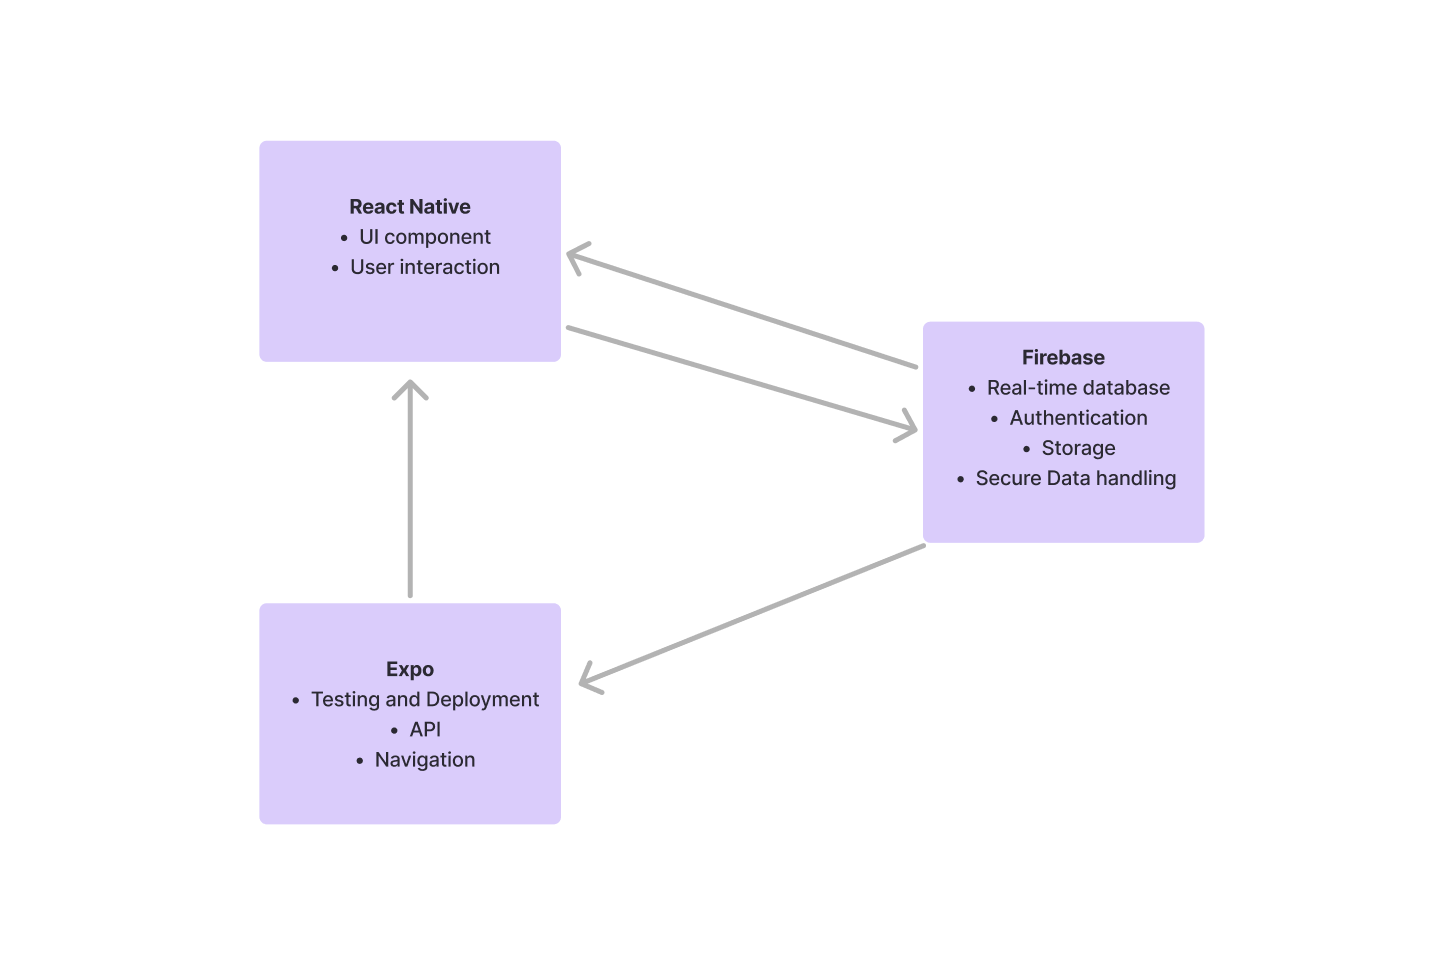
\includegraphics[width=1.2\linewidth]{exampleis-master/figures/Chapt3.3.png}
    \caption{The relationships between React Native, Expo, and Firebase, along with their respective roles in the app.}
    \label{fig:integration1}
\end{figure}

As shown in Figure \ref{fig:integration1}, React Native forms the core UI, providing a consistent user experience. It integrates with Expo for device-specific features like image selection and navigation, while Firebase manages real-time data, user authentication, and media storage. This streamlined workflow ensures secure, responsive, and cross-platform functionality.


\section{Supporting Libraries and Dependencies}
Several supporting libraries are included to handle essential functionalities and enhance the app’s user experience:

\begin{itemize}
     \item \textbf{Expo Router}: 
     The \texttt{expo-router} library plays a crucial role in managing navigation within the application. It enables structured and dynamic transitions between screens, ensuring that users can easily move through different parts of the app. For instance, we can see in Chapter \ref{chap:Chaptert5} , Listing \ref{lst:index} the navigation between the \texttt{LoginScreen} and \texttt{HomeScreen} is dynamically managed based on the user’s authentication status. This approach allows the app to direct users to appropriate screens without manual intervention, maintaining a coherent flow throughout the application. The use of \texttt{expo-router} eliminates the complexity of handling navigation manually, allowing for organized routing that responds automatically to user interactions and authentication changes.

    \item \textbf{Firebase SDK}: The \textbf{Firebase Software Development Kit (SDK)} is a core dependency, providing direct access to essential services discussed in Section \ref{sec:coredev} like Firestore, Authentication, and Storage services.
    The following code snippet in Listing \ref{lst:firebase_setup} demonstrates the Firebase setup used in the project. It outlines the configuration required to initialize Firestore, Authentication, and Storage services, ensuring proper data management and secure user access across the app\cite{firebasecookbook}.

\end{itemize}
\begin{lstlisting}[caption={Firebase Setup}, label={lst:firebase_setup}, numbers=left,stepnumber=1, numberstyle=\tiny\color{gray}]
import { initializeApp } from "firebase/app";
import { getFirestore, getAuth, initializeAuth, getStorage } from "firebase";
import AsyncStorage from "@react-native-async-storage/async-storage";
const firebaseConfig = {
    apiKey: "YOUR_API_KEY",
    authDomain: "YOUR_PROJECT.firebaseapp.com",
    projectId: "YOUR_PROJECT",
    storageBucket: "YOUR_PROJECT.appspot.com",
    messagingSenderId: "YOUR_SENDER_ID",
    appId: "YOUR_APP_ID"
};
const app = initializeApp(firebaseConfig);
export const db = getFirestore(app);
export const auth = initializeAuth(app, { persistence: getReactNativePersistence(AsyncStorage) });
export const storage = getStorage(app);
\end{lstlisting}


Following the Firebase setup shown in Listing \ref{lst:firebase_setup}, it is essential to break down the code to provide a clear understanding of how Firebase services are integrated into the application. Each part of the code plays a crucial role in ensuring that user data, authentication, and media storage are managed effectively.

The first three lines import the necessary modules required to access Firebase services. The \textbf{initializeApp} function from  \textbf{Line 15} is used to initialize the Firebase application with the configuration settings provided via lines  \textbf{Lines6-12}. The functions \textbf{getFirestore}, \textbf{getAuth}, \textbf{initializeAuth}, and \textbf{getStorage} provide access to Firebase's key services. \textbf{AsyncStorage} is imported to ensure user authentication sessions persist even after the app is closed, enhancing user convenience.

 \textbf{Line6-13} it defines the Firebase configuration object, which contains unique identifiers and keys that connect the app to the specific Firebase project. Each key serves a distinct purpose:
\begin{itemize}
\item \textbf{apiKey} authenticates requests from the app to Firebase services.
\item \textbf{authDomain} specifies the domain used for authentication processes.
\item \textbf{projectId} identifies the Firebase project associated with the app.
\item \textbf{storageBucket} refers to the cloud storage location where user images are stored.
\item \textbf{messagingSenderId and appId} helps manage notifications and application identification.
\end{itemize}

In the final part of the setup, (\textbf{lines 15-18})Firebase services are initialized:

\begin{itemize}
\item \textbf{initializeApp(firebaseConfig)} activates Firebase within the application using the previously defined configuration.
\item \textbf {getFirestore(app)} initializes Firestore, which stores user wardrobe data, including item details and metadata.
\item \textbf {initializeAuth(app, {persistence: getReactNativePersistence(AsyncStorage) })} initializes Firebase Authentication. The persistence setting ensures that the user's login session is remembered, so they remain logged in even after closing the app.
\item \textbf {getStorage(app)} sets up Firebase Storage, which securely stores user-uploaded clothing images. These images are linked to user profiles and can be accessed across devices.
\end{itemize}

\section{Development Configurations}
To ensure consistency and compatibility across different development environments, specific configurations are established. These configurations not only support efficient development but also safeguard sensitive information and optimize the app's performance across multiple platforms.

\textbf{The Node Package Manager (npm)} plays a central role in managing the application’s dependencies. Node.js, in version 16.x, was selected due to its compatibility with the core libraries used in the project. The \texttt{package.json} file outlines all dependencies along with their specific versions. This setup ensures that developers working on the project can initialize identical environments, preventing issues related to mismatched library versions. By maintaining consistency in the development environment, the risk of integration errors is minimized, and collaborative work becomes more efficient \cite{nodeessentials} \cite{nodecompleteguide}.
Managing sensitive information, such as Firebase API keys and configuration settings, was addressed through the use of environment variables. These variables are stored in \texttt{.env} files, which are excluded from version control to prevent unauthorized access. This approach ensures that sensitive data remains secure while still being accessible during development. By separating configuration data from the core codebase, the application remains flexible, allowing for easy modifications to environment-specific settings without altering the main code.

Another critical aspect of the development configuration involves platform-specific testing and debugging. The \textbf{Expo CLI} provides tools for testing the application across various devices and platforms. Commands like \texttt{expo start} enable real-time testing on both physical devices and emulators, facilitating the identification and resolution of platform-specific issues. This testing strategy is particularly important for features such as image uploads and gesture-based navigation, which can behave differently on iOS and Android. Ensuring compatibility across these platforms improves the reliability of the application and provides a consistent user experience.


\section{Summary of Development Tools}
The development tools and configurations described in this chapter form the backbone of My Digital Wardrobe. The use of \textbf{ React Native} and \textbf{Expo} ensures a uniform user interface and responsive performance across iOS and Android devices \cite{reactnative}. \textbf{Firebase} provides robust backend support, managing data storage, authentication, and media handling in a secure and scalable manner. Additionally, the development configurations, including consistent package management, secure handling of environment variables, and comprehensive platform testing, contribute to a stable and adaptable development process\cite{reactfirebase} \cite{firebasecookbook}.

With this structured environment in place, the subsequent chapter, Chapter \ref{chap:Chapter4} will provide an in-depth exploration of the system architecture of \textit{ My Digital Wardrobe}. It will examine how the selected tools and configurations support the application's core components, including navigation flows, real-time data management, and media storage integration. The discussion will highlight how each element contributes to the overall performance, scalability, and user experience of the application.



%!TEX root = ../username.tex
\lstset{
    backgroundcolor=\color{white},
    basicstyle=\footnotesize\ttfamily,
    breaklines=true,
    frame=single,
    captionpos=b,
    numbers=left,
    numberstyle=\tiny\color{gray},
    keywordstyle=\color{blue},
    commentstyle=\color{green},
    stringstyle=\color{red}
}
\chapter{Architecture of My Digital Wardrobe}
\label{chap:Chapter4}

{Integration of Different System Architecture}
In this Chapter we will discuss the different Architectures that work together to develop this application. 
 The architecture of \textit{My Digital Wardrobe} combines two key systems:\textbf{Client-Server} and \textbf{React Native Architecture}. These systems work together to create a mobile application that allows users to easily manage their wardrobes, upload images, and create outfit combinations. The frontend allows users to interact with the app smoothly, while Firebase manages data storage, authentication, and images. This setup lets users access their wardrobe from any device.
 

\section{The Client-Server Architecture}

The \textbf{Client-Server Architecture } 
describes how two main parts of the application—the \textbf{client} and the \textbf{server} —communicate with each other to make the app function smoothly.

\noindent \textbf{Understanding the Client and Server Roles}:
\begin{itemize}
    \item \textbf{Client (Frontend)}: The client is the part of the app that users see and interact with on their mobile devices. In My Digital Wardrobe, the client is built using React Native and Expo, which means the app looks and feels like a native mobile app on both iOS and Android. When users perform actions such as uploading a clothing image, browsing wardrobe items, or creating an outfit, the client sends these requests to the server.
    \item \textbf{Server (Backend)}: The server is like the "brain" behind the app, handling data processing and storage. In this app, Firebase acts as the server. It manages tasks such as storing user-uploaded images, saving wardrobe information, and authenticating users during login. Firebase also ensures that users’ data is securely stored and accessible only to them.
    
\end{itemize}

\noindent \textbf{How the Client and Server Work Together}:

When a user uploads a picture of a clothing item, the client (app on the phone) sends this image to Firebase (server). Firebase stores the image and sends back a confirmation that the upload was successful. The app then displays this image in the user’s wardrobe. This process happens in real-time, meaning that as soon as the server processes the data, the client updates the user interface accordingly.

This interaction allows the app to perform complex tasks like image storage and data management without slowing down the user’s phone. The heavy processing is done on Firebase’s servers, while the user enjoys a fast and responsive experience on their device.

\begin{figure}[h]
    \centering
    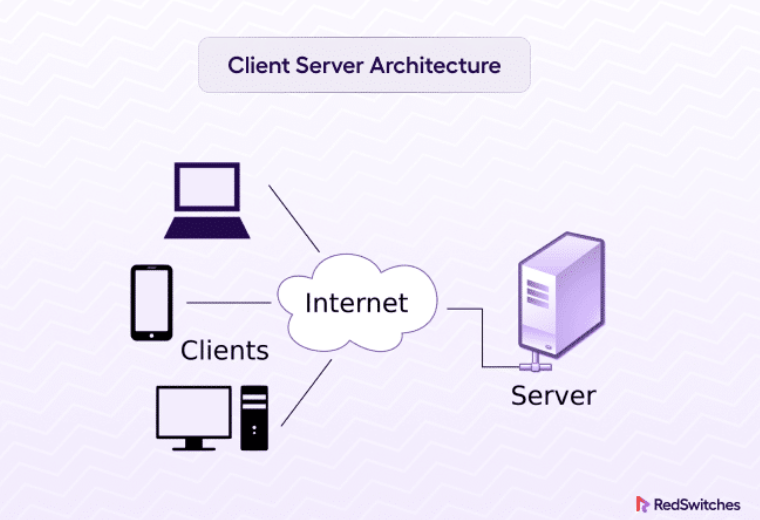
\includegraphics[width=0.9\linewidth]{exampleis-master/figures/C-S.png}
    \caption{The Client-Server architecture \cite{client_server_arch}}
    \label{fig:client_server_architecture}
\end{figure}

In Figure \ref{fig:client_server_architecture}, we can see that the client and server communicate continuously.
This client-server relationship ensures that the app remains lightweight on the client side while utilizing Firebase’s robust backend services for heavy-lifting operations such as storage and authentication\cite{client_server_arch}.

\section{React Native + Expo Architecture}

The frontend utilizes the \textbf{React Native + Expo Architecture}, enabling cross-platform compatibility while consisting  a modular and maintainable codebase. In simple terms, this architecture allows the app to work smoothly on both iOS and Android devices without the need to create two separate versions.
\textbf{React Native}, as discussed in the previous chapter(Chapter \ref{chap:Chaptert3}), enables the development of mobile applications using a single codebase across differnet devices. This ensures consistency across platforms while reducing development time and effort.

\textbf{Expo} complements React Native by providing tools and libraries that streamline common development tasks. It simplifies access to device-specific features such as the camera, image gallery, and navigation, eliminating the need for additional native code and accelerating the development process.

As seen in Figure \ref{fig:react_native_architecture} React Native's architecture revolves around the \textbf{Bridge Model}, which facilitates communication between the JavaScript logic and the Native components of the app \cite{react_native_arch}. Expo further enhances this framework by providing pre-built libraries and access to device-specific features, streamlining the development and deployment process.


\noindent \textbf{The main three features of React Native + Expo Architecture are }:
\begin{enumerate}
    \item \textbf{Declarative UI Design}: React Native allows us to describe what the app should look like, and it automatically updates the screen when the app’s data changes. This makes the user experience smoother, as the app responds immediately to user actions.
    \item \textbf{Cross-Platform Compatibility}: The architecture ensures that the app works the same way different devices without having to build two separate apps.
    \item \textbf{Expo's Prebuilt Libraries}: Expo simplifies development by offering APIs for native functionalities such as the camera, image picker, and navigation, eliminating the need for custom native modules in most scenarios.
\end{enumerate}
Next, we explain how the components in the Figure \ref{fig:react_native_architecture} work together in our app.
The React Native + Expo Architecture relies on a layered structure where each part has a specific job:
\begin{enumerate}

    \item\textbf{React Layer (User Interface and Logic)}:
This is the layer where developers write the code that defines how the app looks and behaves. For example, when users browse their wardrobe or select outfits, this layer controls what they see on the screen and how they interact with it.

    \item \textbf{JavaScript Thread (The Brain of the App)}:
This layer runs the JavaScript code that powers the app’s logic. It manages user interactions, such as tapping buttons or selecting images, and decides what should happen next.

    \item \textbf{Bridge Layer (The Translator)}:
The Bridge acts as a translator between the JavaScript code and the device’s native features. Since mobile devices run on native code, the bridge ensures that commands written in JavaScript are correctly understood by the phone’s operating system. For instance, when a user selects an image to upload, the bridge translates this action so the phone can access the image from the gallery.

    \item \textbf{Native Layer (Device-Specific Features)}:
This is where the app connects with the device’s built-in functions, such as the camera, storage, or touch gestures. It ensures that animations run smoothly, images load quickly, and user interactions feel natural and responsive.
\end{enumerate}


\begin{figure}[h]
    \centering
    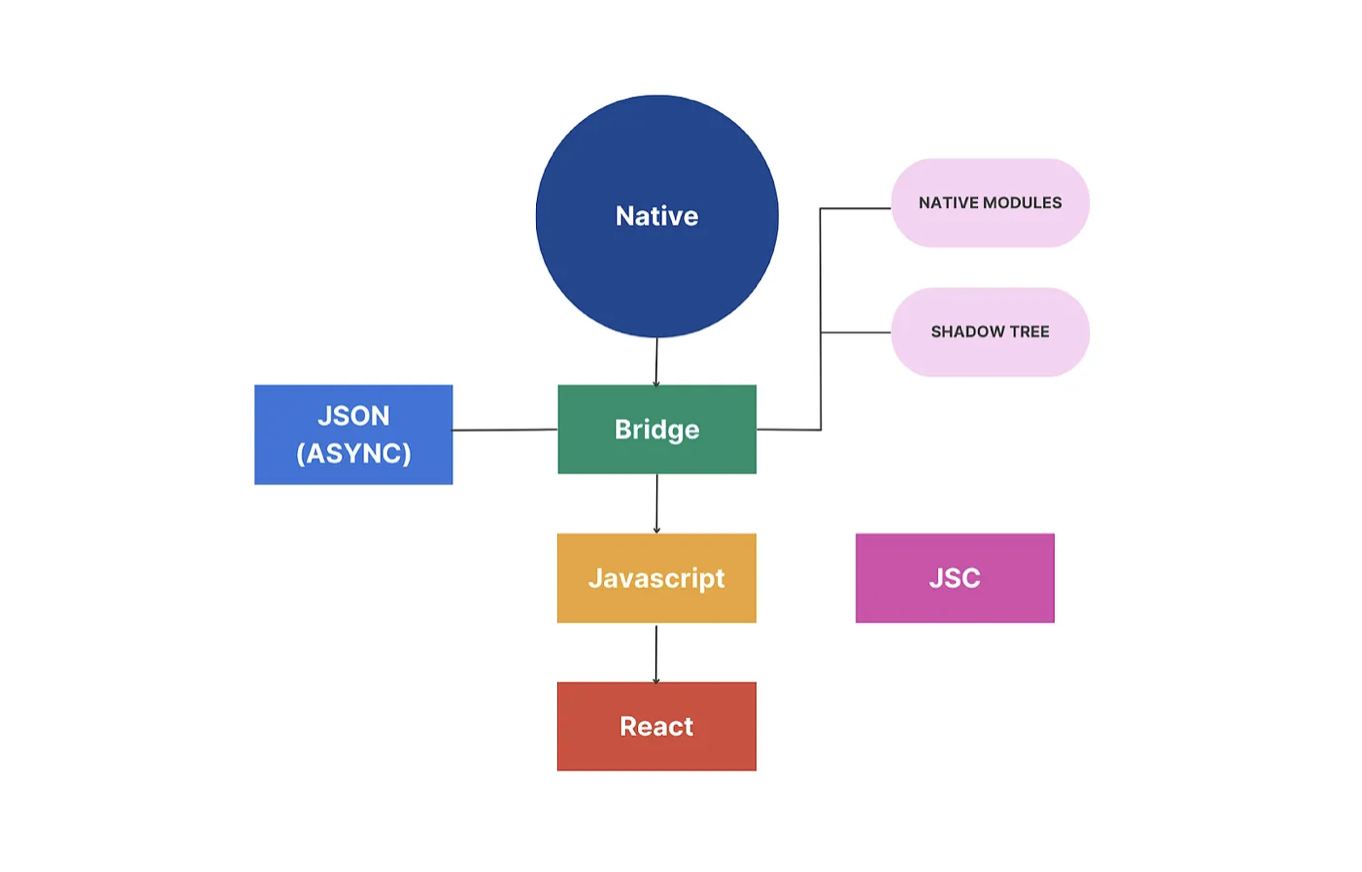
\includegraphics[width=0.8\linewidth]{exampleis-master/figures/ReactNative.png}
    \caption{The React Native  architecture \cite{react_native_arch} }
    \label{fig:react_native_architecture}
\end{figure}


Next, to better understand how this architecture functions, lets consider the process of a user uploading an image of a clothing item in \textbf{ My Digital Wardrobe}:

\begin{itemize}
    \item \textbf{Step 1: User Action }A user uploads an image.
    \item \textbf{Step 2: React Layer Response }The React layer triggers Expo’s ImagePicker API, which opens the device’s gallery.
    \item \textbf{Step 3: Bridge in Action }The bridge translates this request from JavaScript into a command the phone understands, allowing access to the gallery.
    \item \textbf{Step 4: Native Layer Processing }The user selects an image, and the native layer retrieves it from the phone’s storage.
    \item \textbf{Step 5: Data Sent Back }The image is sent back through the bridge to the JavaScript layer for further processing such as resizing or preview rendering can occur.
    \item \textbf{Step 6: Storage in Firebase }Finally, the image is uploaded to Firebase, where it is stored securely and displayed in the user’s digital wardrobe ready for viewing, editing, or mixing and matching with other clothing items.
    
\end{itemize}


This architecture ensures that the app benefits from React Native's flexibility for building responsive, modular components while utilizing Expo's tools to handle platform-specific integrations. By utilizing the Bridge model, \textit{My Digital Wardrobe} achieves a balance between cross-platform efficiency and near-native performance.

\section{Backend and Data Storage}

Firebase serves as the \textit{Backend-as-a-Service (BaaS)} for \textit{My Digital Wardrobe}, streamlining backend management and providing powerful features such as \textbf{real-time data synchronization}, \textbf{secure cloud storage}, and \textbf{user authentication}. This architecture eliminates the need for dedicated servers, allowing the app to directly interact with Firebase services via its SDKs, ensuring scalability and ease of integration \cite{firebase_intro}.

\begin{figure}[h]
    \centering
    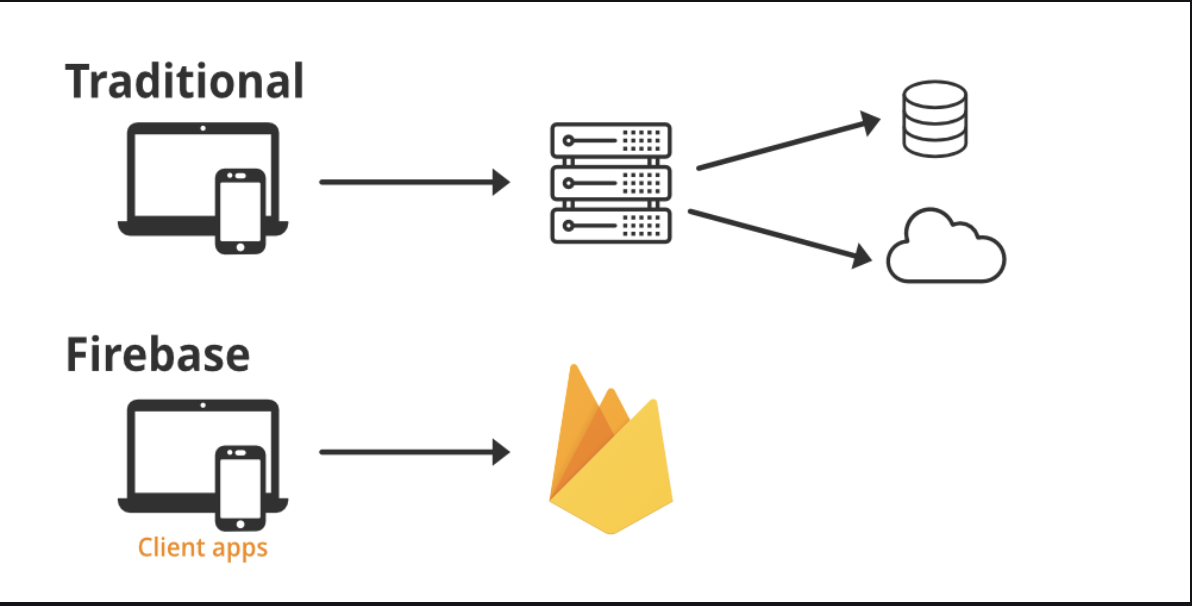
\includegraphics[width=0.6\linewidth]{exampleis-master/figures/firebase.png}
    \caption{Firebase as a Backend-as-a-Service\cite{firebase_intro}}
    \label{fig:firebase_backend}
\end{figure}

\subsection{Traditional Databases vs. Firebase (Firestore)}

To understand why Firebase is ideal for My Digital Wardrobe, it’s helpful to compare it with a traditional database.
\begin{itemize}
    \item \textbf{Traditional Databases:}
These databases, such as\textbf{ MySQL} or \textbf{PostgreSQL}, store data in tables with rows and columns, similar to a spreadsheet. To access or update data, applications typically need a separate server that handles communication between the app and the database (see Figure \ref{fig:firebase_backend}. For example, when a user uploads an image, the request first goes to the server, which then stores the image in the database and sends a response back. While this approach is reliable, it can be slower and more complex, especially when handling real-time updates across multiple users.

\item \textbf{Firebase Firestore (NoSQL Database):}
In contrast, Firestore—the database used by Firebase—stores data in a more flexible structure using collections and documents, similar to a filing cabinet with labeled folders. For My Digital Wardrobe, one collection might store wardrobe items, while another stores outfit combinations. Each document in a collection contains key-value pairs, making it easy to store diverse data like image URLs, categories, and timestamps.
Unlike traditional databases, Firestore allows the app to communicate directly with the database, eliminating the need for a separate server. This direct connection ensures real-time synchronization, meaning any changes users make (like uploading a new clothing item) are instantly visible in the app without refreshing or waiting.
\end{itemize}
\subsection{Firebase in My Digital Wardrobe}
In this section, we discuss how \textbf{Firebase} provides two core services that are essential for managing wardrobe data and images:
\begin{enumerate}
    \item \textbf{Cloude Storage for Images}
    When users upload photos of clothing items, these images are stored in Firebase Cloud Storage. Each image is given a unique web link (URL), allowing the app to retrieve and display it whenever needed. This process happens in the background, ensuring that images load quickly without slowing down the app.
    \item \textbf{Firestore Database for Organizing Wardrobe Items}
    The Firestore database organizes all user data related to clothing items and outfits. It keeps everything neatly structured, making it easy for users to browse, sort, and filter their wardrobe. Key information stored in Firestore includes:
   
    \begin{itemize}
        \item \textbf{Categories}: Classifications like tops, bottoms,  enabling easy filtering and browsing within the app.
        \item \textbf{File Names}: Unique identifiers for each uploaded image, generated with timestamps and random identifiers to ensure no file overwriting occurs.
        \item \textbf{Image URLs}: Direct links to the images stored in Firebase Cloud Storage, used to retrieve and display the images in the app’s interface.
        \item \textbf{Timestamps}: Date and time of upload, which can be used to organize and sort wardrobe items chronologically.
    \end{itemize}
\end{enumerate}


The Firestore database serves as the backbone for data management in the application. As illustrated in Figure \ref{fig:firestore_collections}, the database structure is designed to support two key functionalities: managing individual wardrobe items and storing outfit combinations. 
\begin{enumerate}
    \item \textbf{Wardrobe Items:} Storing individual clothing pieces with relevant details like category and image location.
    \item \textbf{Outfit Items:} Saving user-created outfits by linking selected wardrobe items together, allowing users to revisit and reuse their favorite combinations.
\end{enumerate}

\begin{figure}[!ht]\centering
    % First Subfloat: Wardrobe Items
    \subfloat[Firestore structure for wardrobe items.][Wardrobe Items]
    {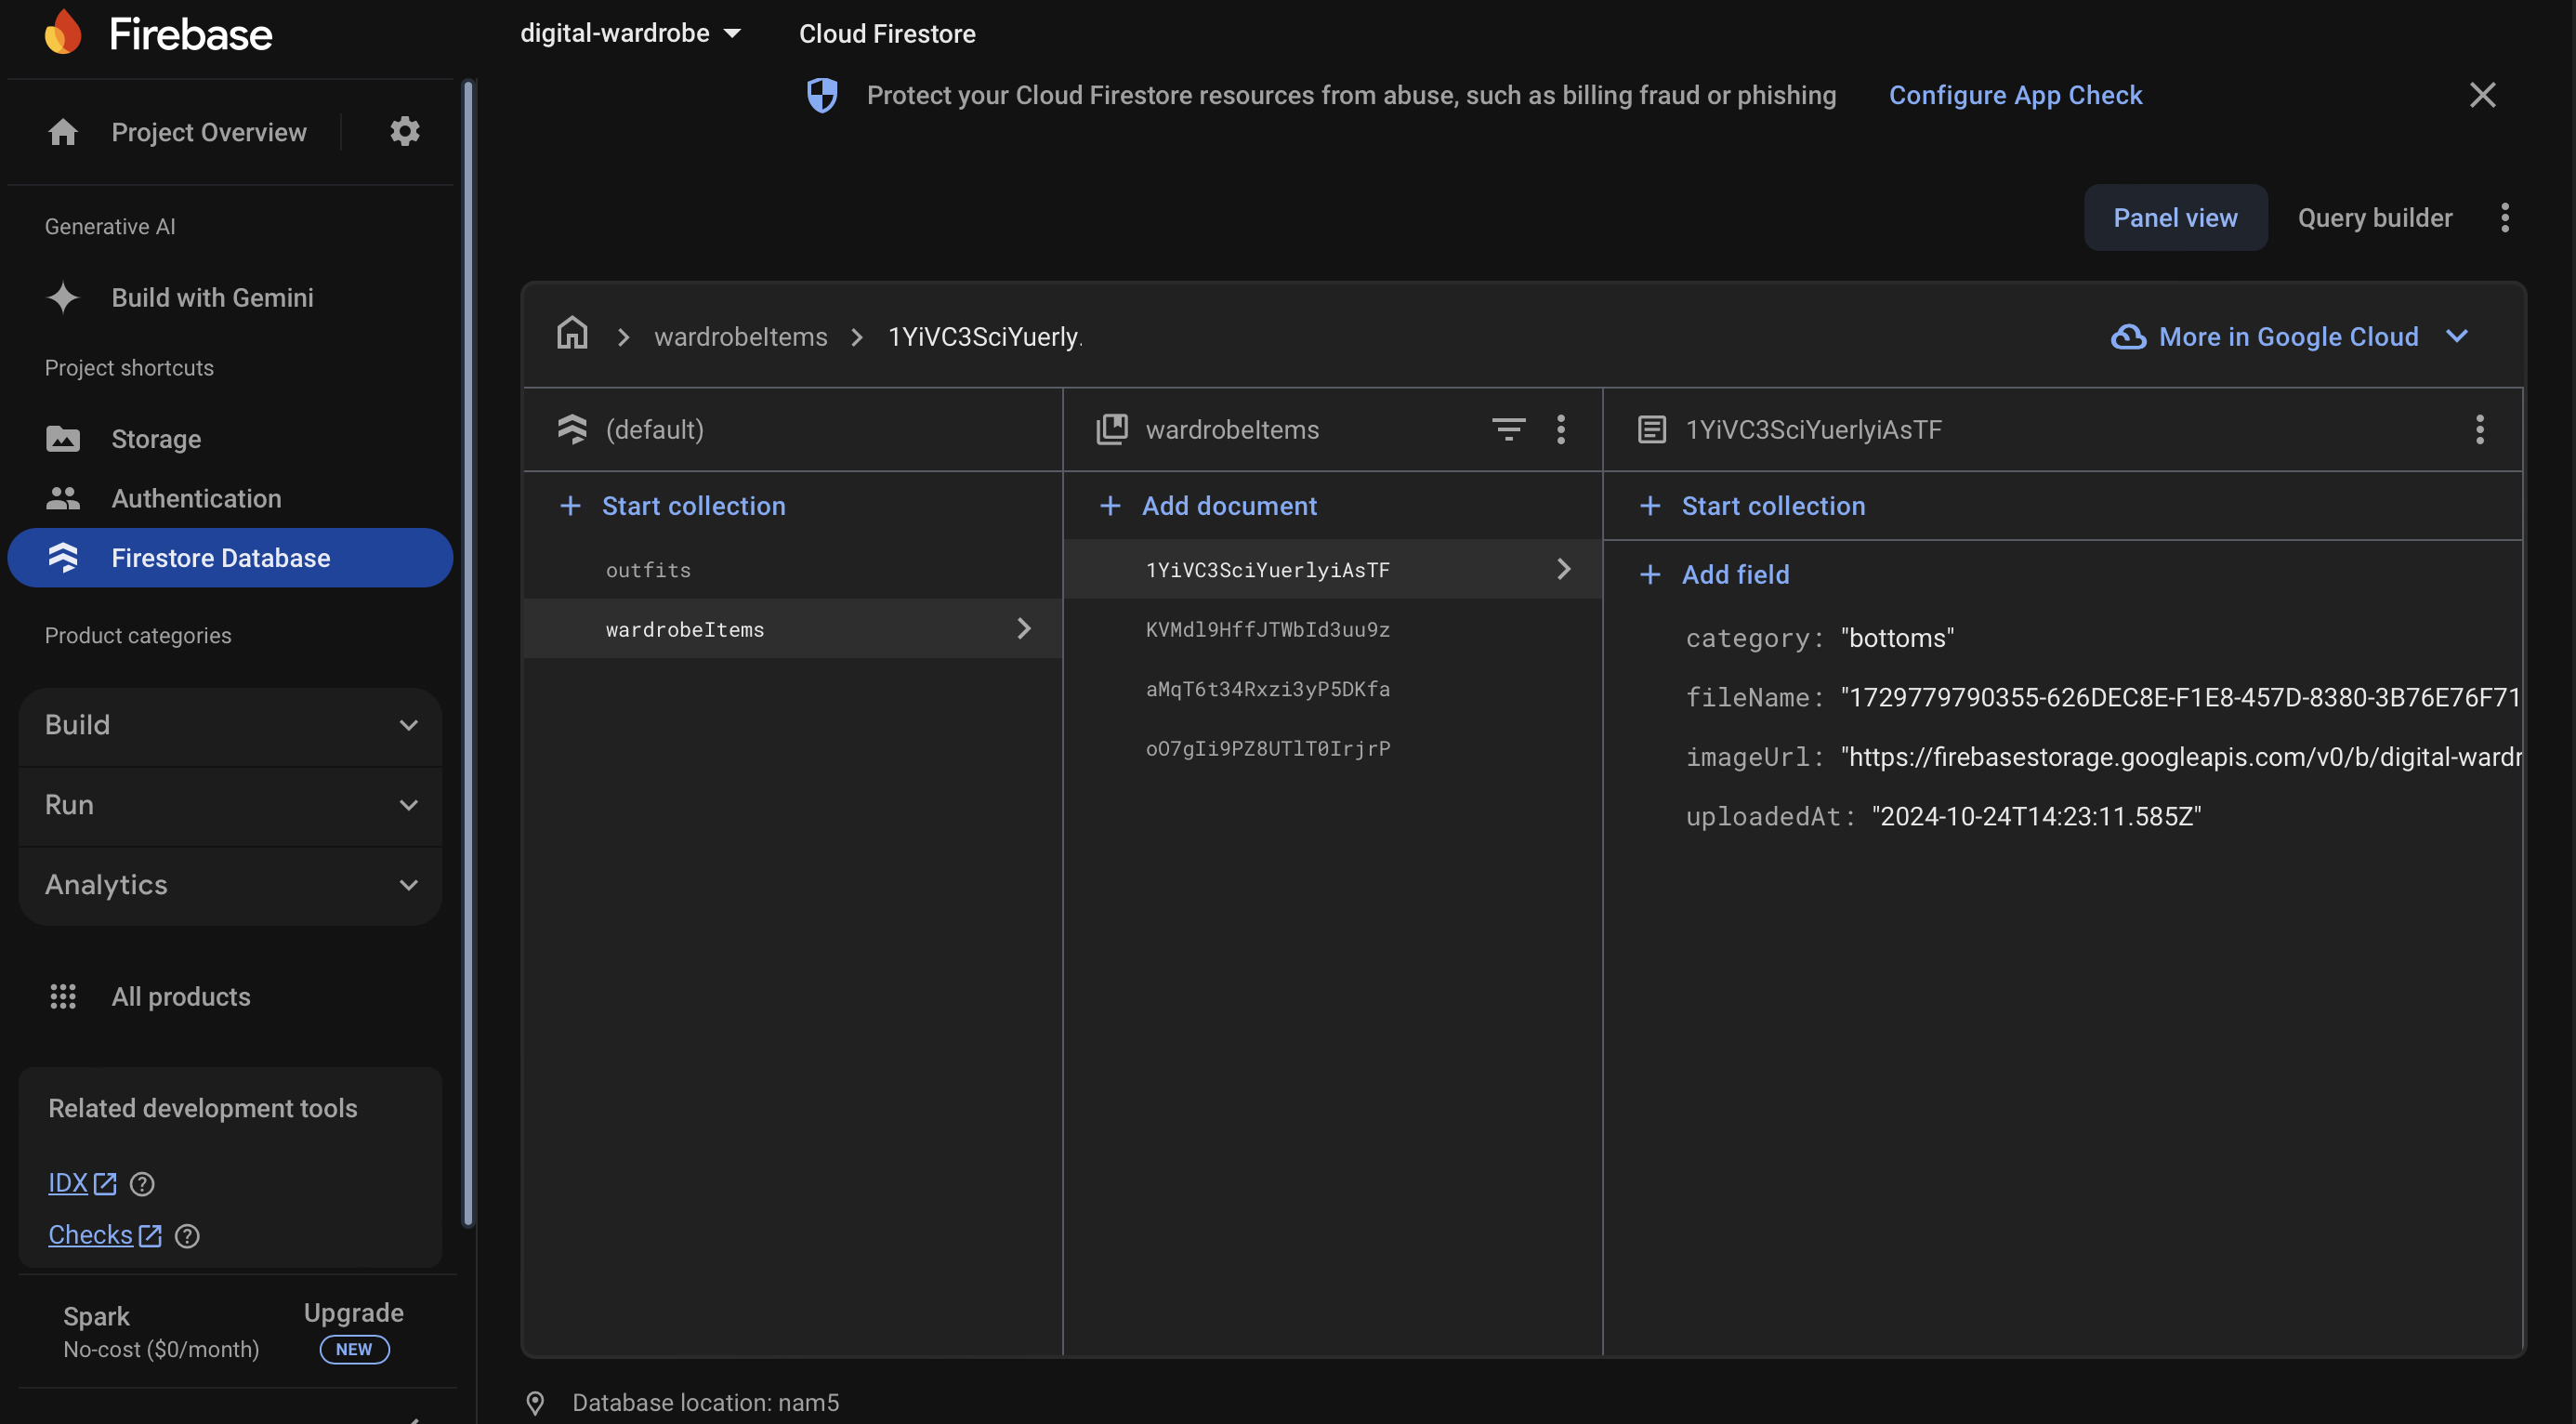
\includegraphics[width=0.8\textwidth]{exampleis-master/figures/wardrobeitemFB.png}\label{fig:wardrobe_items}}
    \qquad % Adds horizontal spacing between the images
    % Second Subfloat: Outfit Items
    \subfloat[Firestore structure for outfit combinations.][Outfit Items]
    {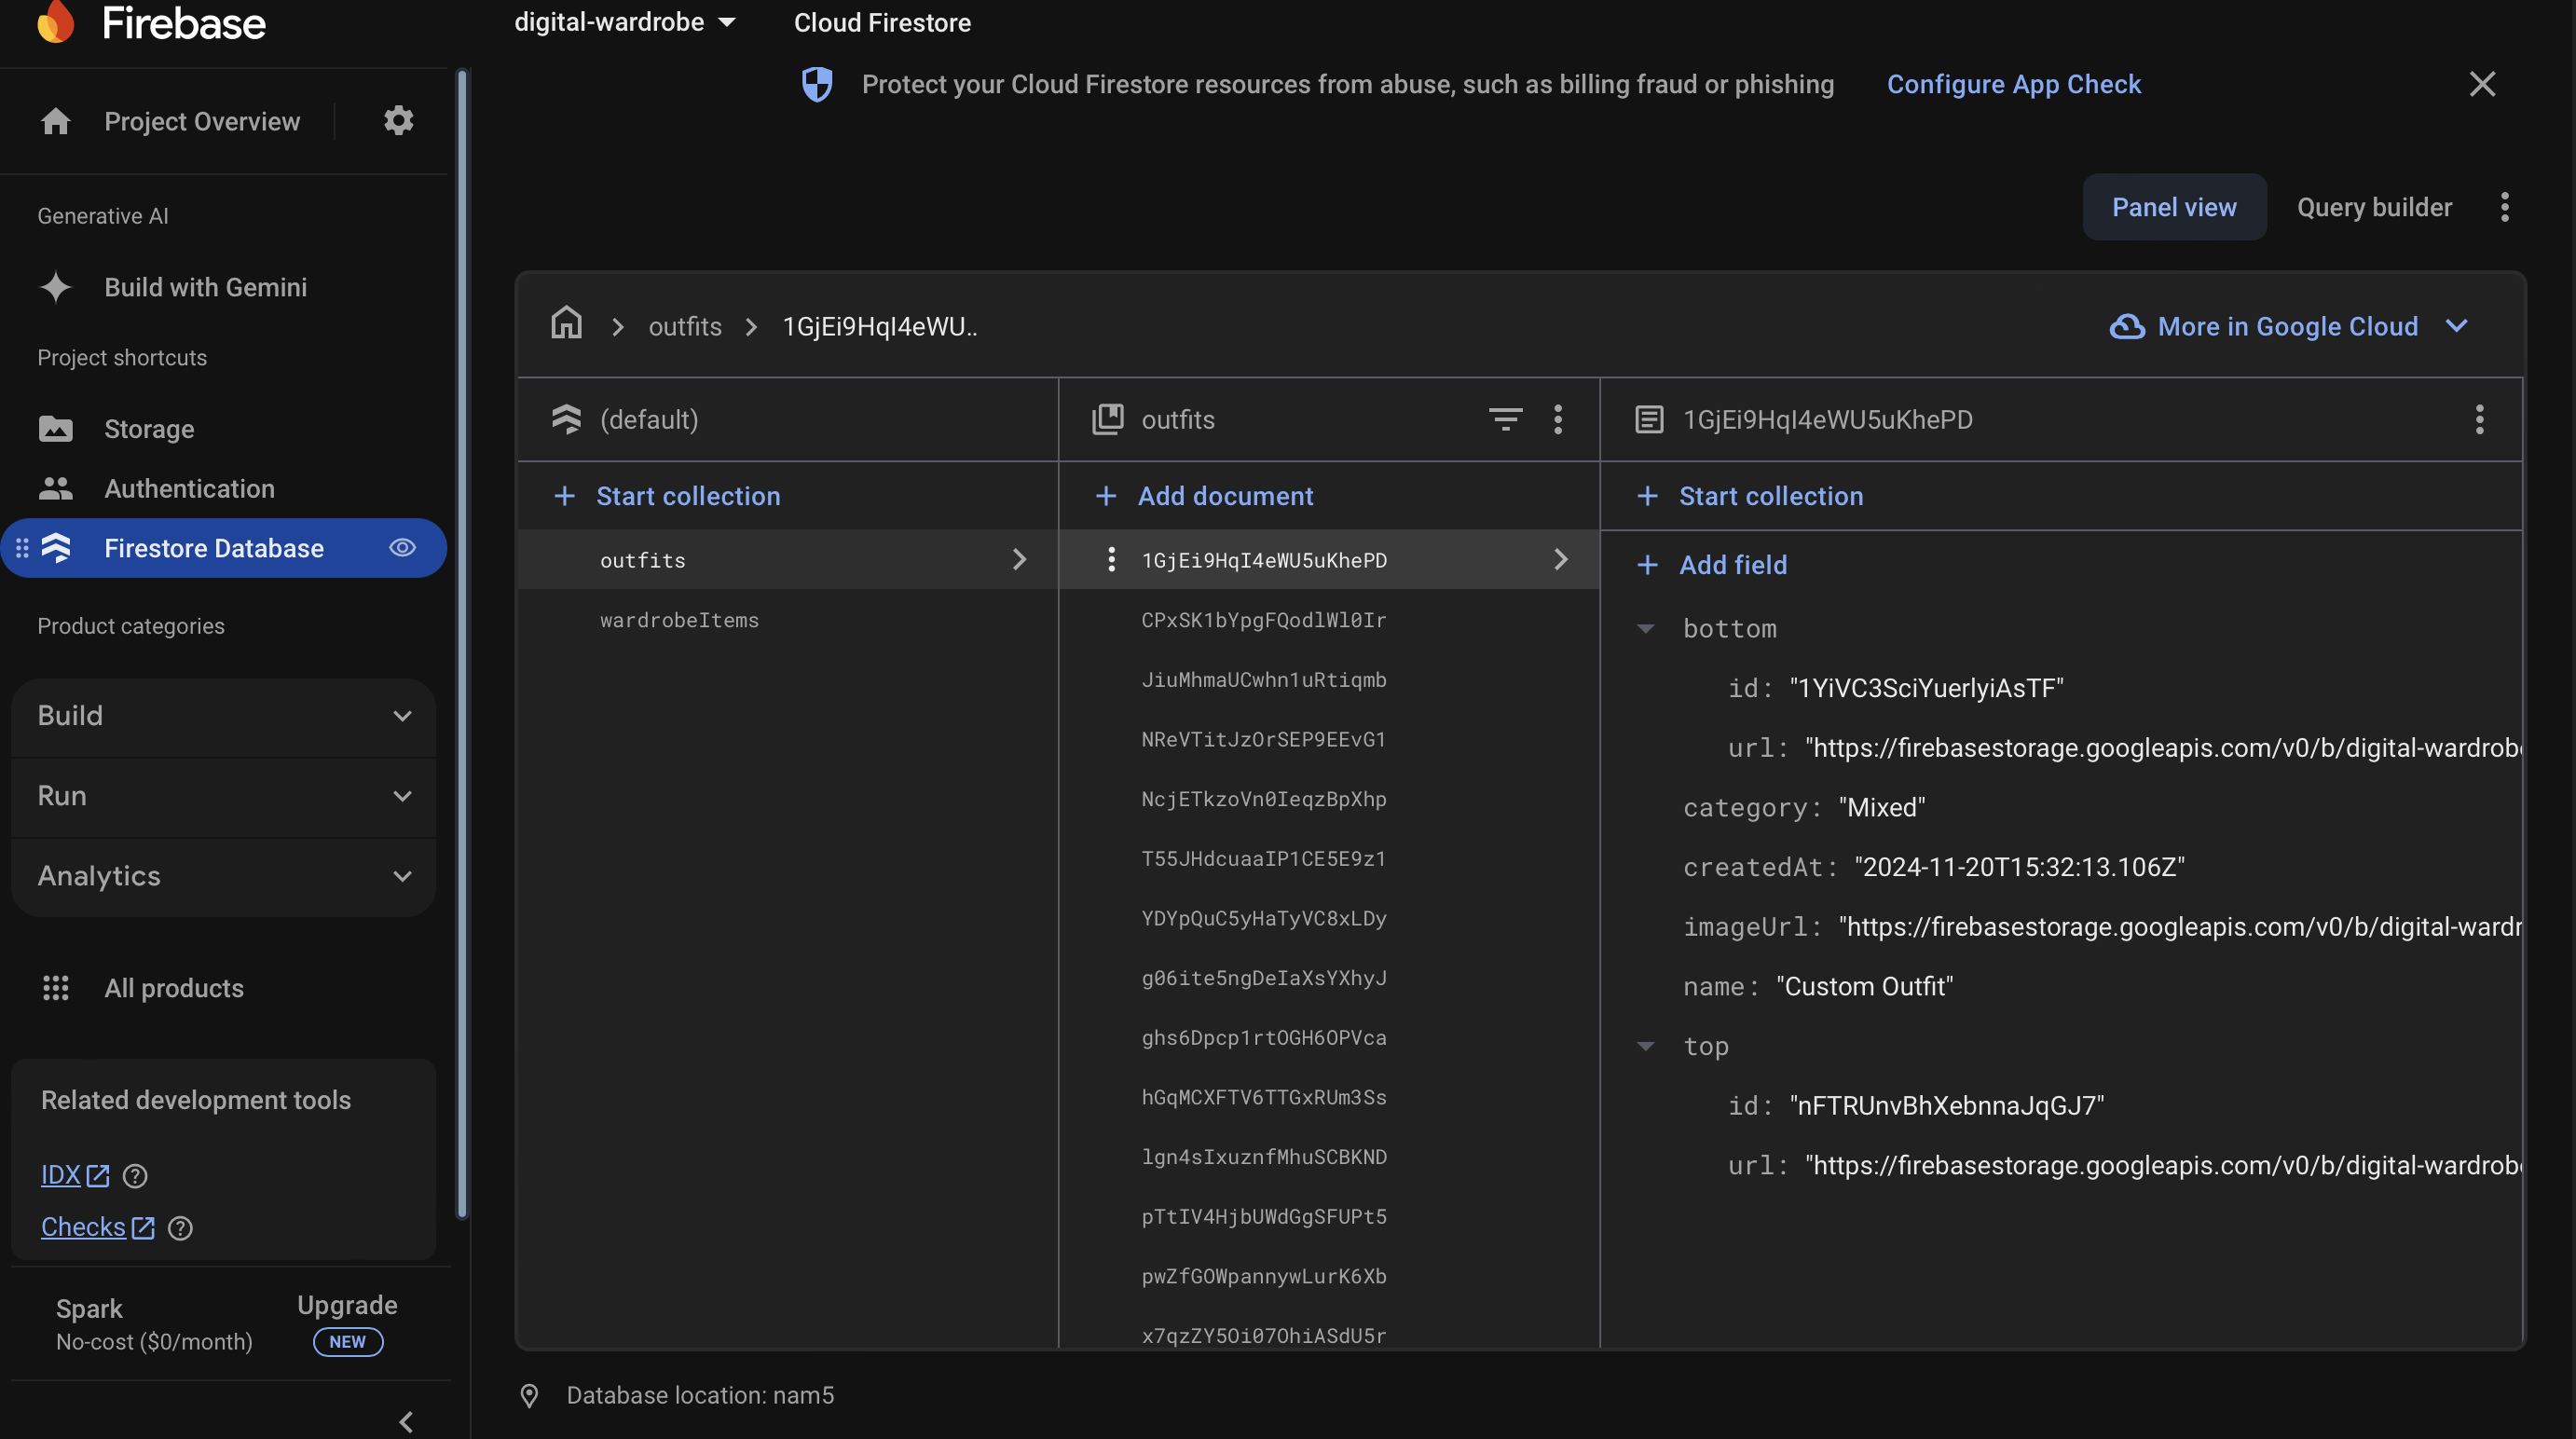
\includegraphics[width=0.8\textwidth]{exampleis-master/figures/OutfititemFB.png}\label{fig:outfit_items}}
    \caption{Firestore collections for wardrobe items and outfits.}
    \label{fig:firestore_collections}
\end{figure}


The integration of Firebase Cloud Storage and Firestore \textit{My Digital Wardrobe}provides a smooth and reliable experience, where users can easily organize and experiment with their wardrobe collections.

\section{Authentication and Security}

For \textit{My Digital Wardrobe}, ensuring that user data remains safe and accessible only to the right person is important. This is where authentication and security come into play. Think of authentication as the app's way of checking, "Who are you?" and security as the process of making sure that only the right people can see or change certain information.

Authentication in \textit{My Digital Wardrobe} is handled by \textbf{Firebase Authentication}, which allows users to sign in securely. Instead of building complicated login systems from scratch, Firebase provides easy-to-use tools for this purpose. Users can log in with an email and password or even through trusted services like Google or Facebook.

When a user logs in, Firebase creates a secure connection between the user and their personal wardrobe data. This ensures that only that user can view or edit their clothing items and outfits. It’s similar to how online banking systems require customers to log in before showing their account details—only they have access.


While authentication checks who they are, security rules decide what they can do. In My Digital Wardrobe, Firebase uses Firestore Security Rules to protect data. These rules ensure that each user can only see or change their wardrobe items, preventing unauthorized access.

For example, if two users use the app, User A cannot see or edit User B’s wardrobe. Firebase automatically checks who is making the request and allows or blocks access based on the security rules set for the app. This protects sensitive data and ensures privacy.

In Listing \ref{lst:firestore_rules} Firestore Security Rules enforce access policies for the database.

\begin{lstlisting}[caption={Firestore Security Rules}, label={lst:firestore_rules}]
rules_version = '2';
service cloud.firestore {
  match /databases/{database}/documents {
    match /{document=**} {
      allow read, write: if request.auth != null;
    }
  }
}
\end{lstlisting}

\noindent \textbf{Explanation of the Rules}:
\begin{itemize}
    \item \textbf{\texttt{rules\_version = '2'}}: Specifies the version of Firestore security rules being used.
    \item \textbf{\texttt{service cloud.firestore}}: Indicates the rules apply to Firestore, Firebase's NoSQL database service.
    \item \textbf{\texttt{match /databases/\{database\}/documents}}: Defines the scope of the rules, targeting all documents within the database.
    \item \textbf{\texttt{match /{document=**}}}: Includes all document paths, including nested sub-collections.
    \item \textbf{\texttt{allow read, write: if request.auth != null}}: Grants read and write permissions only to authenticated users (\texttt{request.auth != null} ensures that the request is made by a logged-in user).
\end{itemize}
In simple terms, this means that unless the user has been authenticated (logged in), they cannot access any data. These rules apply to all parts of the wardrobe, ensuring that no unauthorized person can view or change the information.

Beyond controlling who can access the data, My Digital Wardrobe uses encryption to protect information when it’s being transferred between the app and Firebase’s servers. Think of encryption as converting the data into a secret code while it’s moving, so no one can read it if they intercept it. Once the data reaches its destination, it is decoded back to its original form. This ensures that even when users upload images or log in from different networks, their data remains secure and protected from potential threats.

Without proper authentication and security measures, anyone could access, modify, or delete user data. For an app like My Digital Wardrobe, this could mean losing carefully organized wardrobe collections or exposing personal images to others. By using Firebase's authentication and security tools, the app ensures that:
\begin{itemize}
    \item Each user’s data remains private.
    \item Unauthorized users cannot gain access.
    \item All communication between the app and the backend is protected.
\end{itemize}
The combination of Firebase Authentication and Firestore Security Rules forms a strong system that builds trust and ensure that users can confidently manage their wardrobes, knowing that their data is secure.

With a robust architecture in place, the next chapter will explore how these technologies and systems were brought to life through practical development. It will detail the step-by-step process of building the app’s key features, from user interface design and navigation flows to image uploading and outfit creation. The chapter will also discuss design principles that guided the creation of an intuitive user experience.
%!TEX root = ../username.tex
% Add your package includes here
\chapter{Design and Implementation of My Digital Wardrobe App}
\label{chap:Chaptert5}
\section{App Development Framework}

The development of this application prioritizes ease of use and efficiency in managing wardrobe items. This chapter walks readers through how the app works, highlighting key features like logging in, uploading images, organizing clothing items, and creating outfits. Since readers may not have direct access to the app, this chapter aims to provide a complete picture of the user experience. It explains how different parts of the app work together behind the scenes. 
\begin{figure}[h]
    \centering
    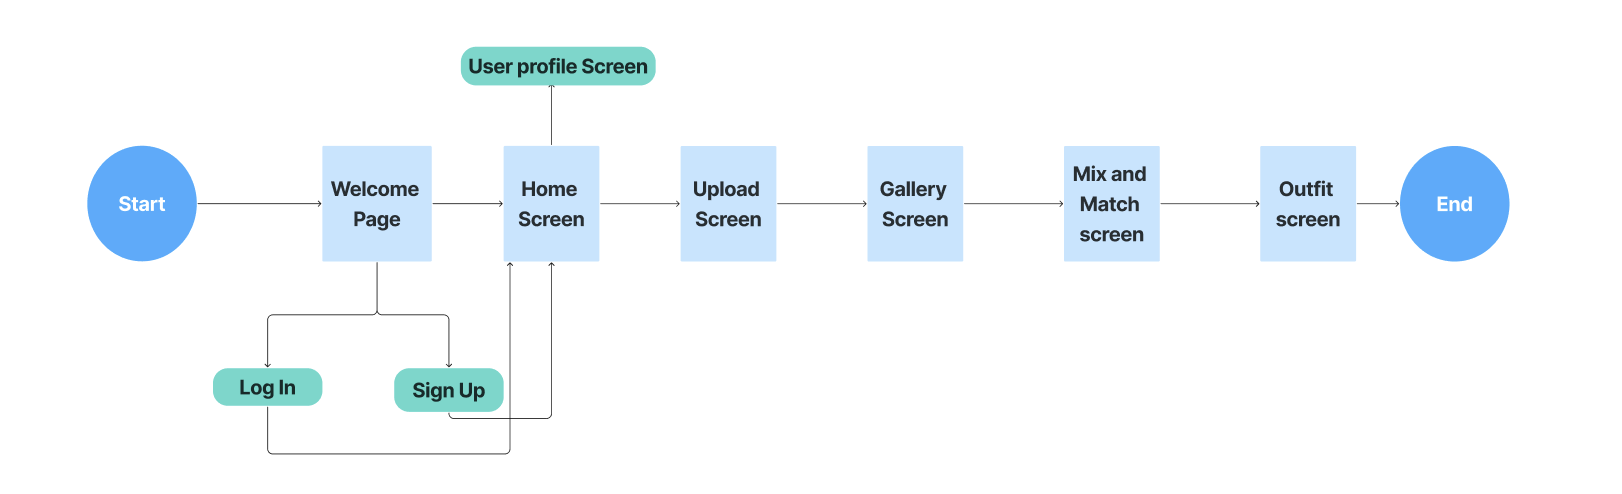
\includegraphics[width=1.1\linewidth]{exampleis-master/figures/updated workflow.png}
    \caption{Screen navigation}
    \label{fig:integration}
\end{figure}

\subsection{Workflow Overview}
The workflow of My Digital Wardrobe outlines how users interact with the app, from signing up to creating and saving outfits. Figure \ref{fig:integration} presents a simplified workflow demonstrating how new users navigate through the app, while  Figure \ref{fig:integration2}  provides a visual representation of this process, highlighting the relationship between user actions, navigation flows, and Firebase services that operate behind the scenes.

\begin{figure}[h]
    \centering
    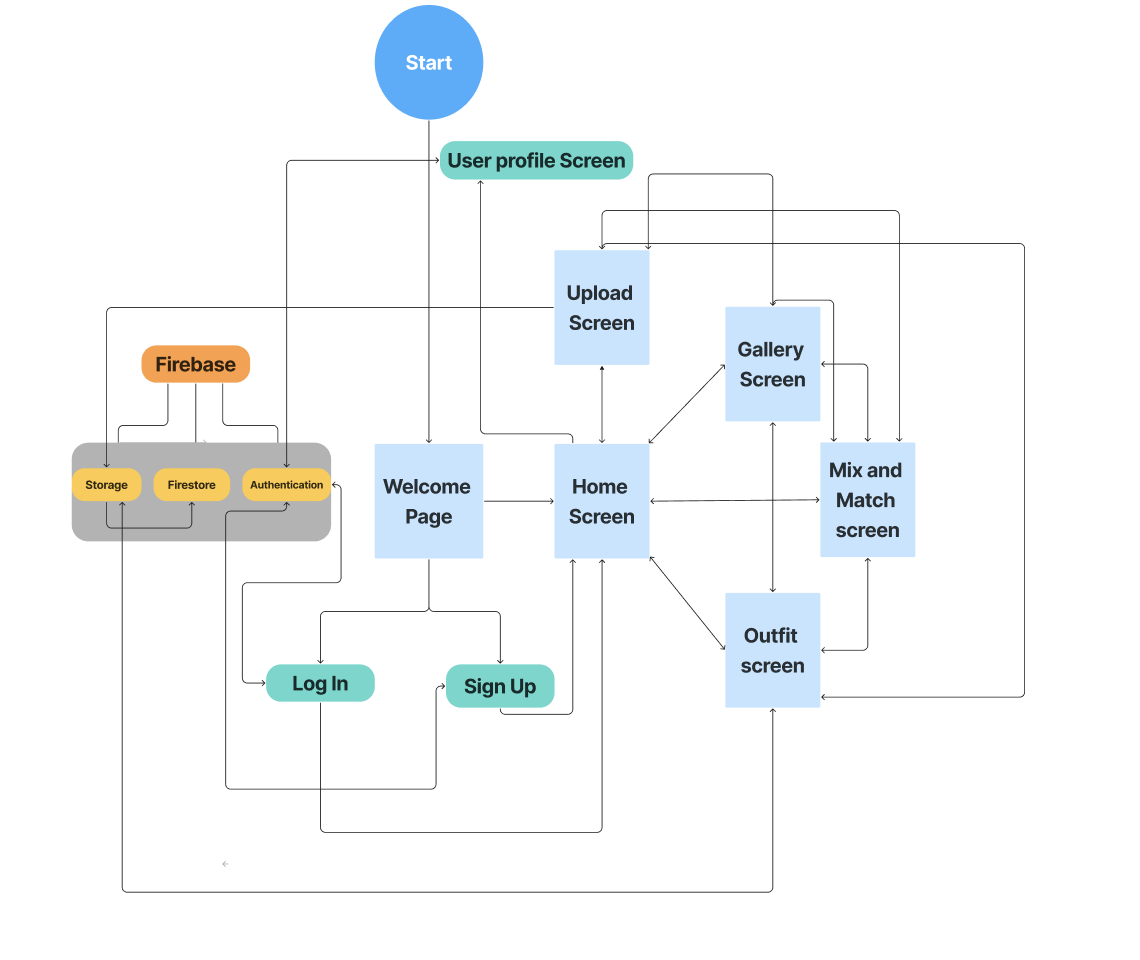
\includegraphics[width=1.0\linewidth]{exampleis-master/figures/updated diagram.png}
    \caption{Workflow diagram}
    \label{fig:integration2}
\end{figure}


At the core of the workflow is the integration between user interactions and backend processes. Users begin at the \textbf{Welcome Page}, where they can either  \textbf{log in} or  \textbf{sign up}. Successful authentication, managed by Firebase, directs users to the  \textbf{Home Screen}, which acts as the central hub. From here, users can navigate to various screens, including the  \textbf{Upload Screen} for adding new wardrobe items, the  \textbf{Gallery Screen} for browsing uploaded clothing, and the  \textbf{Mix and Match Screen}, where outfits can be created and later reviewed on the \textbf{ Outfit Screen}.

Firebase’s services support these interactions. As mentioned in Chapter \ref{chap:Chaptert3},  Authentication verifies user access, Storage handles image uploads, and Firestore organizes metadata for efficient retrieval and categorization. The User Profile Screen is accessible for managing personal information and preferences, ensuring a personalized experience throughout.
This structured workflow ensures that each user action leads to a logical next step, with Firebase managing data storage and access in the background. The navigation between screens is handled dynamically, providing a fluid and intuitive user experience. Further sections will explore each component of this workflow in greater detail, discussing how authentication, image handling, and gesture-based browsing are implemented to support the app’s core functionalities.

\subsection{Authentication and Security}
Authentication and navigation are managed using Firebase Authentication and Expo Router, working together to provide secure access and smooth user flow throughout the app. The authentication process ensures that only authorized users can access their personalized wardrobe, while dynamic navigation adapts to user actions in real time.
The core logic for authentication and routing is handled in the \textit{index.js} file, where Firebase continuously monitors user login status and directs users to the appropriate screen based on their authentication state. 
The following code snippet in Listing \ref{lst:index} shows how authentication and navigation are integrated:
\begin{lstlisting}[caption={Authentication and routing in \texttt{index.js}}, label={lst:index}]
import { useEffect, useState } from "react";
import { useRouter } from "expo-router";
import { auth } from "./firebase";
import { onAuthStateChanged } from "firebase/auth";

const Index = () => {
    const router = useRouter();
    const [loading, setLoading] = useState(true);
    const [user, setUser] = useState(null);

    useEffect(() => {
        const unsubscribe = onAuthStateChanged(auth, (user) => {
            setLoading(false);
            setUser(user);
            if (user) {
                router.replace("/Screens/HomeScreen", { user });
            } else {
                router.replace("/Screens/LoginScreen");
            }
        });
        return () => unsubscribe();
    }, [router]);

    if (loading) {
        return <LoadingIndicator />;
    }

    return null;
};

export default Index;
\end{lstlisting}

The implementation ensures that users are directed to the appropriate screen based on their login status, providing both secure access and a smooth navigation experience.

The process begins by importing necessary dependencies \textbf{(Lines 1–4)}, including React’s \texttt{useEffect} and \texttt{useState} for managing component state and lifecycle, Expo Router’s \texttt{useRouter} for handling navigation between screens, and Firebase’s authentication tools (\texttt{auth} and \texttt{onAuthStateChanged}) to track user sessions.

The core functionality is encapsulated within the \texttt{Index} component \textbf{(Line 6)}. Inside this component, the router is initialized \textbf{(Line 7)} to control screen transitions, while two state variables—\texttt{loading} and \texttt{user} \textbf{(Lines 8–9)}—track the authentication process. The \texttt{loading} state ensures that a loading indicator is displayed while Firebase checks the user’s login status, preventing any unintended flashes of incorrect screens.

The \texttt{useEffect} hook \textbf{(Line 11)} plays a crucial role in this setup. It runs as soon as the component is mounted, triggering the \texttt{onAuthStateChanged} function \textbf{(Line 12)}. This function monitors authentication status in real time. If the user is authenticated \textbf{(Line 15)}, their information is stored in the \texttt{user} state \textbf{(Line 14)}, and they are redirected to the Home Screen using \texttt{router.replace()} \textbf{(Line 16)} as shown in Figure \ref{fig:home}. 

\begin{figure}[!ht]
    \centering
    % First Subfloat: Login Screen
    \subfloat[Login screen - entry point for user authentication.\label{fig:login}]
    {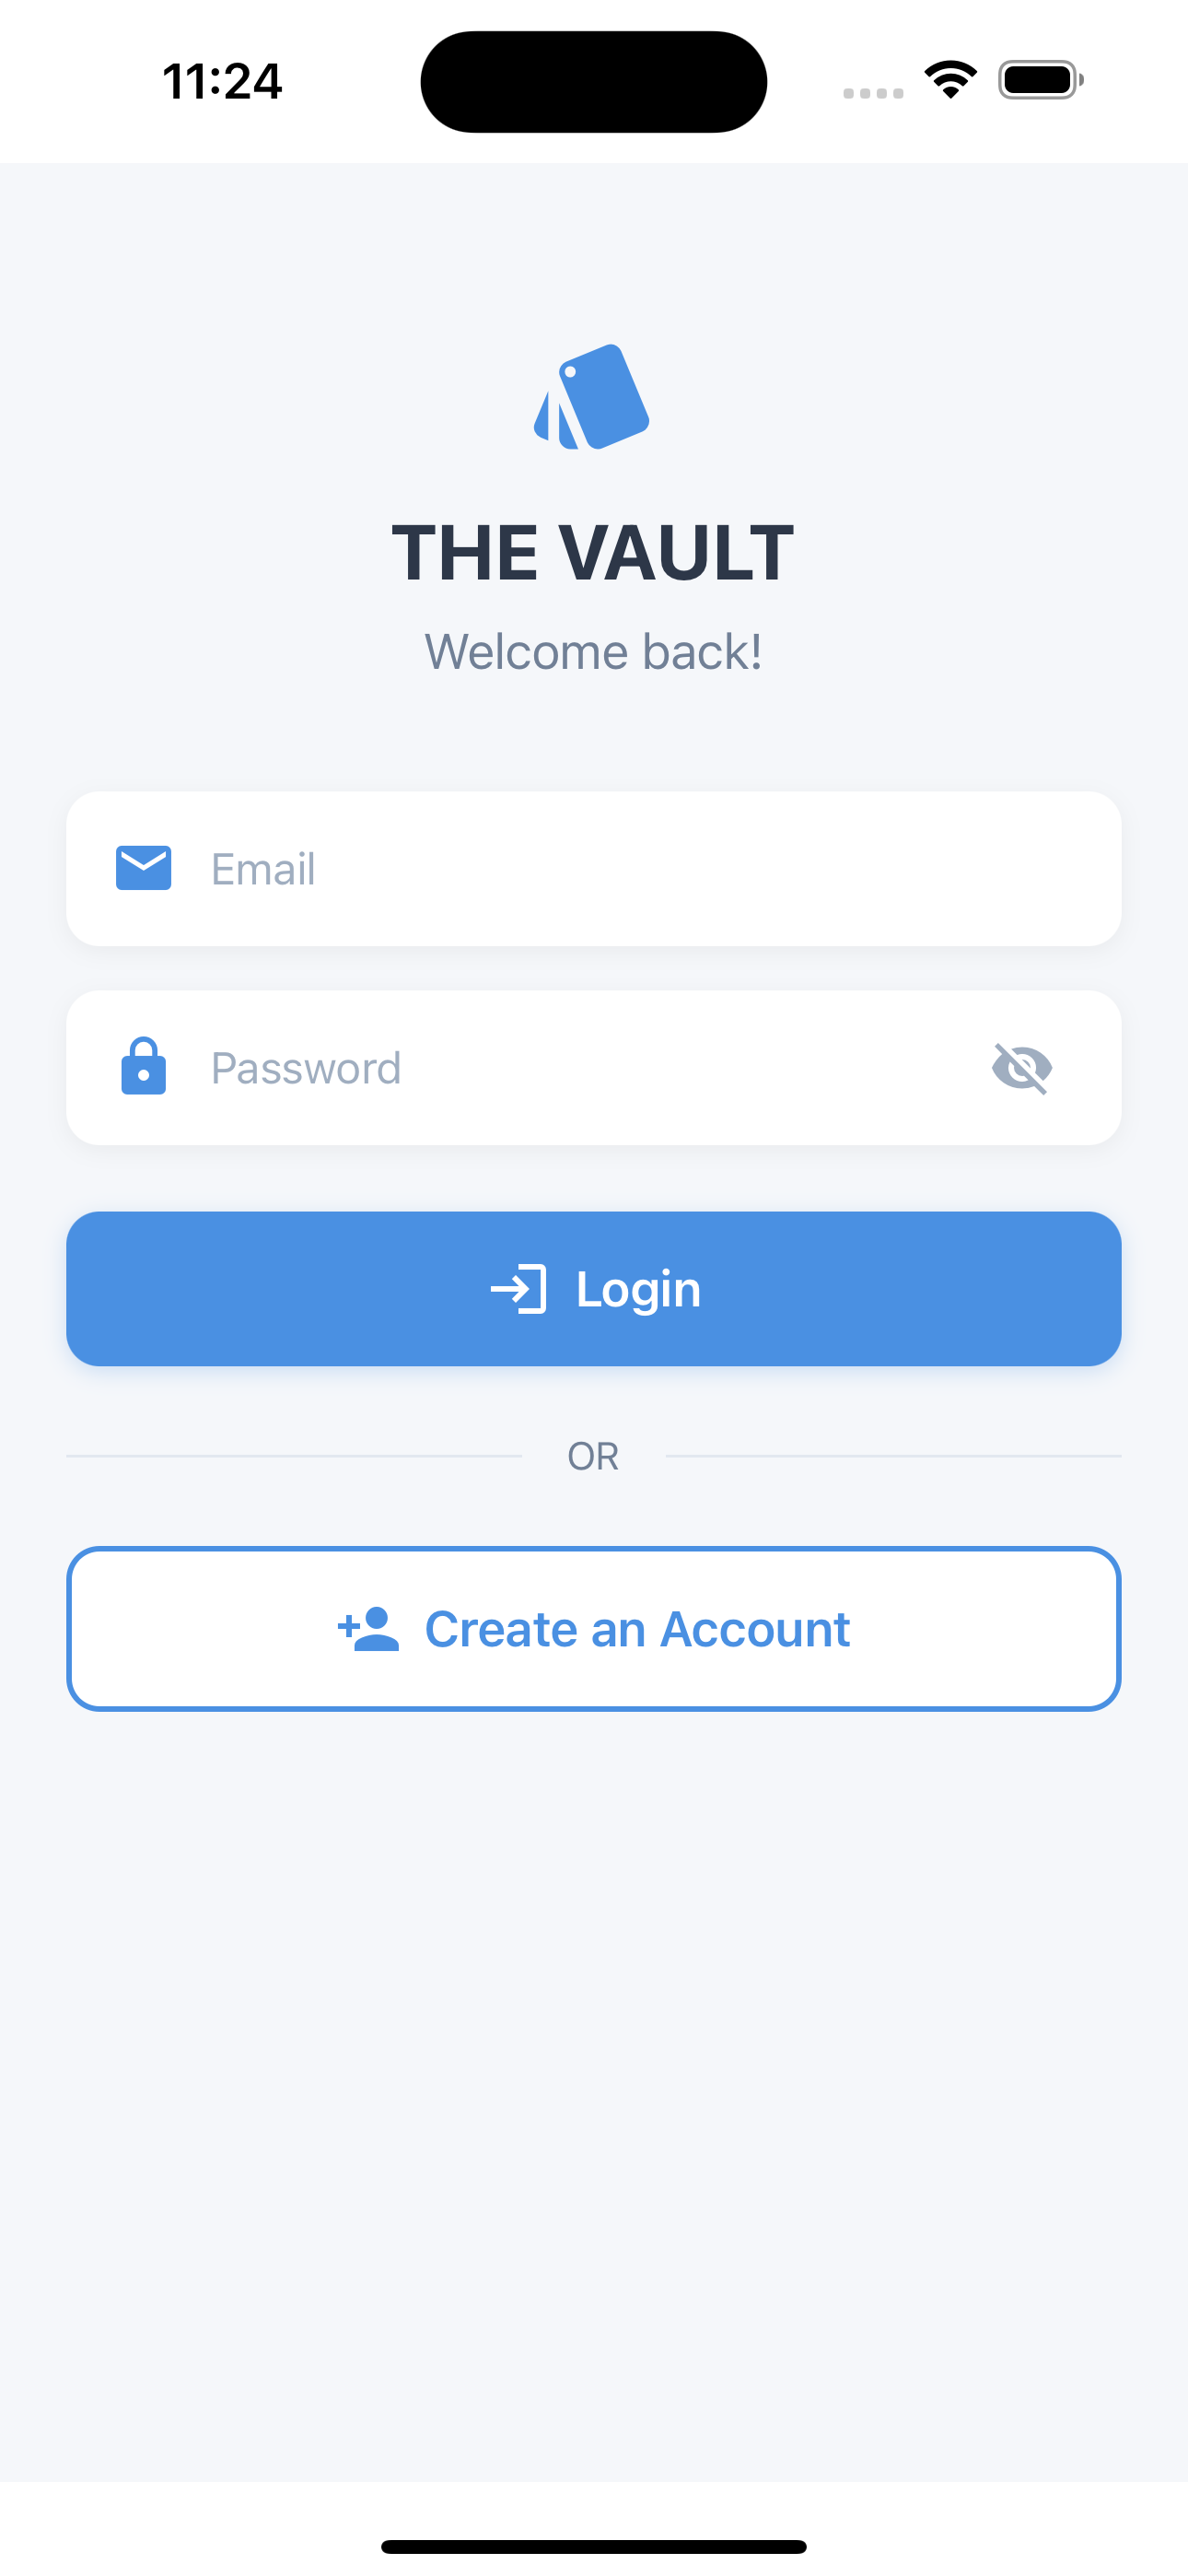
\includegraphics[width=0.3\textwidth]{exampleis-master/figures/loginscreen.png}}
    \qquad % Adds horizontal spacing between the images
    % Second Subfloat: Signup Screen
    \subfloat[Signup screen - new user registration.\label{fig:signup}]
    {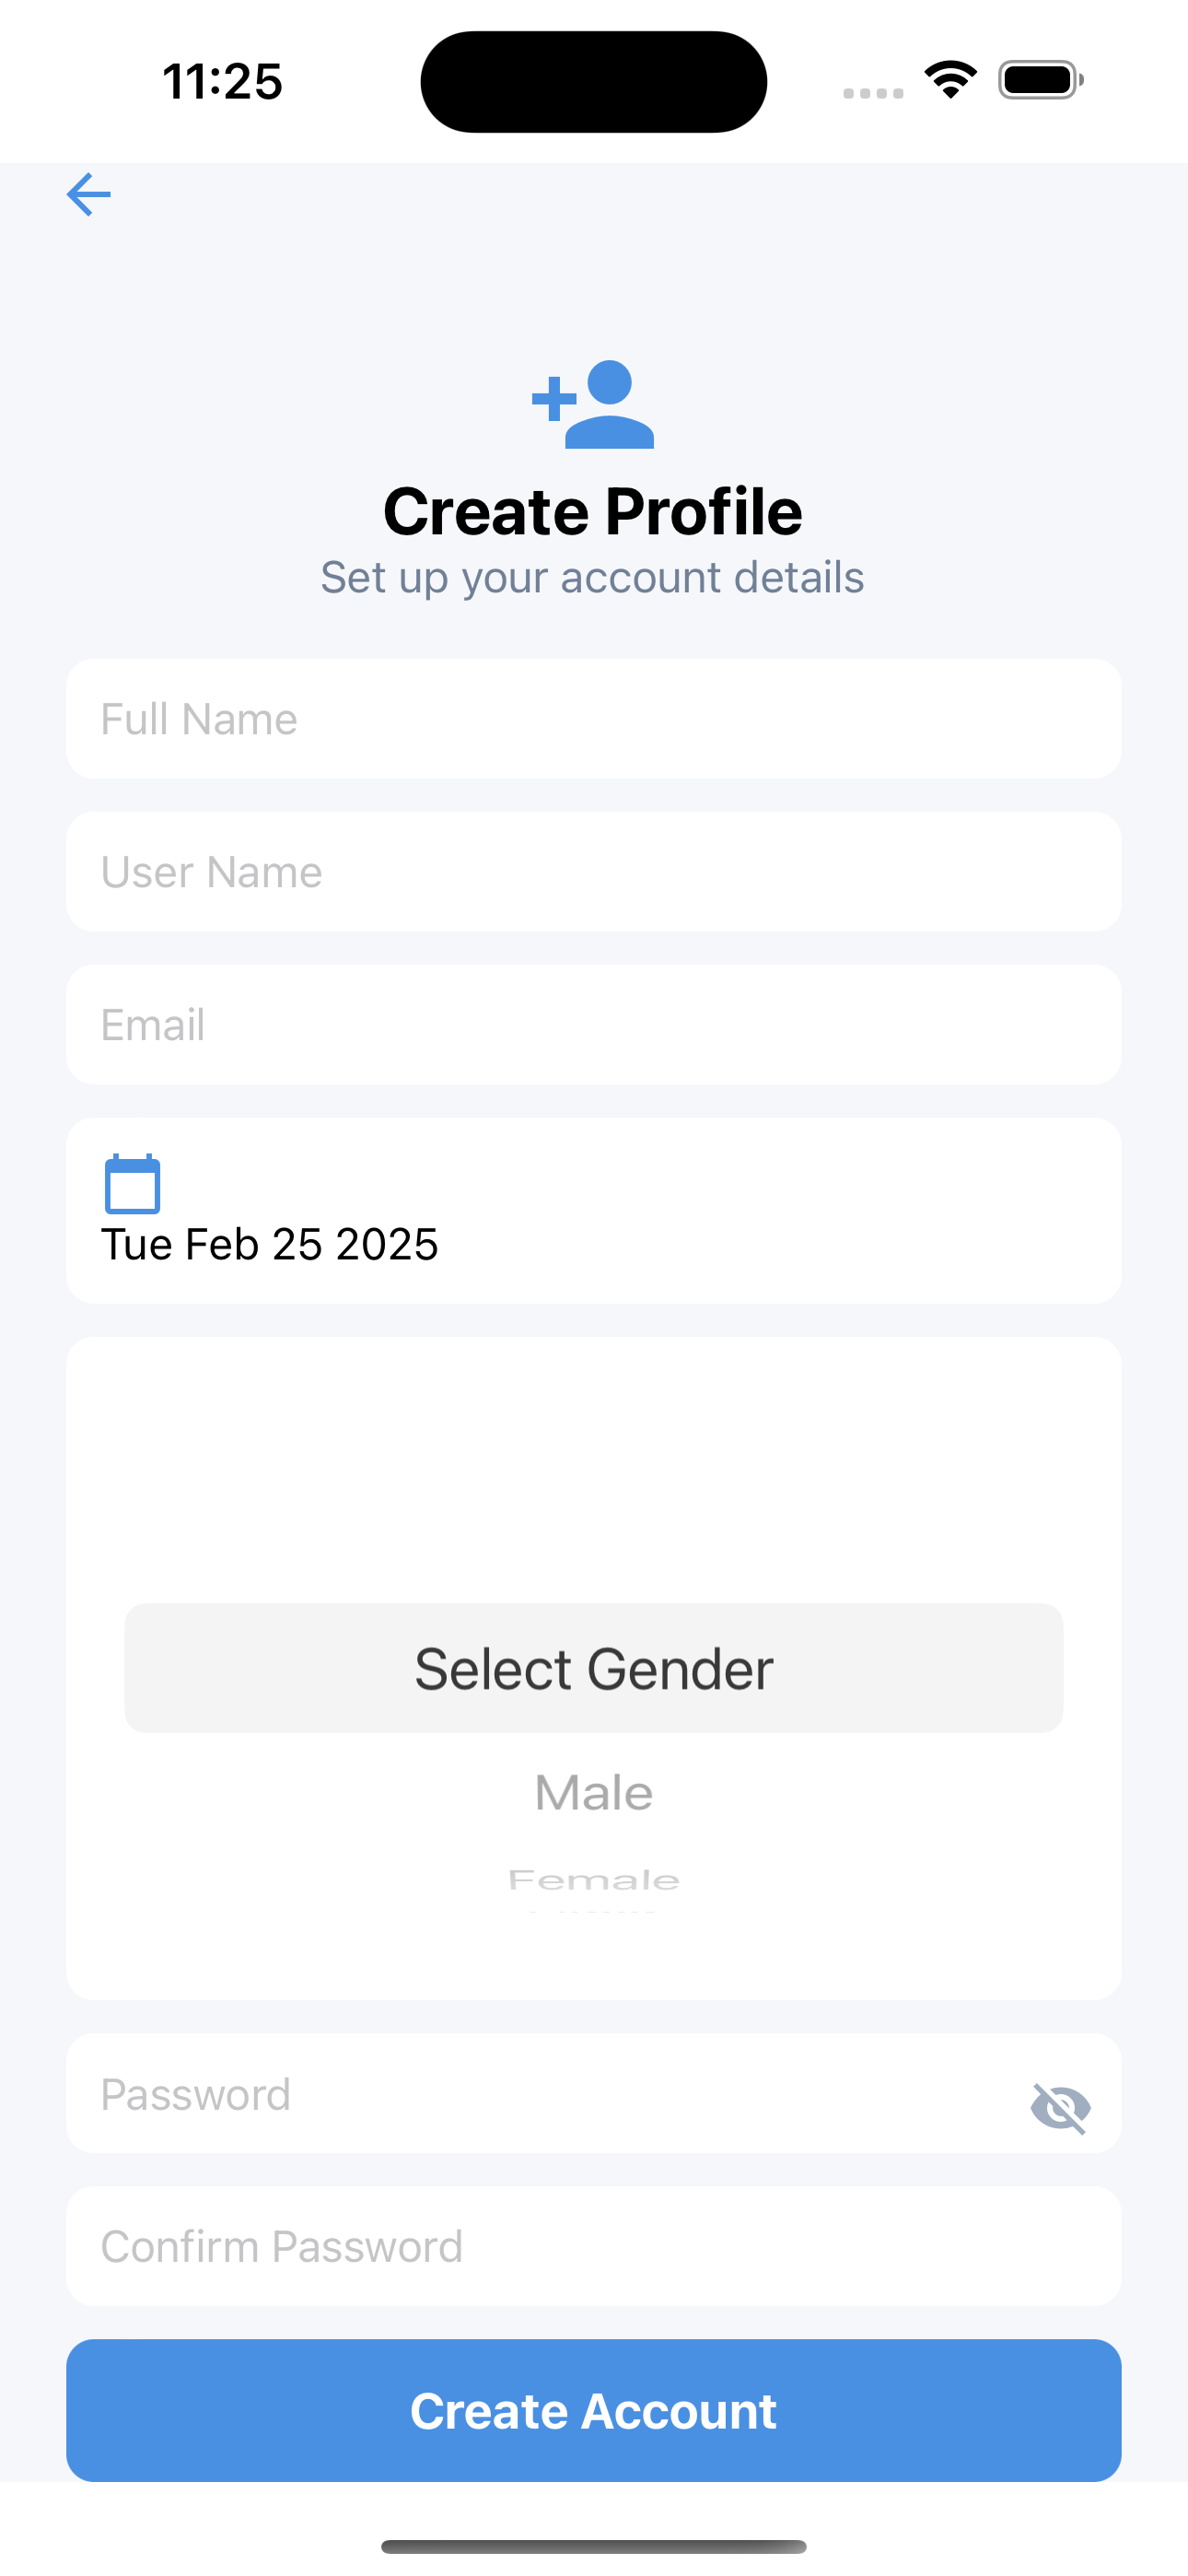
\includegraphics[width=0.3\textwidth]{exampleis-master/figures/signupscreen.png}}
    \caption{Authentication flow: users can sign up for a new account or log in to access their personalized wardrobe.}
    \label{fig:auth_flow}
\end{figure}

This redirection ensures that authenticated users can immediately access their personalized wardrobe without manual navigation. Conversely, if the user is not authenticated \textbf{(Line 17)}, they are redirected to the Login Screen \textbf{(Line 18)} to sign in as shown in Figure \ref{fig:login}. The use of \texttt{router.replace()}also prevents users from navigating back to the login screen after successfully logging in, maintaining a logical and secure flow throughout the app.

\begin{figure}[h]
    \centering
    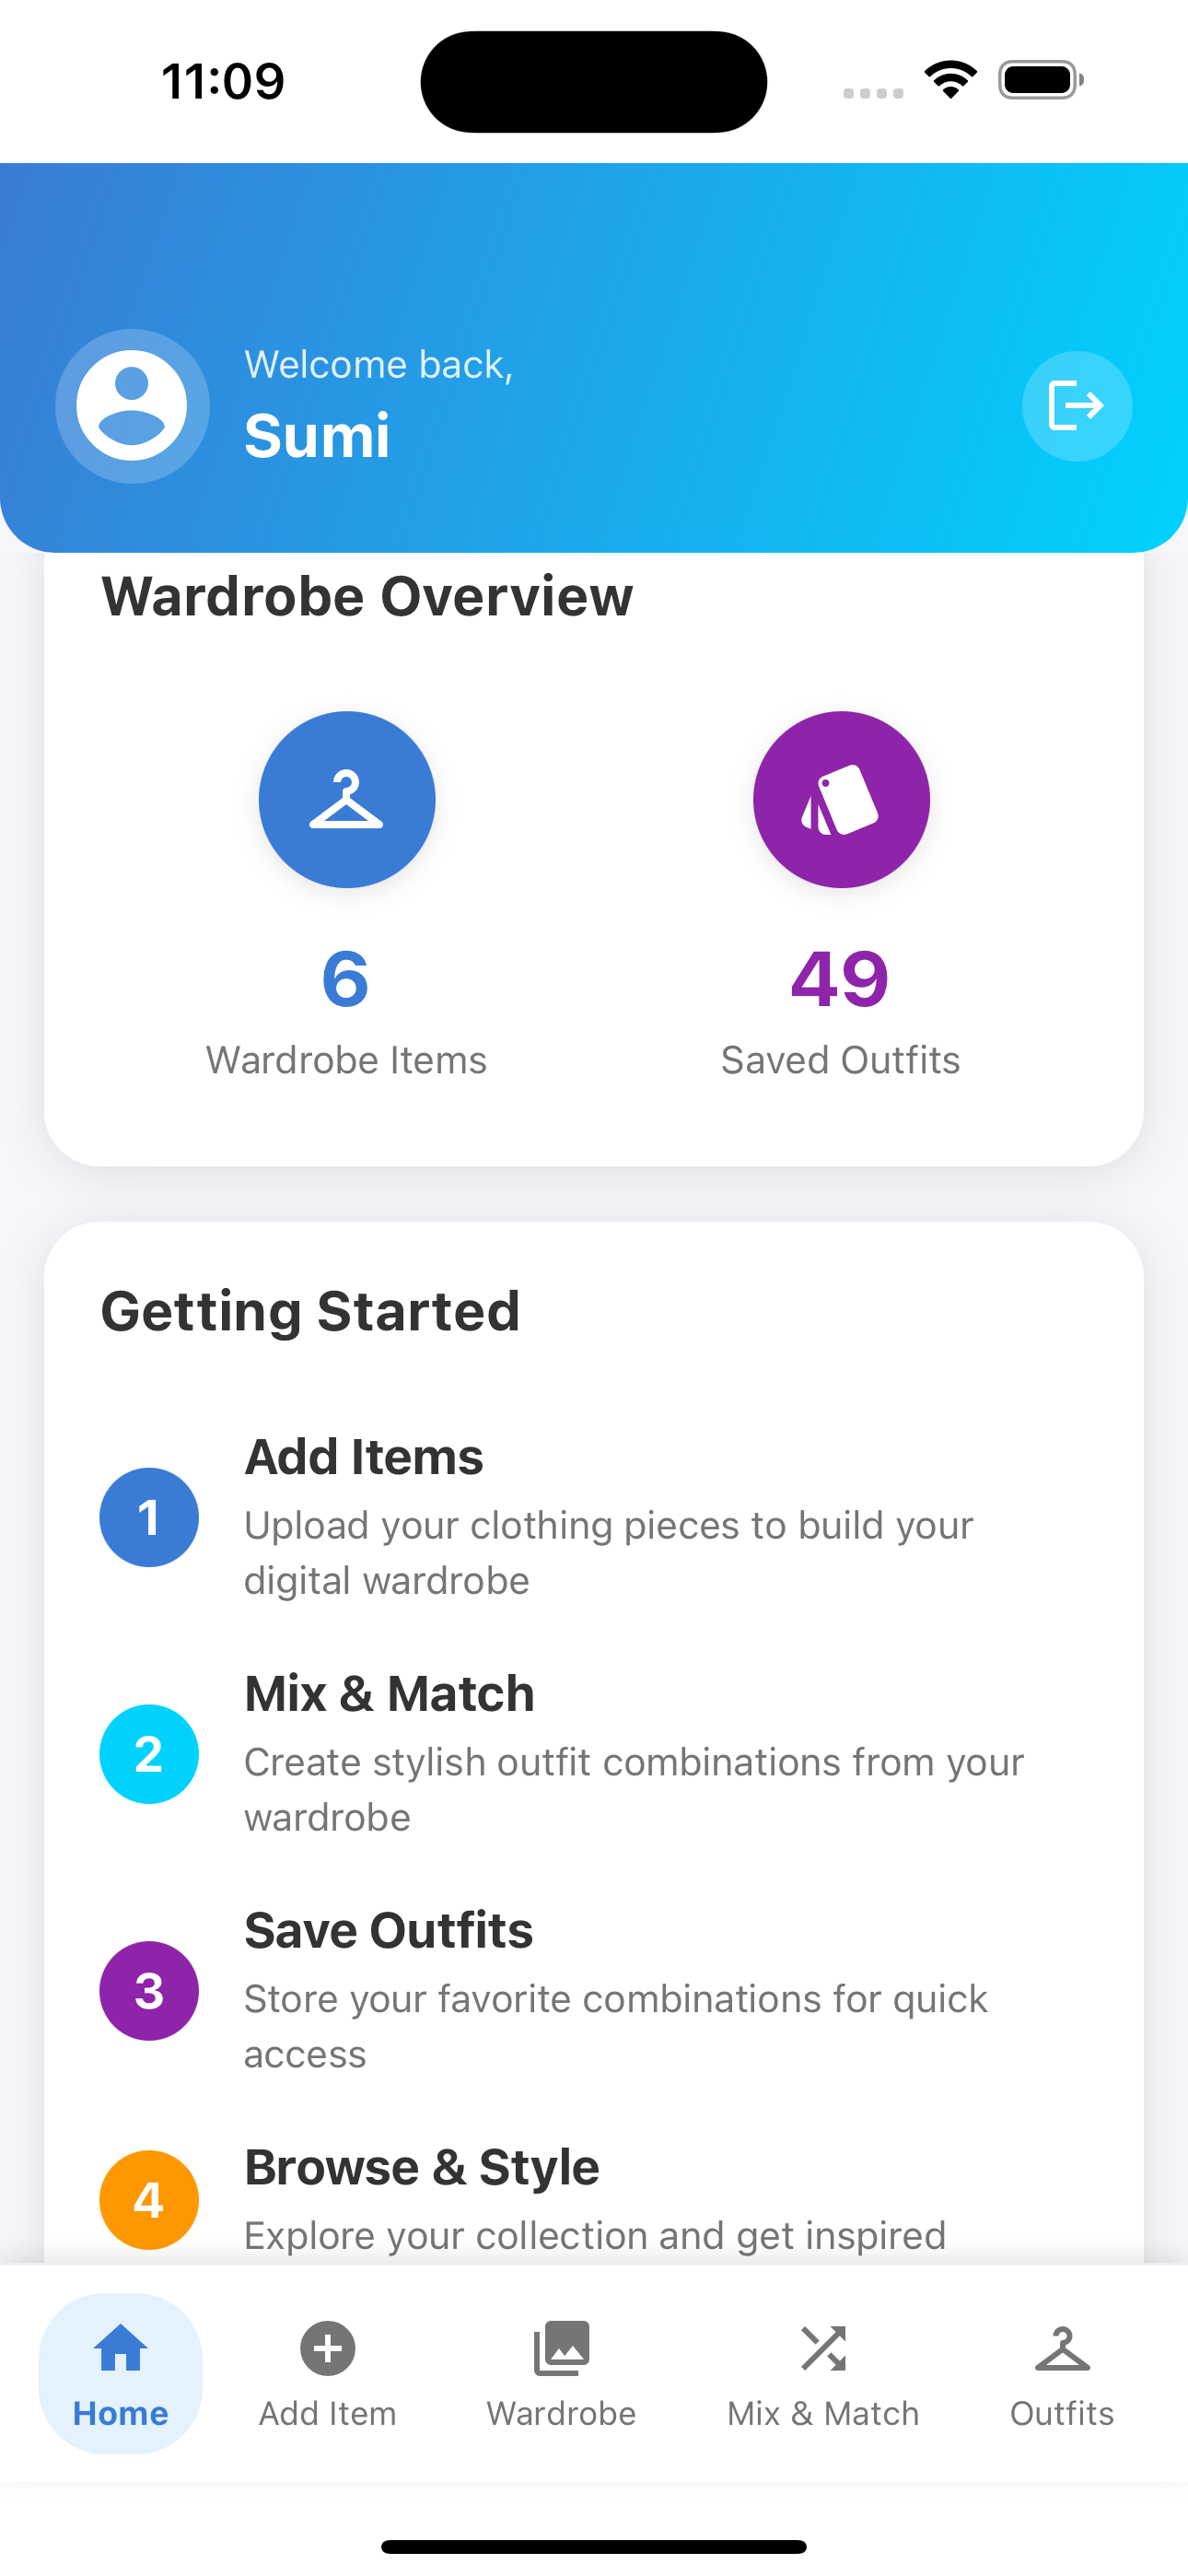
\includegraphics[width=0.3\textwidth]{exampleis-master/figures/homescreen.png}
    \caption{Home screen - user dashboard after successful login}
    \label{fig:home}
\end{figure}


The \texttt{unsubscribe} function \textbf{(Line 20)} returned from \texttt{onAuthStateChanged} ensures that Firebase stops listening for authentication changes when the component is no longer active, improving performance and preventing memory leaks.

Finally, if the authentication check is complete \textbf{(Line 23)} (\texttt{loading} is \texttt{false}), the component returns \texttt{null} \textbf{(Line 27)}, as the routing logic has already directed the user to the appropriate screen. This implementation ensures that the user experience remains smooth, secure, and responsive, with real-time authentication checks providing instant feedback and navigation adjustments based on user actions.


\subsection{Data Management and Storage}
Once a user is authenticated and navigates through the app, My Digital Wardrobe relies on Firebase Cloud Storage and Firestore to handle image uploads and organize wardrobe data. These services work together to ensure that clothing images are securely stored while metadata—such as category, upload date, and user information—remains easily accessible for browsing and outfit creation.

When a user uploads a clothing item, the image file is stored in Firebase Cloud Storage, while Firestore maintains details about the item. This separation ensures that large image files do not slow down database operations, while structured metadata enables quick filtering and retrieval.

The process begins when a user selects an image to upload. The image file is converted into a format suitable for storage, assigned a unique name to prevent overwrites, and uploaded to Firebase Storage. Once the upload is complete, a publicly accessible URL is generated and stored in Firestore along with relevant metadata, as shown in Listing \ref{lst:Firebaseupload}
\begin{lstlisting}[caption={Storing images and metadata in \texttt{Firebaseupload.js}},label=lst:Firebaseupload]
import { ref, uploadBytes, getDownloadURL } from "firebase/storage";
import { collection, addDoc } from "firebase/firestore";
import { storage, db } from "./firebase";

export const uploadImageToFirebase = async (imageUri, category) => {
    const imageName = `${Date.now()}-${imageUri.split("/").pop()}`;
    const storageRef = ref(storage, `wardrobe/${category}/${imageName}`);
    const response = await fetch(imageUri);
    const blob = await response.blob();

    await uploadBytes(storageRef, blob);
    const downloadUrl = await getDownloadURL(storageRef);
    await addDoc(collection(db, "wardrobeItems"), {
        imageUrl: downloadUrl,
        category,
        uploadedAt: new Date(),
    });
};
\end{lstlisting}

This function ensures that every image is stored efficiently while keeping metadata structured for easy retrieval. With Firestore tracking categories such as "Tops" and "Bottoms," wardrobe items are automatically sorted and can be displayed within their respective sections.

Once an item is stored, it becomes accessible through the app’s browsing features. When users navigate to \textbf{WardobeScreen} \ref{fig:wardrobe_screen} , a query to Firestore retrieves the relevant clothing items, grouping them by category. This ensures an easy browsing experience, allowing users to scroll through their wardrobe without delays.

The integration of Firebase services provides a foundation for efficient wardrobe management. Users can upload clothing, categorize items, and retrieve them when needed. This structured approach ensures that wardrobe data remains organized and accessible at all times.


\subsection{Image Uploading and Categorization}

Following user authentication and storing their data, the Upload Screen plays a vital role in My Digital Wardrobe by enabling users to add clothing items from their device’s gallery. Once authenticated and directed to the \textbf{Home Screen} as seen in Figure \ref{fig:home}, users can navigate to the \textbf{Upload Screen} \ref{fig:image_upload_flow}, where they can select and upload images representing their wardrobe items. This functionality is essential for personalizing the wardrobe experience and serves as the starting point for organizing and creating outfits within the app.

The \textbf{Upload Screen} in Figure \ref{fig:gallery_access} provides an intuitive interface where users can select multiple images at once, categorize them into tops and bottoms, and upload them securely. The integration between Expo’s  \texttt{ImagePicker} API and ensures that this process is efficient. Additionally, relevant metadata, mentioned in Chapter \ref{chap:Chapter4} such as category and upload timestamp, is stored in Firestore, allowing for easy organization and retrieval of wardrobe items later.

The core logic for the image uploading feature resides in the \texttt{upload.js} file. The following code snippet in Listing \ref{lst:picker} outlines how \texttt{ImagePicker} and Firebase services collaborate to process and store images:
\begin{lstlisting}[caption={Image picker integration in \texttt{ upload.js}},label=lst:picker]
import * as ImagePicker from "expo-image-picker";
import { uploadImageToFirebase } from "./firebaseUpload";

const pickImages = async (category) => {
    const result = await ImagePicker.launchImageLibraryAsync({ allowsMultipleSelection: true });
    if (!result.canceled) {
        result.assets.forEach(async (asset) => {
            await uploadImageToFirebase(asset.uri, category);
        });
    }
};
\end{lstlisting}

The image uploading process in \textbf{My Digital Wardrobe} begins by importing essential dependencies \textbf{(Lines 1–2)}. The \texttt{ImagePicker} module from Expo allows users to select images from their device’s gallery, forming the core of the Upload Screen's image selection interface. The \texttt{uploadImageToFirebase} function is a custom utility responsible for uploading selected images to Firebase Storage and saving relevant metadata in Firestore. The \texttt{pickImages} function is then defined \textbf{(Line 3)} as an asynchronous function (\texttt{async}), allowing the app to handle time-consuming tasks like image uploads without freezing the user interface. This function accepts a \texttt{category} parameter, ensuring that each uploaded image is linked to a specific user-selected category, supporting the Upload Screen's category selection interface.

The next step involves launching the image picker \textbf{(Line 4)}. The \texttt{launchImageLibraryAsync} function opens the device’s gallery, allowing users to select multiple images at once, thanks to the \texttt{allowsMultipleSelection:true} setting. Figure \ref{fig:gallery_access}  shows this multi-select capability that enhances convenience when users add several wardrobe items simultaneously, contributing to the Upload Screen's multi-select gallery view. Once images are selected, the function checks the selection \textbf{(Line 5)} using the \texttt{if (!result.canceled)} condition to confirm that the user did not cancel the process, reflecting the Upload Screen's cancel/upload confirmation state. If images are present, the app loops through each image \textbf{(Line 6)} using \texttt{result.assets.forEach} for further processing.

The uploading phase follows \textbf{(Line 7)}, where the \texttt{uploadImageToFirebase} function is invoked for each selected image. This function receives the URI (the file location on the user’s device) and its category as parameters. The \texttt{await} keyword ensures that each image is completely uploaded before the next begins, preventing incomplete uploads and supporting the Upload Screen's upload progress feedback. Finally, after all selected images have been processed \textbf{(Line 9)}, the function completes. By this point, all images are securely stored in Firebase Storage, with metadata saved in Firestore for easy retrieval shown in Figure \ref{fig:firestore_collections}. These items are now ready for display in the Gallery Screen, categorized and organized for users to browse, mix, and match when creating outfits.

\begin{figure}[!ht]
    \centering
    % First Subfloat: Upload Screen
    \subfloat[Upload screen - users can upload images from their device.\label{fig:upload_screen}]
    {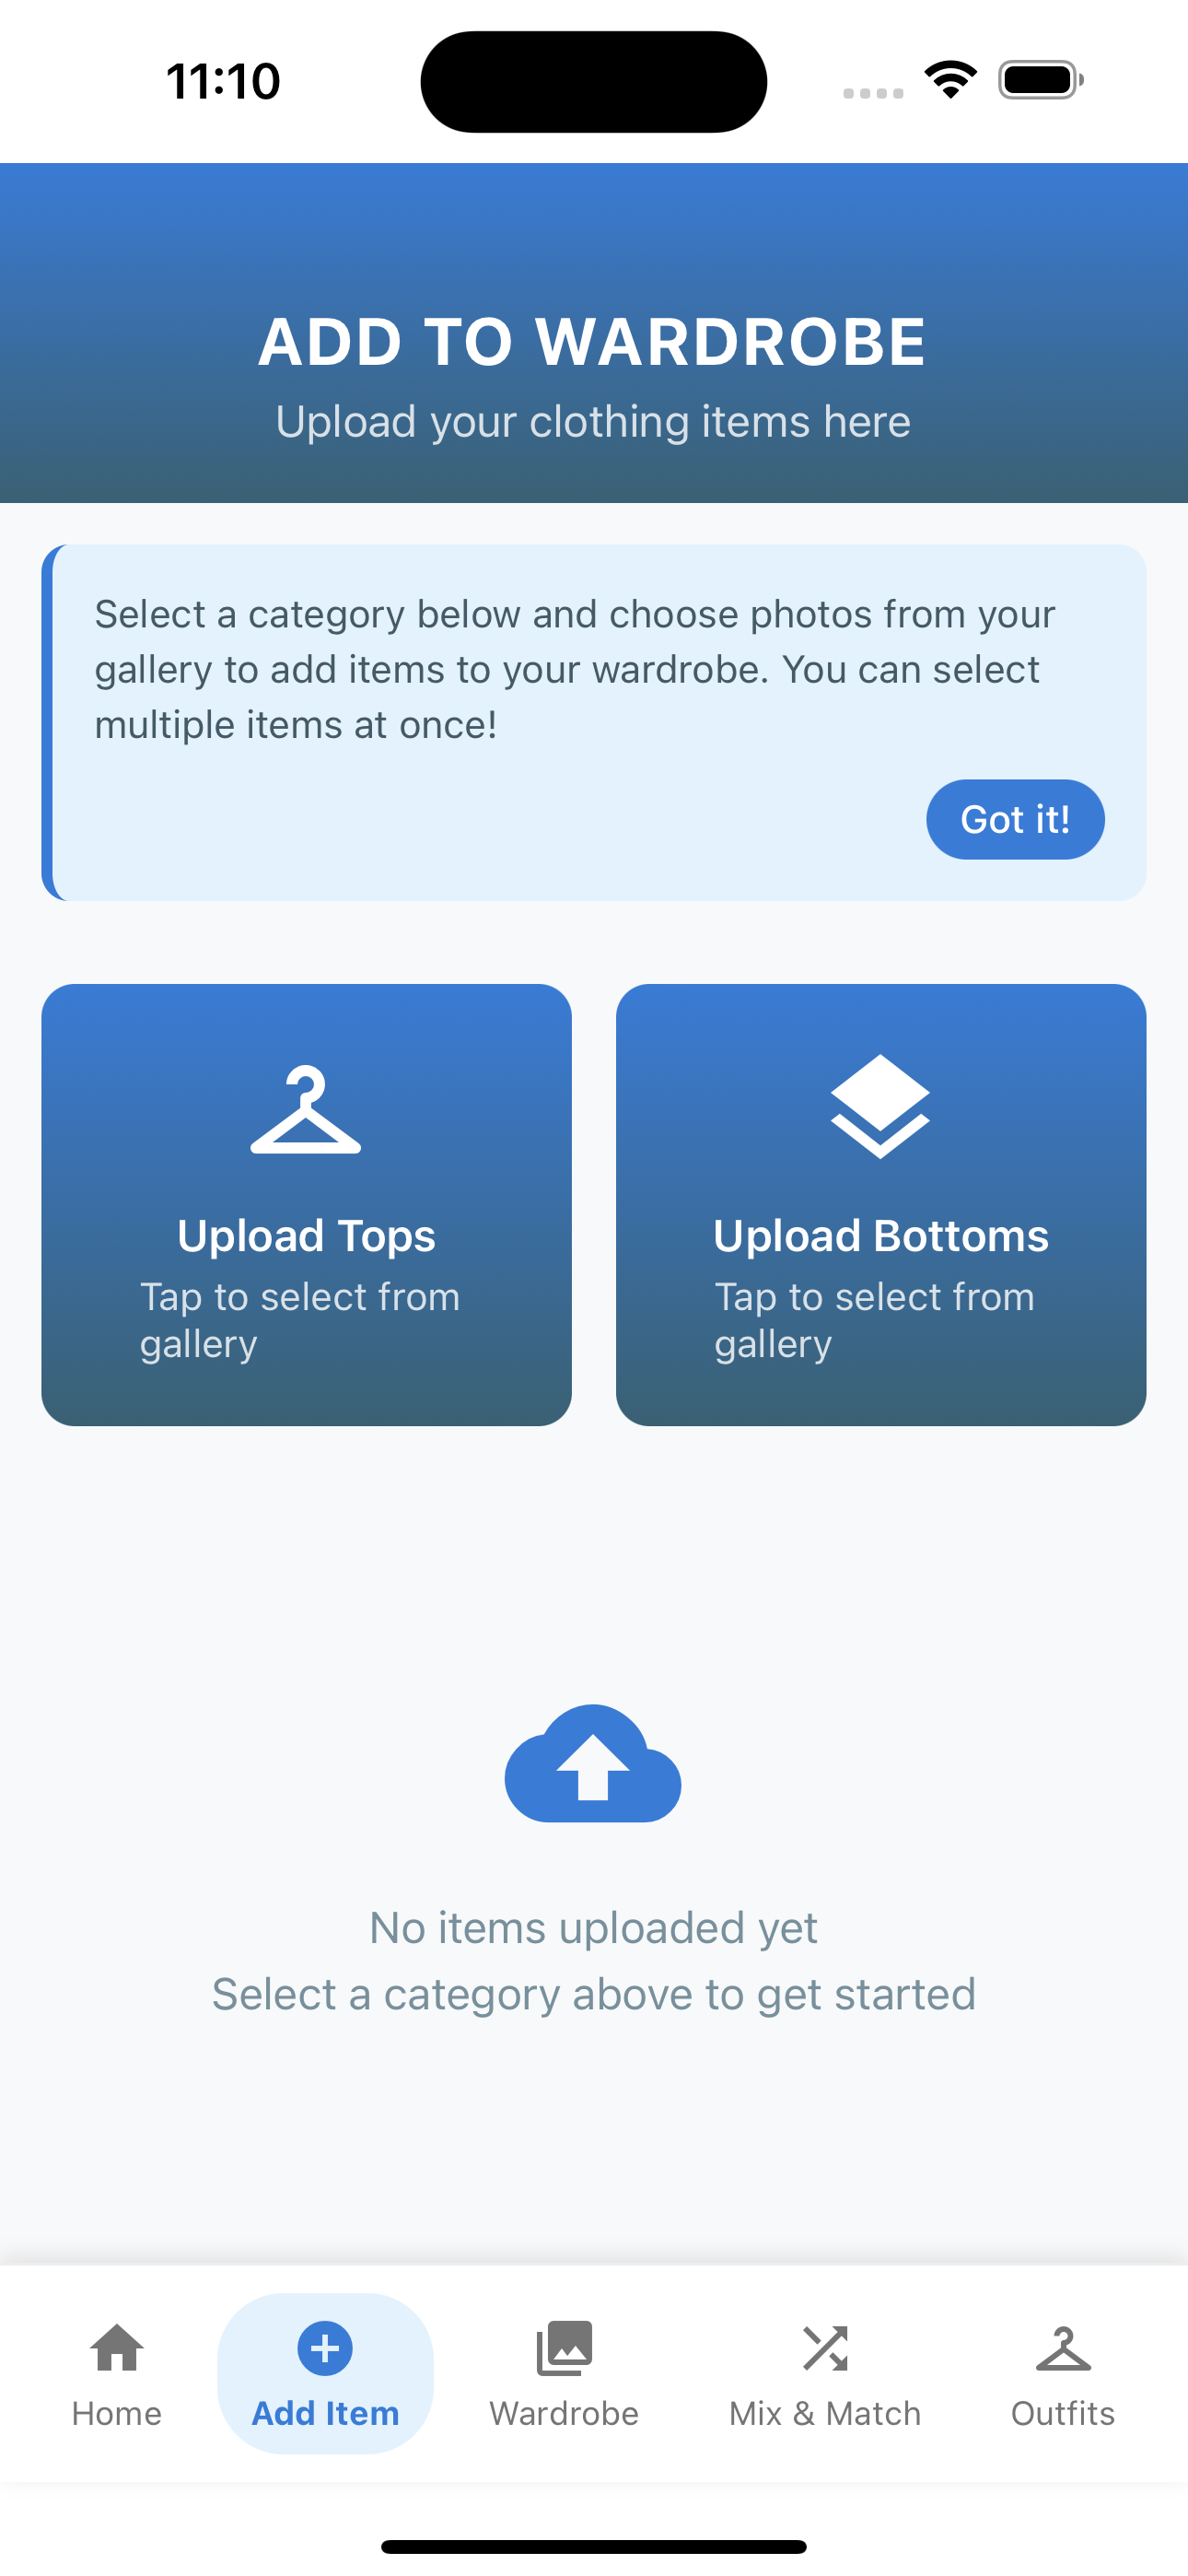
\includegraphics[width=0.3\textwidth]{exampleis-master/figures/uploadscreen.png}}
    \qquad % Adds horizontal spacing between the images
    % Second Subfloat: User Gallery Access Screen
    \subfloat[Gallery access screen - users can select images directly from their device's gallery.\label{fig:gallery_access}]
    {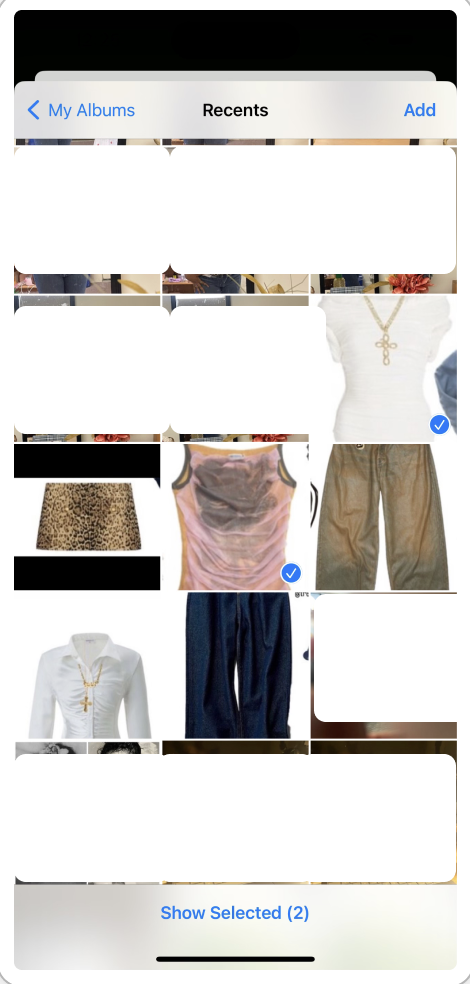
\includegraphics[width=0.3\textwidth]{exampleis-master/figures/defice.png}}
    \caption{Image upload process: users can either upload images directly or access their device's gallery for selection.}
    \label{fig:image_upload_flow}
\end{figure}

Effective wardrobe management in \textit{}{My Digital Wardrobe} is made possible through \textbf{ categorization} and \textbf{interactive browsing}. Users can upload clothing items, assign them to predefined categories, and browse their wardrobe efficiently. These features allow for quick outfit selection, enabling users to mix and match clothing pieces. This section explains how these functionalities are implemented, highlighting their interaction with Firebase and Expo's navigation features.

Each clothing item uploaded to the app is categorized as either a "Top" or a "Bottom" and stored in Firebase Firestore along with its metadata. Categorization simplifies retrieval and filtering, ensuring that users can efficiently browse their wardrobe. The function \texttt{fetchImages}, shown in Listing \ref{lst:fetch_images}, retrieves wardrobe items from Firestore and dynamically assigns them a category.

\begin{lstlisting}[caption={Fetch images by category in \texttt{GalleryScreen.js}}, label={lst:fetch_images}]
const fetchImages = async () => {
    const querySnapshot = await getDocs(collection(db, "wardrobeItems"));
    const itemData = querySnapshot.docs.map((doc) => ({
        ...doc.data(),
        id: doc.id,
        url: doc.data().imageUrl,
        category: doc.data().category?.toLowerCase().includes("top")
            ? "Tops"
            : "Bottoms",
    }));
    setImages(itemData);
};
\end{lstlisting}

This function queries Firestore for all wardrobe items, extracts metadata including the image URL and category, converts category names to lowercase to ensure consistency, and assigns each item to either "Tops" or "Bottoms". The retrieved images are then grouped by category to provide a structured browsing experience, as seen in Listing \ref{lst:group_images}:

\begin{lstlisting}[caption={Group images by category}, label={lst:group_images}]
const groupedImages = images.reduce((acc, item) => {
    if (!acc[item.category]) {
        acc[item.category] = [];
    }
    acc[item.category].push(item);
    return acc;
}, {});
\end{lstlisting}

To enhance user interaction, My Digital Wardrobe incorporates interactive navigation, allowing users to scroll through wardrobe items. Expo's built-in navigation capabilities enable tap selection and horizontal scrolling. The \texttt{handleImageSelect} function, found in Listing \ref{lst:image_select}, enables users to select wardrobe items by tapping.

\begin{lstlisting}[caption={Image selection handler}, label={lst:image_select}]
const handleImageSelect = (item) => {
    if (item.category === "Tops") {
        setSelectedTop(selectedTop?.id === item.id ? null : item);
    } else if (item.category === "Bottoms") {
        setSelectedBottom(selectedBottom?.id === item.id ? null : item);
    }
};
\end{lstlisting}

This implementation allows users to tap an item to select it, tap again to deselect it, and independently choose tops and bottoms before creating an outfit. A visual cue is provided to indicate selected items as demonstarted in Figure \ref{fig:selection_ visual_aid}. Conditional styling in Listing \ref{lst:selected_style} highlights selections with a colored border.

\begin{lstlisting}[caption={Conditional styling for selected items}, label={lst:selected_style}]
const styles = StyleSheet.create({
    selectedImage: {
        borderWidth: 3,
        borderColor: "#FF1493",
    },
});
\end{lstlisting}

\begin{figure}[!ht]
    \centering
    % First Subfloat: Warbrobe Screen
    \subfloat[Wardrobe screen - displays categorized wardrobe items.\label{fig:wardrobe_screen}]
    {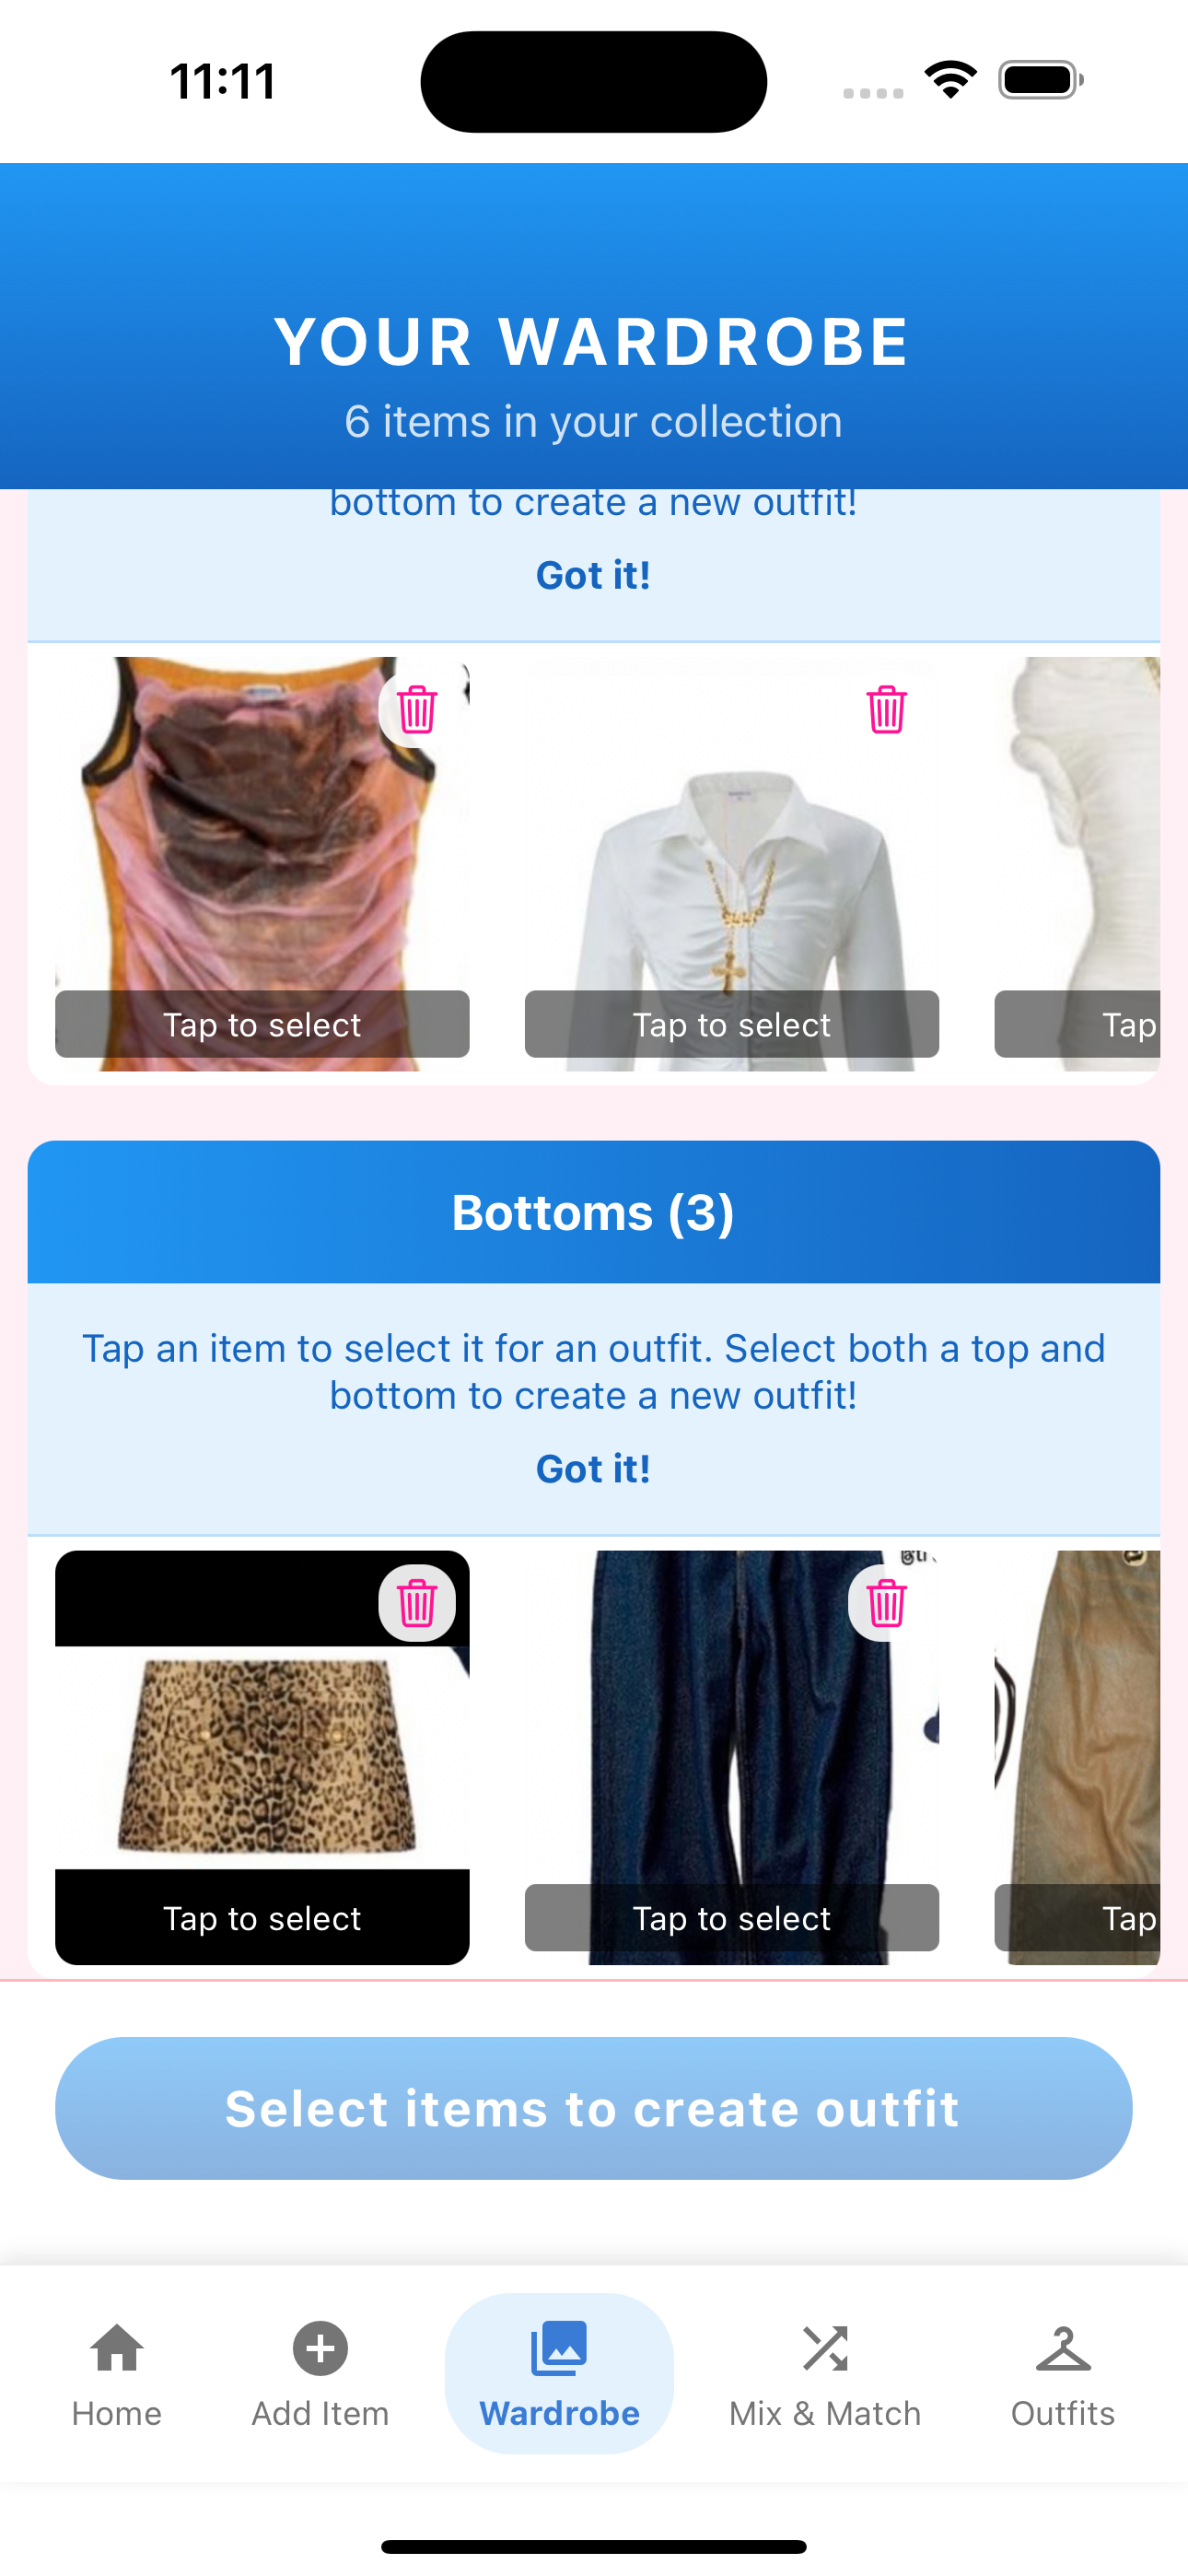
\includegraphics[width=0.3\textwidth]{exampleis-master/figures/wardrobe1.png}}
    \qquad % Adds horizontal spacing between the images
    % Second Subfloat: Outfit Screen
    \subfloat[Warbrobe screen - users can see thier selection.\label{fig:cameraroll_screen}]
    {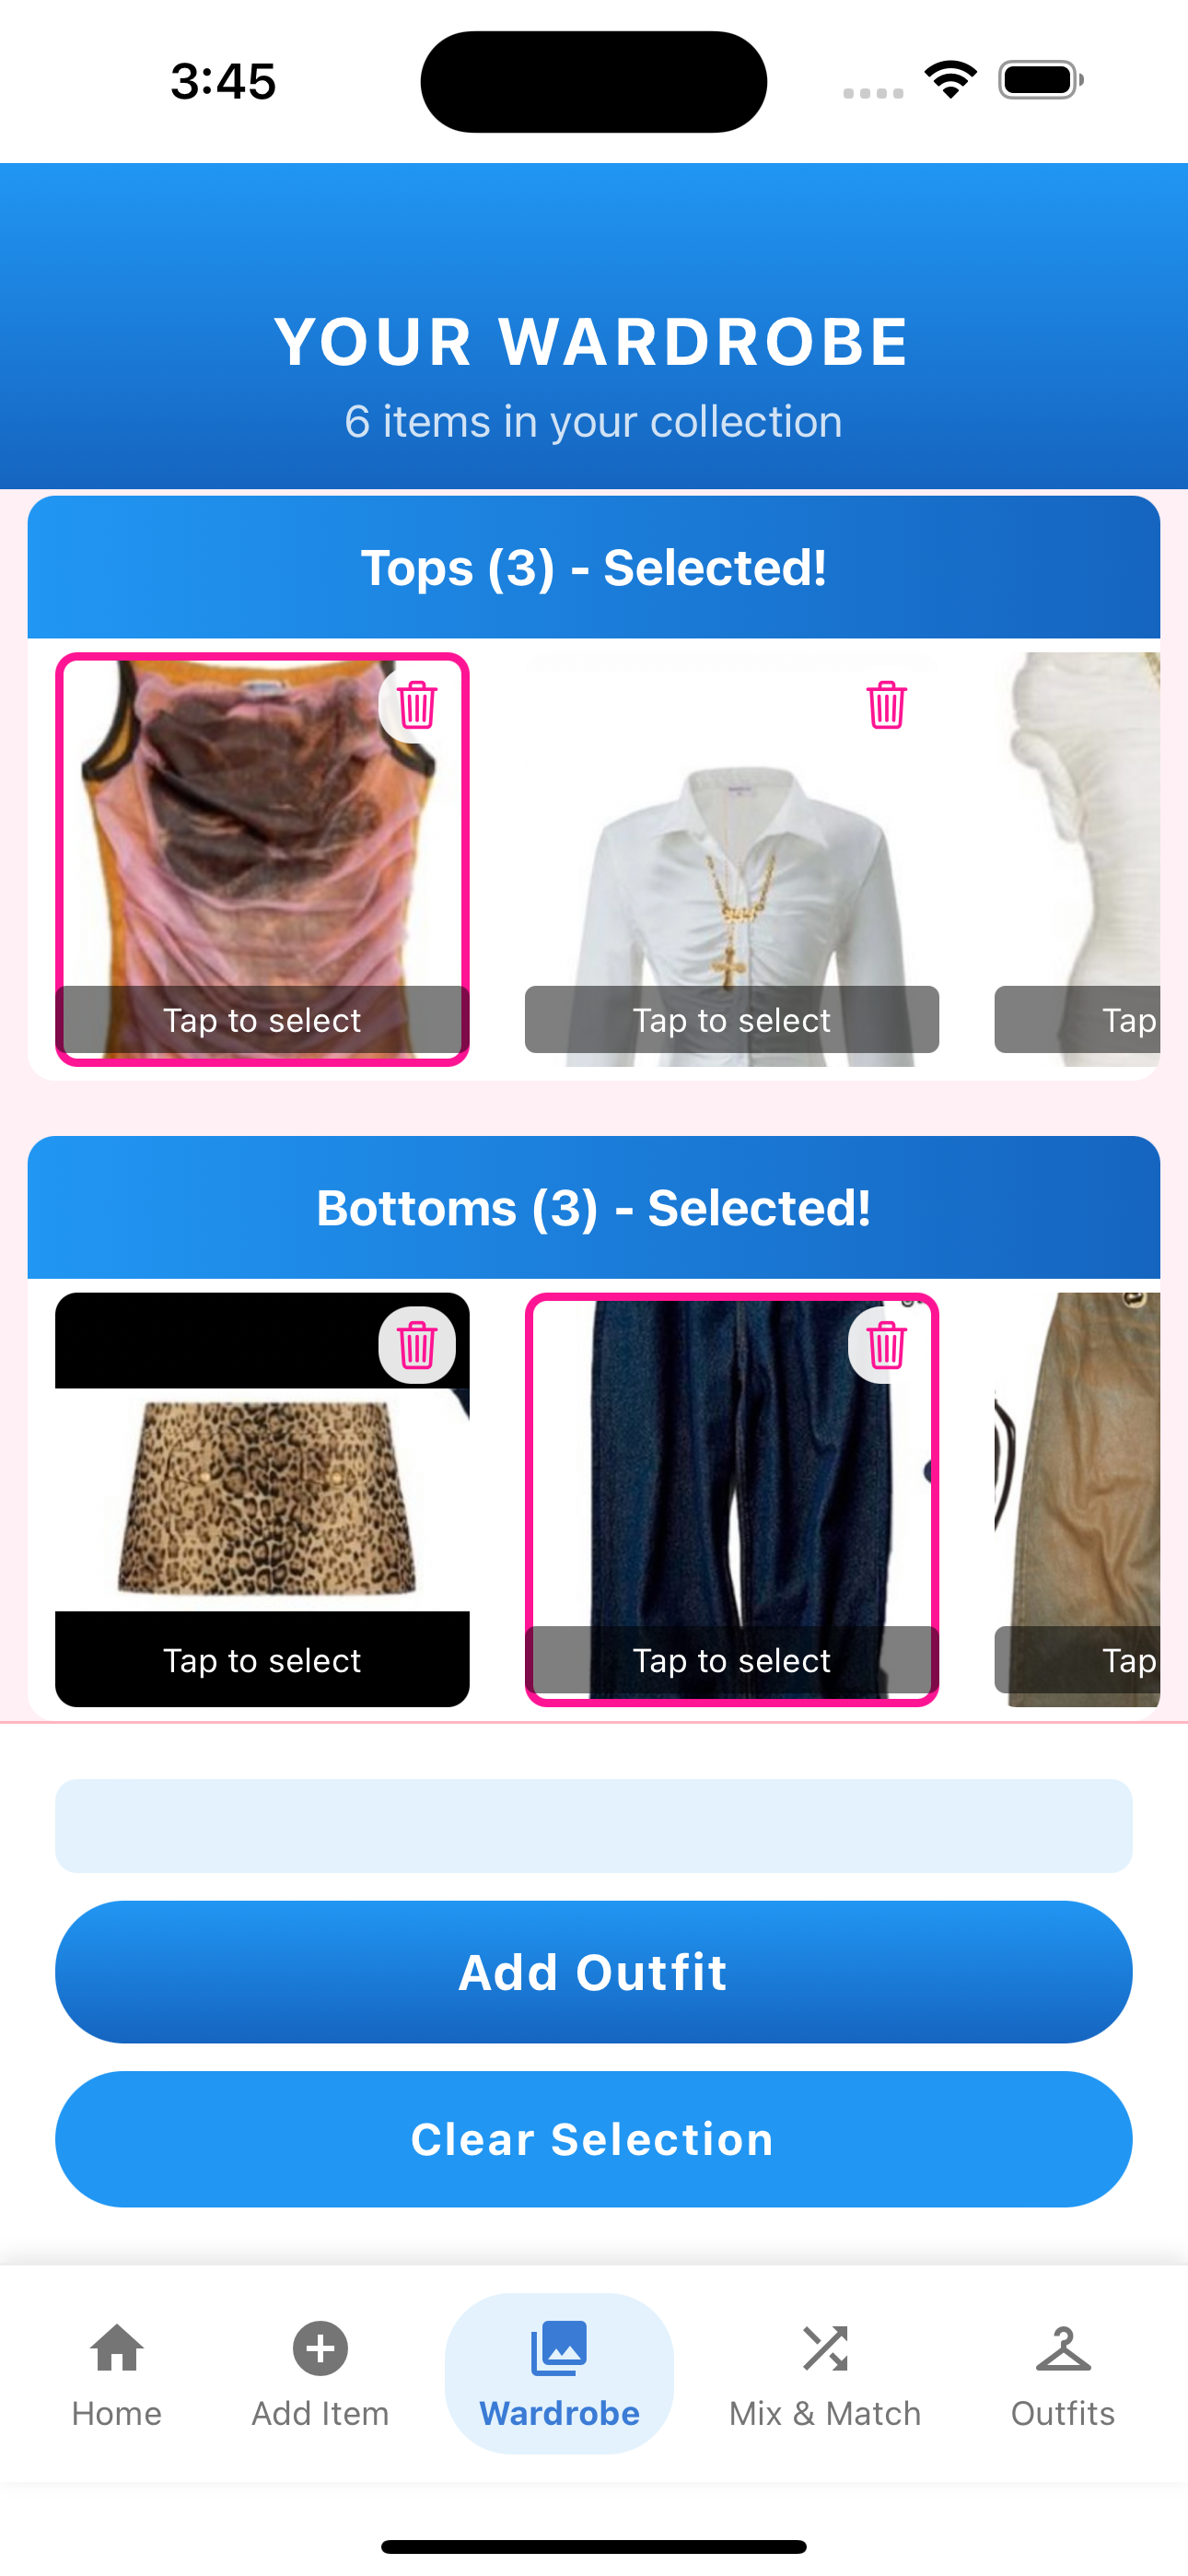
\includegraphics[width=0.3\textwidth]{exampleis-master/figures/wardrobe3.png}}
    \caption{Wardrobe browsing and outfit management: users can browse their categorized wardrobe in the wardrobe screen and add their selection}
    \label{fig:selection_ visual_aid}
\end{figure}

Once users have selected a top and bottom, they can preview the combination in OutfitScreen as shown in Figure \ref{fig:cameraroll_screen}. The function \texttt{renderOutfitCard} in Listing \ref{lst:outfit_card} dynamically displays selected outfit items.

\begin{lstlisting}[caption={Render outfit card in \texttt{OutfitScreen.js}}, label={lst:outfit_card}]
const renderOutfitCard = ({ item }) => (
    <View style={styles.outfitCard}>
        <Image source={{ uri: item.top }} style={styles.outfitImage} />
        <Image source={{ uri: item.bottom }} style={styles.outfitImage} />
        <Text>{item.name || "Untitled Outfit"}</Text>
    </View>
);
\end{lstlisting}

This preview ensures that users can visually assess outfit combinations before saving them. The function handleSaveOutfit in Listing \ref{lst:save_outfit}, also found in OutfitScreen.js, stores the finalized selection in Firestore.

\begin{lstlisting}[caption={Save outfit function}, label={lst:save_outfit}]
const handleSaveOutfit = async () => {
    const selectedTop = wardrobe.tops[selectedTopIndex];
    const selectedBottom = wardrobe.bottoms[selectedBottomIndex];
    await saveOutfit({ top: selectedTop, bottom: selectedBottom });
};
\end{lstlisting}

This step ensures that saved outfits can be accessed later in the Outfit Screen, where users can delete or manage their stored combinations.

Additionally, a randomization feature has been implemented as seen in Listing \ref{lst:randomize_outfit}, allowing users to generate outfit combinations automatically. This feature selects a random top and bottom from the wardrobe:

\begin{lstlisting}[caption={Randomize outfit function}, label={lst:randomize_outfit}] 
const handleRandomize = () => {
    setSelectedTopIndex(Math.floor(Math.random() * wardrobe.tops.length));
    setSelectedBottomIndex(Math.floor(Math.random() * wardrobe.bottoms.length));
};
\end{lstlisting}

\begin{figure}[!ht]
    \centering
    % First Subfloat: Warbrobe Screen
    \subfloat[Mix and match screen - displays selected items from Wardrobe.\label{fig:mixandmatch_screen}]
    {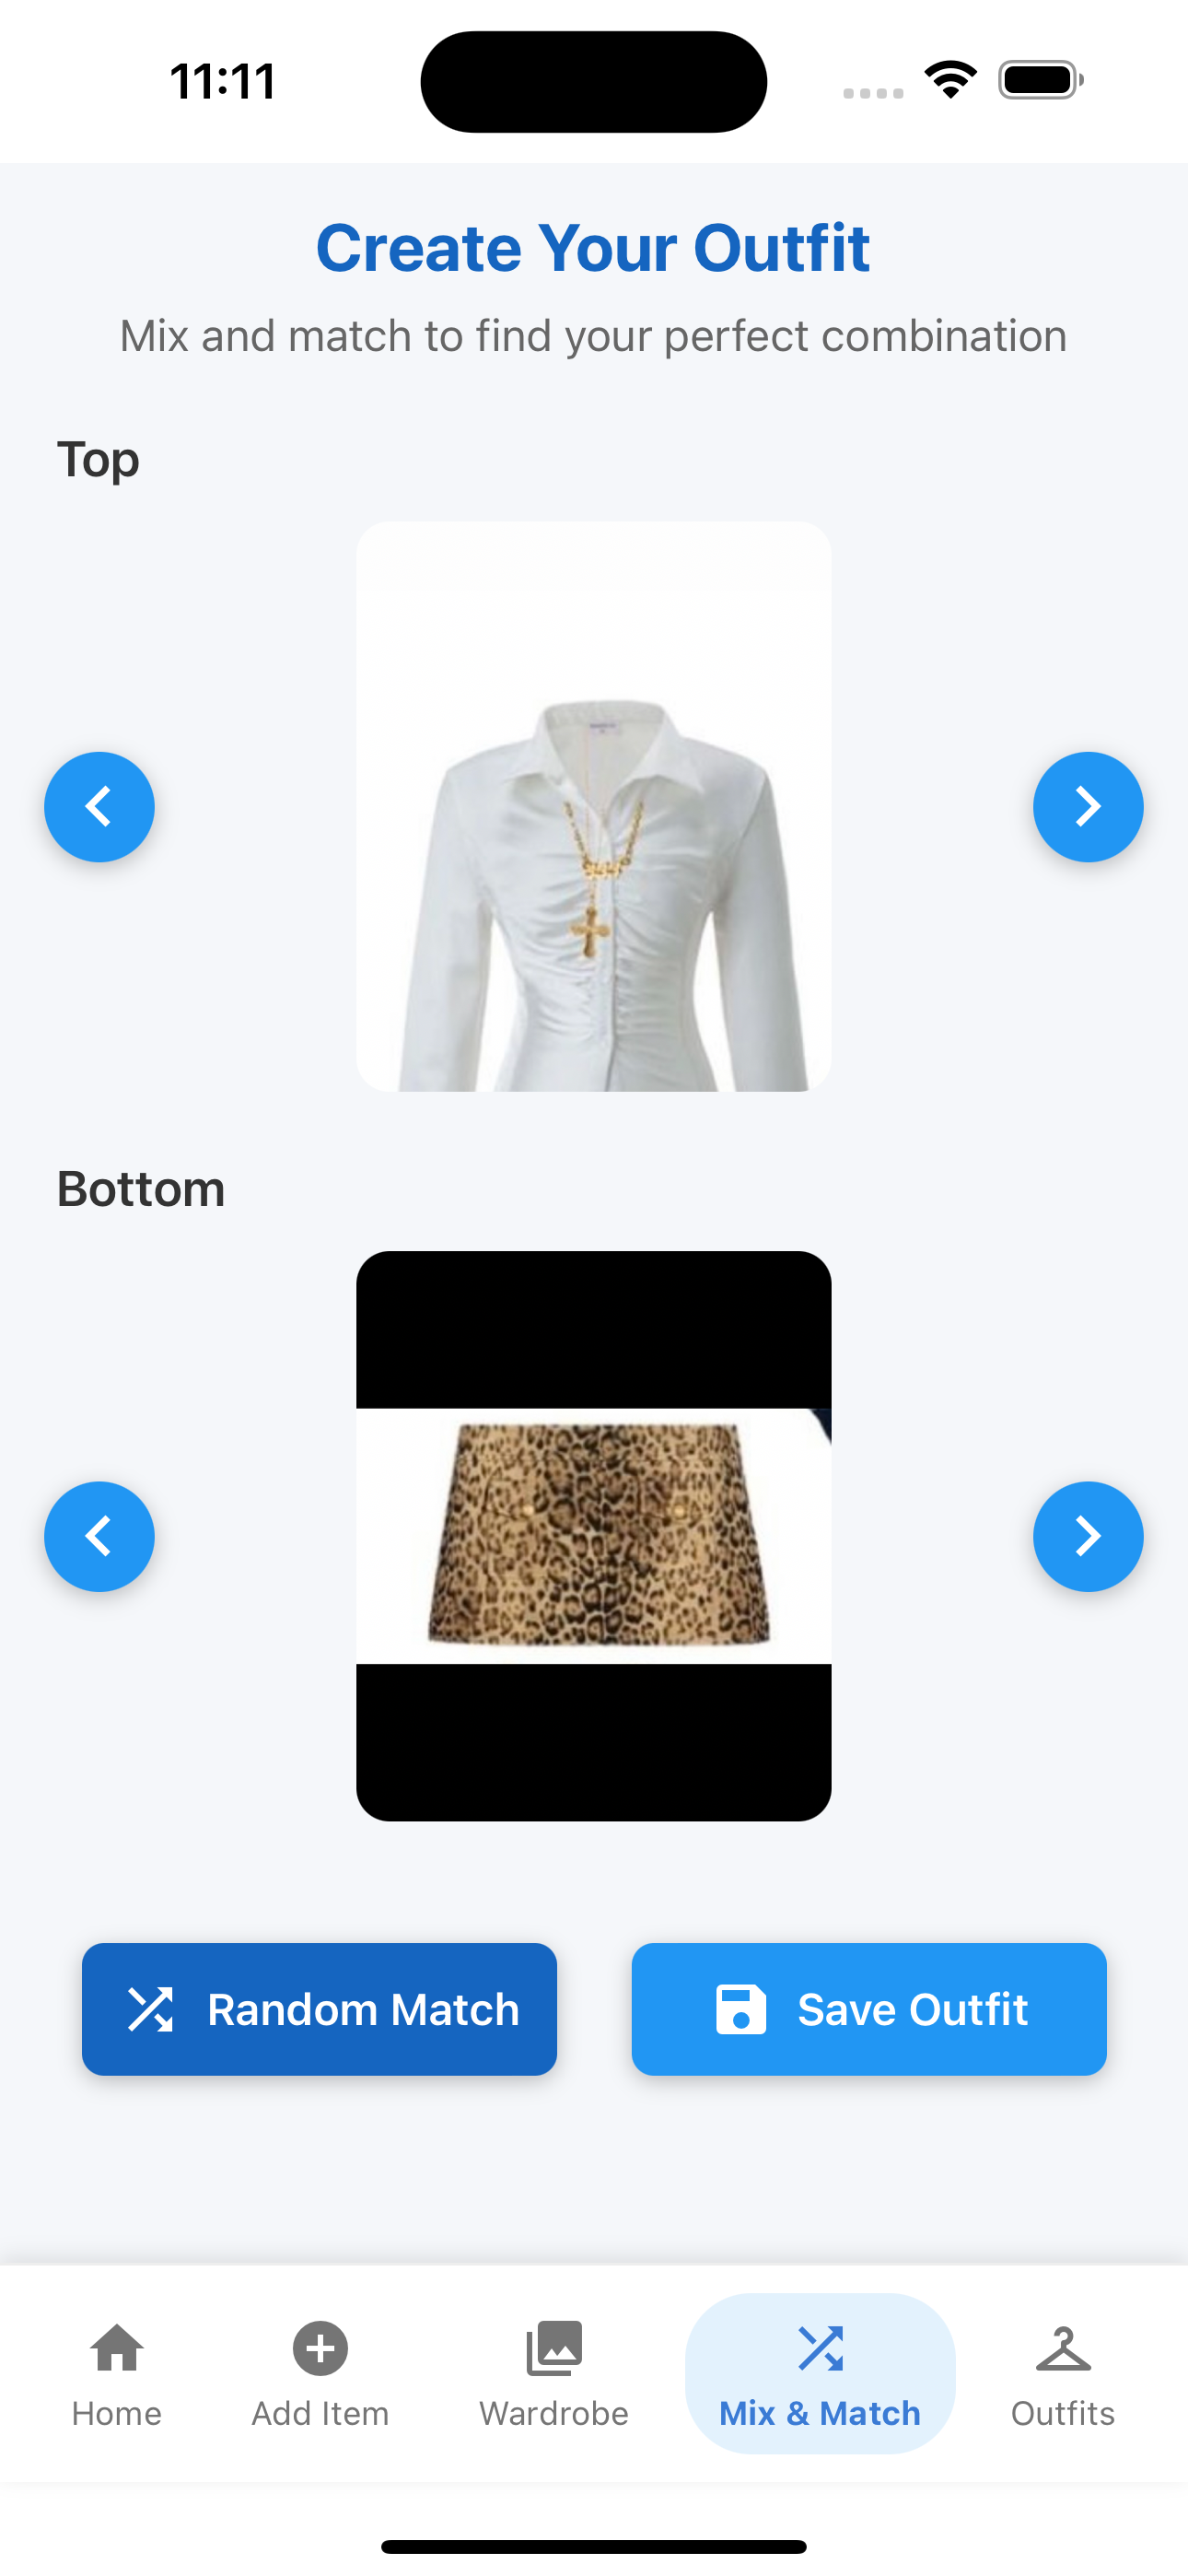
\includegraphics[width=0.3\textwidth]{exampleis-master/figures/mixandmatch.png}}
    \qquad % Adds horizontal spacing between the images
    % Second Subfloat: Outfit Screen
    \subfloat[Outfit screen - users can view and manage saved outfits.\label{fig:outfit_screen}]
    {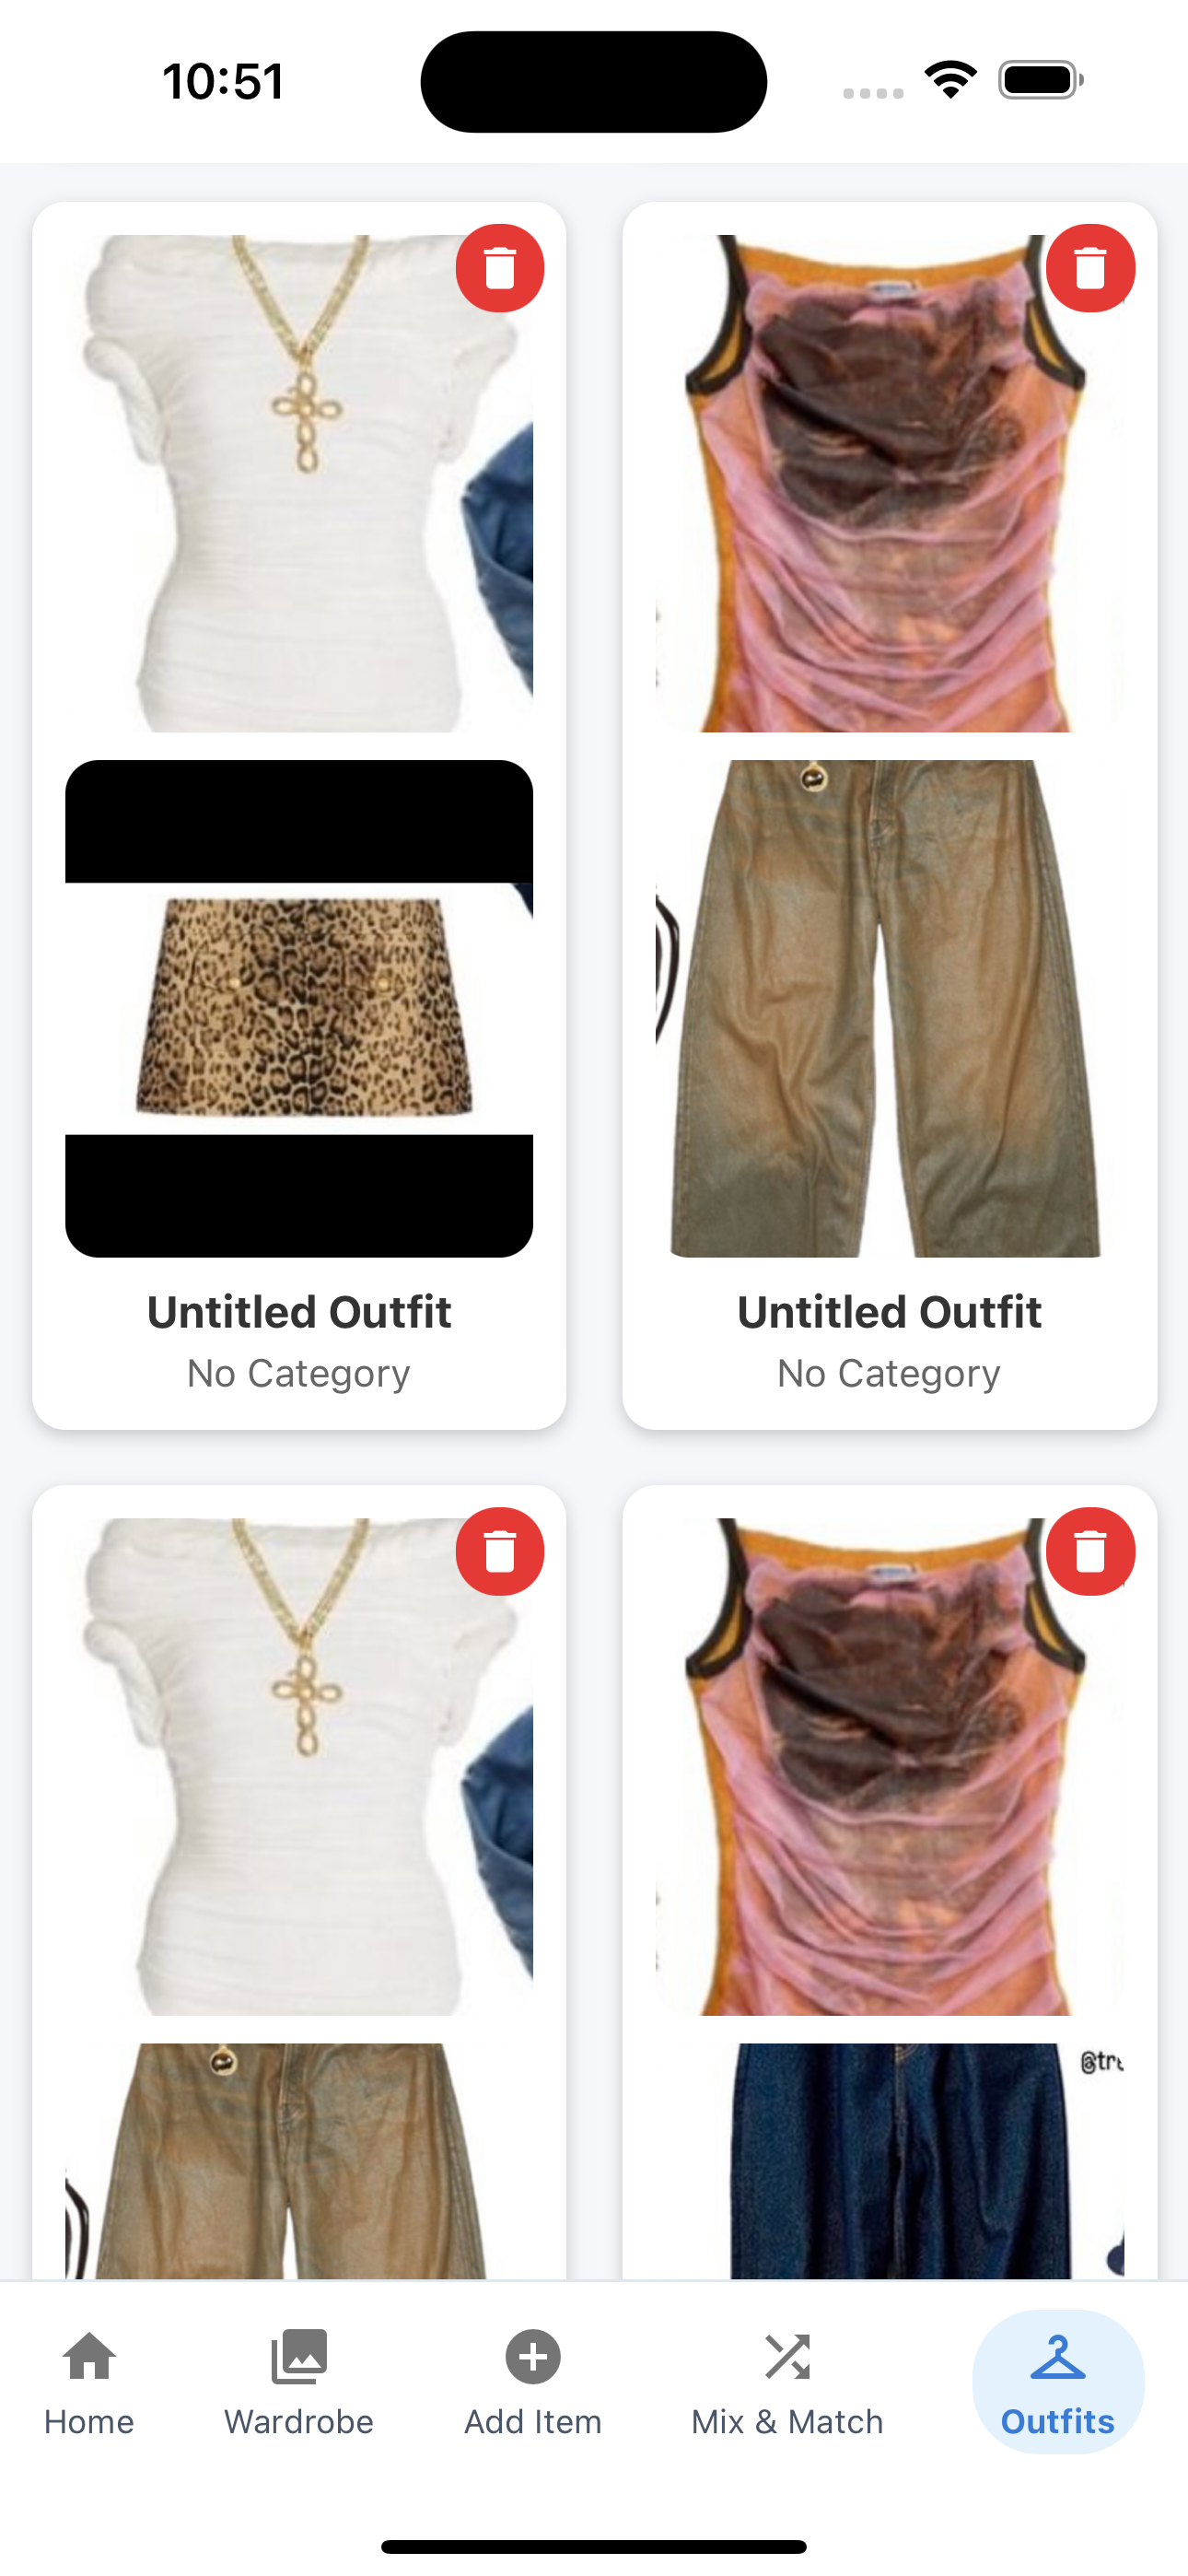
\includegraphics[width=0.3\textwidth]{exampleis-master/figures/outfitscreen2.png}}
    \caption{Outfit creation and saving: users can browse their saved outfits in the mix and match screen and view saved outfits in the outfit screen.}
    \label{fig:wardrobe_outfit_flow}
\end{figure}

By integrating categorization, interactive browsing, and dynamic previews, My Digital Wardrobe provides an intuitive wardrobe management experience. Users can filter through their collection, mix and match outfits, and save preferred combinations for future reference. Figure \ref{fig:mixandmatch_screen} shows how categorized wardrobe items are displayed and selected, while Figure \ref{fig:outfit_screen} demonstrates the saved outfit interface.
With images securely stored and categorized, the next step is allowing users to upload and manage their wardrobe items effectively. 
These features streamline wardrobe organization, making it easy for users to manage and experiment with their clothing selections.

\section{Component Communication}

\textit{My Digital Wardrobe} is built as a collection of interconnected components, each responsible for a specific function within the app. These components handle everything from user authentication to outfit creation, working together to create an intuitive experience. In the previous section we discussed how  certain implementations work along with visual aid, this section provides a step-by-step walkthrough of how the components communicate behind the scenes, ensuring that every action a user takes leads to a meaningful response.

At the heart of the app’s functionality is the way components interact with Firebase. Each time a user logs in, uploads an image, or saves an outfit, data is sent to Firebase services, which stores and manages this information. Expo Router handles navigation, directing users to the appropriate screens based on their actions. This structure ensures that the app remains responsive and dynamic, allowing users to interact with their wardrobe in a natural way.

\begin{table}[h]
    \centering
    \begin{tabular}{|l|l|p{5cm}|}
        \hline
        \textbf{File} & \textbf{Interacts With} & \textbf{Purpose} \\
        \hline
        \texttt{index.js} & \texttt{firebase.js} & Initializes authentication and manages user navigation based on authentication status. \\
        \hline
        \texttt{firebaseUpload.js} & \texttt{firebase.js}, \texttt{upload.js} & Handles image uploads to Firebase Storage and metadata storage in Firestore. \\
        \hline
        \texttt{upload.js} & \texttt{firebaseUpload.js} & Provides the interface for selecting, uploading, and categorizing wardrobe items. \\
        \hline
        \texttt{GalleryScreen.js} & \texttt{firestore.js}, \texttt{OutfitScreen.js} & Displays categorized wardrobe items fetched from Firestore. \\
        \hline
        \texttt{OutfitScreen.js} & \texttt{firebase.js}, \texttt{outfitfirestore.js} & Allows users to view saved outfits or create new outfits by mixing and matching wardrobe items. \\
        \hline
        \texttt{MixAndMatchScreen.js} & \texttt{outfitfirestore.js} & Enables users to select tops and bottoms, check color coordination, and save custom outfits to Firestore. \\
        \hline
    \end{tabular}
    \caption{Component interactions in my digital wardrobe}
    \label{tab:component_communication}
\end{table}

\subsection{Communication Flow}
The user journey begins the moment they open the app. When the app launches, \texttt{index.js} checks whether the user is already logged in. If authentication is successful, they are directed to the \texttt{HomeScreen} as shown in Figure \ref{fig:home}, where they can access different features. If not, they are taken to \texttt{LoginScreen} from Figure \ref{fig:login}, where they must enter their credentials before proceeding.
Once authenticated, the home screen serves as the main entry point. From here, users can choose to upload new clothing items, browse their wardrobe, mix and match outfits, or review previously saved outfits. Each screen is connected to the others through navigation events, ensuring that users can move fluidly between different sections.

When a user selects the option to add a new item, they are taken to \texttt{UploadScreen} in Figure \ref{fig:upload_screen}. This screen allows them to pick images from their device’s gallery and assign them to a category—either “Tops” or “Bottoms.” The selected image is then uploaded to Firebase Storage, while metadata such as category and upload timestamp is stored in Firestore.

The upload process happens in the background, ensuring that users can continue interacting with the app without delays. Once the upload is complete, the wardrobe is updated, and the new item appears in \texttt{GalleryScreen} from Figure \ref{fig:wardrobe_screen}, where it is sorted based on its assigned category.


In \texttt{GalleryScreen}, users can see all the clothing items they have uploaded, organized into their respective categories. When they tap on an item, it is highlighted, indicating that it has been selected. If they wish to create an outfit, they can navigate to \texttt{MixAndMatchScreen} from Figure \ref{fig:mixandmatch_screen}, where they can pair different tops and bottoms to find the best combination.

This screen presents a scrolling view of wardrobe items, allowing users to browse through their collection. They can manually select items or use the randomization feature to generate outfit suggestions. This interaction mimics the experience of flipping through a physical wardrobe, making outfit selection both simple and engaging.

Once a user has found a combination they like, they can save the outfit. This action sends the selected top and bottom to Firestore, where it is stored as a new outfit entry. Saved outfits can be accessed later in OutfitScreen in Figure \ref{fig:outfit_screen}, where users can review, edit, or delete them.

The outfit screen presents saved combinations in a structured layout, ensuring that users can quickly browse their past selections. If they decide to modify an outfit, they can return to MixAndMatchScreen in Figure \ref{fig:mixandmatch_screen} and make adjustments. This creates a continuous loop, where users can experiment with different styles, save their favorites, and revisit them whenever needed.


Every screen in My Digital Wardrobe is designed to respond to user actions, creating an easy interaction flow. Table \ref{tab:component_communication} shows a short summary of these interactions.



%!TEX root = ../username.tex
\chapter{Conclusion}
\label{chap:Chaptert6}
The development of \textit{My Digital Wardrobe} has focused on creating an accessible and efficient tool for wardrobe management. The app provides users with a structured way to upload, categorize, and explore their clothing collections, ensuring a more organized approach to outfit planning. Throughout the development process, several challenges emerged, particularly in balancing functionality with ease of use. While the app successfully integrates cloud storage and real-time accessibility, certain design limitations and missing features highlight opportunities for future improvement.

\section{Design Principles and Challenges}
A key design goal for My Digital Wardrobe was to create a clean, user-friendly interface that simplifies wardrobe organization. The login and upload screens were developed with a focus on clarity, using well-defined action buttons and recognizable icons to ensure intuitive navigation. The app follows a minimalist design, allowing users to upload and browse clothing items easily. However, some areas of the app feel visually cluttered, particularly the Wardrobe Screen and Outfit Screen, where multiple clothing items are displayed at once. While this does not significantly impact usability, refining the layout to improve spacing and readability will enhance the overall experience.

One of the most notable limitations is categorization. The current system requires users to manually assign clothing items to predefined categories, which are currently limited to tops and bottoms. This restriction reduces the app’s effectiveness as a wardrobe management tool, as users with diverse clothing collections cannot fully organize their wardrobe. Expanding the categorization system to include coats, jackets, dresses, accessories, and seasonal items is a necessary next step in making the app more comprehensive.

User testing was conducted using Expo, allowing the app to be deployed on different devices without extensive setup. This made testing quick and efficient, ensuring that the app could be evaluated across multiple platforms without delays. Testing confirmed that the app’s core features function as intended, with smooth navigation and a responsive interface. To simulate real wardrobe items, three tops and three bottoms were selected from Pinterest, a platform where users browse and save images, including fashion inspiration. Using Pinterest images helped create a realistic testing scenario, reflecting how users might upload and organize their own clothing collections.

While the fundamental features work well, personalization remains an area for improvement. Currently, the app provides a structured way to manage clothing, but it does not adapt to individual user preferences. Future updates will introduce customization features, such as the ability to tag favorite items, track frequently worn outfits, and receive outfit recommendations based on past selections. These enhancements will help tailor the experience to each user’s unique style, making the app more engaging and practical as a daily styling tool.

By addressing these challenges, My Digital Wardrobe will continue to refine its design while expanding its capabilities, ensuring a more user-focused wardrobe management experience.

\section{Future Enhancements}
To further enhance the functionality of My Digital Wardrobe, several key improvements are planned, with a focus on expanding categorization, streamlining automation, enhancing personalization, and enabling multi-platform accessibility.

One of the top priorities is expanding the categorization system beyond basic classifications like tops and bottoms. Future updates will introduce coats, jackets, accessories, and seasonal items, providing a more structured way to organize a wider range of clothing.

To enhance this process, the app will integrate machine learning (ML) for automatic classification, eliminating the need for manual categorization. An ML model will be trained on diverse clothing images to accurately recognize item types, streamlining uploads and reducing user effort. This implementation will involve dataset training, optimizing classification accuracy, and ensuring seamless integration with Firebase.

Another planned enhancement is web deployment, making My Digital Wardrobe accessible beyond mobile devices. While the current version is built using React Native and Expo, the web version will require adapting the interface for larger screens and optimizing performance for desktop use. Ensuring that wardrobe data remains synchronized across both mobile and web platforms will be a key challenge, necessitating refinements in Firebase’s authentication and storage mechanisms.

Personalization will also be a major focus moving forward. The app will introduce customization features that allow users to tag favorite items, track frequently worn outfits, and set wardrobe preferences. Additionally, an outfit recommendation system will be explored, utilizing stored wardrobe data to suggest clothing combinations based on past selections and user-defined preferences. These features will enhance usability by tailoring the experience to individual styling habits rather than simply serving as a digital catalog.

With these enhancements, My Digital Wardrobe will evolve into a more intelligent, adaptable, and widely accessible wardrobe management tool. Expanding categorization, automating classification, and enabling web deployment will ensure that users have a full experience across devices while reducing manual effort. By refining personalization features and implementing outfit recommendations, the app will move beyond basic wardrobe organization, offering a more interactive and user-focused styling experience. As development progresses, the focus will remain on optimizing usability, streamlining functionality, and expanding platform compatibility.



%\input{chapters/chapter6}
%\input{chapters/chapter7}
%\input{conclusion}

%%%%%%%%%%%%%%%%%%%%%%%%%%%%%%%%%%%%%%%%%%%%%%%%%%%%%%%
%
%  This section starts the back matter. The back matter includes appendices, indicies, and the
%  bibliography
%
%%%%%%%%%%%%%%%%%%%%%%%%%%%%%%%%%%%%%%%%%%%%%%%%%%%%%%%

\backmatter

% %!TEX root = ../username.tex
% %%%%%%%%%%%%%%%%%%%%%%%%%%%%%%%%%%%%%%%%%%%%%%%%%%%%%%%%%%%%%%%%
% % Contents: Math typesetting with LaTeX
% % $Id: math.tex,v 1.3 2005/05/21 02:03:43 jonb Exp $
% %%%%%%%%%%%%%%%%%%%%%%%%%%%%%%%%%%%%%%%%%%%%%%%%%%%%%%%%%%%%%%%%%

% \chapter{Typesetting Mathematical Formulae}\label{math}
% \begin{intro}
%   This appendix is taken from \citet{ophs03} under the GNU open-source documentation license. This appendix addresses the main strength
%   of \TeX{}: mathematical typesetting. But be warned, this appendix
%   only scratches the surface. While the things explained here are
%   sufficient for many people, don't despair if you can't find a
%   solution to your mathematical typesetting needs here. It is highly likely
%   that your problem is addressed in \AmS-\LaTeX{}%
%   \footnote{\texttt{CTAN:/tex-archive/macros/latex/packages/amslatex}}
%   or some other package.
% \end{intro}
  
% \section{General}

% \LaTeX{} has a special mode for typesetting mathematics\index{mathematics}.
% Mathematical text within a paragraph is entered between \verb|\(|\index{\(@\verb+\(+}
% and \verb|\)|\index{\)@\verb+\)+}, %$
% between \texttt{\$} and \texttt{\$} or between
% \verb|\begin{|{math}\verb|}| and \verb|\end{math}|.\index{formulae}

% \begin{singlespace}
% \begin{example}
% Add $a$ squared and $b$ squared 
% to get $c$ squared. Or, using 
% a more mathematical approach:
% $c^{2}=a^{2}+b^{2}$
% \end{example}
% \end{singlespace}

% \begin{singlespace}
% \begin{example}
% \TeX{} is pronounced as 
% $\tau\epsilon$.\\[6pt]
% 100~m$^{3}$ of water\\[6pt]
% This comes from my $\heartsuit$
% \end{example}
% \end{singlespace}

% It is preferable to \emph{display} larger mathematical equations or formulae,
% rather than to typeset them on separate lines. This means you enclose them
% in \verb|\[| \index{\[@\verb+\[+} and \verb|\]| \index{\]@\verb+\]+} or between
% \verb|\begin{|displaymath\index{displaymath}\verb|}| and
%   \verb|\end{displaymath}|.  This produces formulae which are not
% numbered. If you want \LaTeX{} to number them, you can use the
% equation\index{equation} environment.


% \begin{singlespace}
% \begin{example}
% Add $a$ squared and $b$ squared 
% to get $c$ squared. Or, using 
% a more mathematical approach:
% \begin{displaymath}
% c^{2}=a^{2}+b^{2}
% \end{displaymath}
% And just one more line.
% \end{example}
% \end{singlespace}

% You can reference an equation with \ic{label} and \ic{ref}

% \begin{singlespace}
% \begin{example}
% \begin{equation} \label{eq:eps}
% \epsilon > 0
% \end{equation}
% From (\ref{eq:eps}), we gather 
% \ldots
% \end{example}
% \end{singlespace}

% Note that expressions will be typeset in a different style if displayed:

% \begin{singlespace}
% \begin{example}
% $\lim_{n \to \infty} 
% \sum_{k=1}^n \frac{1}{k^2} 
% = \frac{\pi^2}{6}$
% \end{example}
% \end{singlespace}
% \begin{singlespace}
% \begin{example}
% \begin{displaymath}
% \lim_{n \to \infty} 
% \sum_{k=1}^n \frac{1}{k^2} 
% = \frac{\pi^2}{6}
% \end{displaymath}
% \end{example}
% \end{singlespace}

% There are differences between \emph{math mode} and \emph{text mode}. For
% example, in \emph{math mode}: 

% \begin{enumerate}

% \item Most spaces and linebreaks do not have any significance, as all spaces
% either are derived logically from the mathematical expressions or
% have to be specified using special commands such as \verb|\,| \index{''\,@\verb+\,+}, \ic{quad}, or \ic{qquad}.
 
% \item Empty lines are not allowed. Only one paragraph per formula.

% \item Each letter is considered to be the name of a variable and will be
% typeset as such. If you want to typeset normal text within a formula
% (normal upright font and normal spacing) then you have to enter the
% text using the \verb|\textrm{...}| commands.
% \end{enumerate}


% \begin{singlespace}
% \begin{example}
% \begin{equation}
% \forall x \in \mathbf{R}:
% \qquad x^{2} \geq 0
% \end{equation}
% \end{example}
% \end{singlespace}

% \begin{singlespace}
% \begin{example}
% \begin{equation}
% x^{2} \geq 0\qquad
% \textrm{for all }x\in\mathbf{R}
% \end{equation}
% \end{example}
% \end{singlespace}

% Mathematicians can be very fussy about which symbols are used:
% it would be conventional here to use `blackboard bold\index{blackboard bold}',
% bold symbols\index{bold symbols} which is obtained using \ic{mathbb} from the
% package \ip{amsfonts} or \ip{amssymb}.

% \ifx\mathbb\undefined\else
% The last example becomes
% \begin{singlespace}
% \begin{example}
% \begin{displaymath}
% x^{2} \geq 0\qquad
% \textrm{for all }x\in\mathbb{R}
% \end{displaymath}
% \end{example}
% \end{singlespace}
% \fi

% \section{Grouping in Math Mode}

% Most math mode commands act only on the next character. So if you
% want a command to affect several characters, you have to group them
% together using curly braces: \verb|{...}|.

% \begin{singlespace}
% \begin{example}
% \begin{equation}
% a^x+y \neq a^{x+y}
% \end{equation}
% \end{example}
% \end{singlespace}
 
% \section{Building Blocks of a Mathematical Formula}

% In this section, the most important commands used in mathematical
% typesetting will be described. Take a look at \citet{kd03} for a detailed list of commands for typesetting
% mathematical symbols.

% \textbf{Lowercase Greek letters\index{Greek letters}} are entered as \verb|\alpha|,
%  \verb|\beta|, \verb|\gamma|, \ldots, uppercase letters
% are entered as \verb|\Gamma|, \verb|\Delta|, \ldots\footnote{There is no
%   uppercase Alpha defined in \LaTeXe{} because it looks the same as a
%   normal roman A. Once the new math coding is done, things will
%   change.} 

% \begin{singlespace}
% \begin{example}
% $\lambda,\xi,\pi,\mu,\Phi,\Omega$
% \end{example}
% \end{singlespace}
 
% \textbf{Exponents and Subscripts} can be specified using\index{exponent}\index{subscript}
% the \verb|^|\index{^@\verb+^+} and the \verb|_|\index{_@\verb+_+} character.

% \begin{singlespace}
% \begin{example}
% $a_{1}$ \qquad $x^{2}$ \qquad
% $e^{-\alpha t}$ \qquad
% $a^{3}_{ij}$\\
% $e^{x^2} \neq {e^x}^2$
% \end{example}
% \end{singlespace}

% The \textbf{square root\index{square root}} is entered as \ic{sqrt}, the
% $n^\mathrm{th}$ root is generated with \verb|\sqrt[|$n$\verb|]|. The size of
% the root sign is determined automatically by \LaTeX. If just the sign
% is needed, use \ic{surd}.

% \begin{singlespace}
% \begin{example}
% $\sqrt{x}$ \qquad 
% $\sqrt{ x^{2}+\sqrt{y} }$ 
% \qquad $\sqrt[3]{2}$\\[3pt]
% $\surd[x^2 + y^2]$
% \end{example}
% \end{singlespace}

% The commands \ic{overline} and \ic{underline} create
% \textbf{horizontal lines} directly over or under an expression.
% \index{horizontal!line}

% \begin{singlespace}
% \begin{example}
% $\overline{m+n}$
% \end{example}
% \end{singlespace}

% The commands \ic{overbrace} and \ic{underbrace} create
% long \textbf{horizontal braces} over or under an expression.
% \index{horizontal!brace}

% \begin{singlespace}
% \begin{example}
% $\underbrace{ a+b+\cdots+z }_{26}$
% \end{example}
% \end{singlespace}

% \index{mathematical!accents} To add mathematical accents such as small
% arrows or {tilde} signs to variables, you can use the commands
% given in \citet{kd03}.  Wide hats and
% tildes covering several characters are generated with \ic{widetilde}
% and \ic{widehat}.  The \verb|'|\index{'@\verb+'+} symbol gives a
% prime\index{prime}.
% % a dash is --

% \begin{singlespace}
% \begin{example}
% \begin{displaymath}
% y=x^{2}\qquad y'=2x\qquad y''=2
% \end{displaymath}
% \end{example}
% \end{singlespace}

% \textbf{Vectors}\index{vectors} often are specified by adding a small
% arrow symbol\index{arrow symbols} on top of a variable. This is done with the
% \ic{vec} command. The two commands \ic{overrightarrow} and
% \ic{overleftarrow} are useful to denote the vector from $A$ to $B$.

% \begin{singlespace}
% \begin{example}
% \begin{displaymath}
% \vec a\quad\overrightarrow{AB}
% \end{displaymath}
% \end{example}
% \end{singlespace}

% Names of log-like functions are often typeset in an upright
% font and not in italic like variables. Therefore \LaTeX{} supplies the
% following commands to typeset the most important function names:
% \index{mathematical!functions}

% \begin{singlespace}
% \begin{verbatim}
% \arccos   \cos    \csc   \exp   \ker     \limsup  \min   \sinh
% \arcsin   \cosh   \deg   \gcd   \lg      \ln      \Pr    \sup
% \arctan   \cot    \det   \hom   \lim     \log     \sec   \tan
% \arg      \coth   \dim   \inf   \liminf  \max     \sin   \tanh
% \end{verbatim}
% \end{singlespace}

% \begin{singlespace}
% \begin{example}
% \[\lim_{x \rightarrow 0}
% \frac{\sin x}{x}=1\]
% \end{example}
% \end{singlespace}

% For the modulo function\index{modulo function}, there are two commands: \ic{bmod} for the
% binary operator ``$a \bmod b$'' and \ic{pmod}
% for expressions
% such as ``$x\equiv a \pmod{b}$.''

% A built-up \textbf{fraction\index{fraction}} is typeset with the
% \ic{frac}\verb|{...}{...}| command.
% Often the slashed form $1/2$ is preferable, because it looks better
% for small amounts of `fraction material.'

% \begin{singlespace}
% \begin{example}
% $1\frac{1}{2}$~hours
% \begin{displaymath}
% \frac{ x^{2} }{ k+1 }\qquad
% x^{ \frac{2}{k+1} }\qquad
% x^{ 1/2 }
% \end{displaymath}
% \end{example}
% \end{singlespace}

% To typeset binomial coefficients or similar structures, you can use
% either the command \linebreak \ic{binom}\{\emph{num}\}\{\emph{denom}\} or \ic{genfrac}\{\emph{ldelim}\}\{\emph{rdelim}\}\{\emph{thickness}\}\{\emph{style}\}\{\emph{num}\}\{\emph{denom}\}. The second command can be used to produce customized fraction like output and more information can be found in \citet{mgbcr04}.

% \begin{singlespace}
% \begin{example}
% \begin{displaymath}
% \binom{n}{k}\qquad 
% \genfrac{}{}{0pt}{}{x}{y+2}
% \end{displaymath}
% \end{example}
% \end{singlespace}
 
% \medskip

% The \textbf{integral operator\index{integral operator}} is generated with \ic{int}, the
% \textbf{sum operator\index{sum operator}} with \ic{sum}. The upper and lower limits
% are specified with~\verb|^|\index{^@\verb+^+} and~\verb|_|\index{_@\verb+_+} like subscripts and superscripts.

% \begin{singlespace}
% \begin{example}
% \begin{displaymath}
% \sum_{i=1}^{n} \qquad
% \int_{0}^{\frac{\pi}{2}} \qquad
% \end{displaymath}
% \end{example}
% \end{singlespace}

% For \textbf{braces\index{braces}} and other delimiters\index{delimiters}, there exist all
% types of symbols in \TeX{} (e.g.~$[\;\langle\;\|\;\updownarrow$).
% Round and square braces can be entered with the corresponding keys,
% curly braces with \verb|\{|, all other delimiters are generated with
% special commands (e.g.~\verb|\updownarrow|). For a list of all
% delimiters available, check \citet{kd03}.

% \begin{singlespace}
% \begin{example}
% \begin{displaymath}
% {a,b,c}\neq\{a,b,c\}
% \end{displaymath}
% \end{example}
% \end{singlespace}

% If you put the command \ic{left} in front of an opening delimiter or
% \ic{right} in front of a closing delimiter, \TeX{} will automatically
% determine the correct size of the delimiter. Note that you must close
% every \ic{left} with a corresponding \ic{right}, and that the size is
% determined correctly only if both are typeset on the same line. If you
% don't want anything on the right, use the invisible `\verb|\right .|\index{commands!right@\verb+right .+}'!

% \begin{singlespace}
% \begin{example}
% \begin{displaymath}
% 1 + \left( \frac{1}{ 1-x^{2} }
%     \right) ^3
% \end{displaymath}
% \end{example}
% \end{singlespace}

% In some cases it is necessary to specify the correct size of a
% mathematical delimiter\index{mathematical!delimiter} by hand,
% which can be done using the commands \ic{big}, \ic{Big}, \ic{bigg} and
% \ic{Bigg} as prefixes to most delimiter commands.\footnote{These
%   commands do not work as expected if a size changing command has been
%   used, or the \texttt{11pt} or \texttt{12pt} option has been
%   specified.  Use the exscale\index{exscale} or amsmath\index{amsmath} packages to
%   correct this behaviour.}

% \begin{singlespace}
% \begin{example}
% $\Big( (x+1) (x-1) \Big) ^{2}$\\
% $\big(\Big(\bigg(\Bigg($\quad
% $\big\}\Big\}\bigg\}\Bigg\}$\quad
% $\big\|\Big\|\bigg\|\Bigg\|$
% \end{example}
% \end{singlespace}

% To enter \textbf{three dots\index{three dots}} into a formula, you can use several
% commands. \ic{ldots} typesets the dots on the baseline, \ic{cdots}
% sets them centered. Besides that, there are the commands \ic{vdots} for
% vertical and \ic{ddots} for diagonal dots\index{diagonal dots}.\index{vertical
%   dots}\index{horizontal!dots} You can find another example in section~\ref{sec:vert}.

% \begin{singlespace}
% \begin{example}
% \begin{displaymath}
% x_{1},\ldots,x_{n} \qquad
% x_{1}+\cdots+x_{n}
% \end{displaymath}
% \end{example}
% \end{singlespace}
 
% \section{Math Spacing}

% \index{math spacing} If the spaces within formulae chosen by \TeX{}
% are not satisfactory, they can be adjusted by inserting special
% spacing commands. There are some commands for small spaces: \verb|\,| \index{\,@\verb+\,+} for
% $\frac{3}{18}\:\textrm{quad}$ (\demowidth{0.166em}), \verb|\:| \index{\:@\verb+\:+} for $\frac{4}{18}\:
% \textrm{quad}$ (\demowidth{0.222em}) and \verb|\;| \index{\;@\verb+\;+} for $\frac{5}{18}\:
% \textrm{quad}$ (\demowidth{0.277em}).  The escaped space character
% \verb*.\ . generates a medium sized space and \ic{quad}
% (\demowidth{1em}) and \ic{qquad} (\demowidth{2em}) produce large
% spaces. The size of a quad corresponds to the width of the
% character `M' of the current font.  The \verb|\!|\index{"\"!@\texttt{\bs"!}} command produces a
% negative space of $-\frac{3}{18}\:\textrm{quad}$ (\demowidth{0.166em}).

% \begin{singlespace}
% \begin{example}
% \newcommand{\rd}{\mathrm{d}}
% \begin{displaymath}
% \int\!\!\!\int_{D} g(x,y)
%   \, \rd x\, \rd y 
% \end{displaymath}
% instead of 
% \begin{displaymath}
% \int\int_{D} g(x,y)\rd x \rd y
% \end{displaymath}
% \end{example}
% \end{singlespace}
% Note that `d' in the differential is conventionally set in roman.

% \AmS-\LaTeX{} provides another way for fine tuning
% the spacing between multiple integral signs,
% namely the \ic{iint}, \ic{iiint}, \ic{iiiint}, and \ic{idotsint} commands.
% With the \ip{amsmath} package loaded, the above example can be
% typeset this way:

% \begin{singlespace}
% \begin{example}
% \newcommand{\rd}{\mathrm{d}}
% \begin{displaymath}
% \iint_{D} \, \rd x \, \rd y
% \end{displaymath}
% \end{example}
% \end{singlespace}

% See the electronic document testmath.tex (distributed with
% \AmS-\LaTeX) or Chapter 8 of ``The LaTeX Companion''\footnote{
% available at \texttt{CTAN:/tex-archive/info/ch8.*}.} for further details.

% \section{Vertically Aligned Material}
% \label{sec:vert}

% To typeset \textbf{arrays}, use the \texttt{array}\index{array} environment. It works
% somewhat similar to the \texttt{tabular} environment. The \verb|\\| command is
% used to break the lines.

% \begin{singlespace}
% \begin{example}
% \begin{displaymath}
% \mathbf{X} =
% \left( \begin{array}{ccc}
% x_{11} & x_{12} & \ldots \\
% x_{21} & x_{22} & \ldots \\
% \vdots & \vdots & \ddots
% \end{array} \right)
% \end{displaymath}
% \end{example}
% \end{singlespace}

% The \texttt{array}\index{array} environment can also be used to typeset expressions which have one
% big delimiter by using a ``\verb|.|'' as an invisible right\index{commands!right@\verb+right .+} 
% delimiter:

% \begin{singlespace}
% \begin{example}
% \begin{displaymath}
% y = \left\{ \begin{array}{ll}
%  a & \textrm{if $d>c$}\\
%  b+x & \textrm{in the morning}\\
%  l & \textrm{all day long}
%   \end{array} \right.
% \end{displaymath}
% \end{example}
% \end{singlespace}


% For formulae running over several lines or for equation systems\index{equation systems},
% you can use the environments \texttt{eqnarray}\index{eqnarray}, and \verb|eqnarray*|
% instead of \texttt{equation}. In \texttt{eqnarray} each line gets an
% equation number. The \verb|eqnarray*| does not number anything.

% The \texttt{eqnarray} and the \verb|eqnarray*| environments work like
% a 3-column table of the form \verb|{rcl}|, where the middle column can
% be used for the equal sign or the not-equal sign. Or any other sign
% you see fit. The \verb|\\| command breaks the lines.

% \begin{singlespace}
% \begin{example}
% \begin{eqnarray}
% f(x) & = & \cos x     \\
% f'(x) & = & -\sin x   \\
% \int_{0}^{x} f(y)dy &
%  = & \sin x
% \end{eqnarray}
% \end{example}
% \end{singlespace}

% \noindent Notice that the space on either side of the 
% the equal signs is rather large. It can be reduced by setting
% \verb|\setlength\arraycolsep{2pt}|, as in the next example.

% \index{long equations} \textbf{Long equations} will not be
% automatically divided into neat bits.  The author has to specify
% where to break them and how much to indent. The following two methods
% are the most common ones used to achieve this.

% \begin{singlespace}
% \begin{example}
% {\setlength\arraycolsep{2pt}
% \begin{eqnarray}\notag
% \sin x & = & x -\frac{x^{3}}{3!}
%      +\frac{x^{5}}{5!}-{}
%                    \\\notag
%  & & {}-\frac{x^{7}}{7!}+{}\cdots
% \end{eqnarray}}
% \end{example}
% \end{singlespace}
% \pagebreak[1]

% \begin{singlespace}
% \begin{example}
% \begin{eqnarray}\notag
% \lefteqn{ \cos x = 1
%      -\frac{x^{2}}{2!} +{} }
%                    \\\notag
%  & & {}+\frac{x^{4}}{4!}
%      -\frac{x^{6}}{6!}+{}\cdots
% \end{eqnarray}
% \end{example}
% \end{singlespace}

% \enlargethispage{\baselineskip}

% \noindent The \ic{notag} command causes \LaTeX{} to not generate a number for
% this equation.

% It can be difficult to get vertically aligned equations to look right
% with these methods; the package amsmath\index{amsmath} provides a more
% powerful set of alternatives.

% \section{Math Font Size}

% \index{math font size} In math mode, \TeX{} selects the font size
% according to the context. Superscripts, for example, get typeset in a
% smaller font. If you want to typeset part of an equation in roman,
% don't use the \ic{textrm} command, because the font size switching
% mechanism will not work, as \verb|\textrm| temporarily escapes to text
% mode. Use \verb|\mathrm| instead to keep the size switching mechanism
% active. But pay attention, \ic{mathrm} will only work well on short
% items. Spaces are still not active and accented characters do not
% work.\footnote{The \AmS-\LaTeX{} package makes the textrm command
%   work with size changing.}

% \begin{singlespace}
% \begin{example}
% \begin{equation}
% 2^{\textrm{nd}} \quad 
% 2^{\mathrm{nd}}
% \end{equation}
% \end{example}
% \end{singlespace}

% Nevertheless, sometimes you need to tell \LaTeX{} the correct font
% size. In math mode, the font size is set with the four commands:
% \begin{center}
% {displaystyle}~($\displaystyle 123$),
% {textstyle}~($\textstyle 123$), 
% {scriptstyle}~($\scriptstyle 123$) and
% {scriptscriptstyle}~($\scriptscriptstyle 123$).
% \end{center}

% Changing styles also affects the way limits are displayed.

% \begin{singlespace}
% \begin{example}
% \begin{displaymath}
% \mathop{\mathrm{corr}}(X,Y)= 
%  \frac{\displaystyle 
%    \sum_{i=1}^n(x_i-\overline x)
%    (y_i-\overline y)} 
%   {\displaystyle\biggl[
%  \sum_{i=1}^n(x_i-\overline x)^2
% \sum_{i=1}^n(y_i-\overline y)^2
% \biggr]^{1/2}}
% \end{displaymath}    
% \end{example}
% \end{singlespace}
% % This is not a math accent, and no maths book would be set this way.
% % mathop gets the spacing right.

% \noindent This is one of those examples in which we need larger
% brackets than the standard \verb|\left[  \right]| provides.


% \section{Theorems, Laws, \ldots}

% When writing mathematical documents, you probably need a way to
% typeset ``Lemmas'', ``Definitions'', ``Axioms'' and similar
% structures. \LaTeX{} supports this with the command
% \begin{command}
% {newtheorem}\verb|{|\emph{name}\verb|}[|\emph{counter}\verb|]{|%
%          \emph{text}\verb|}[|\emph{section}\verb|]|
% \end{command}
% The \emph{name} argument, is a short keyword used to identify the
% ``theorem''. With the \emph{text} argument, you define the actual name
% of the ``theorem'' which will be printed in the final document.

% The arguments in square brackets are optional. They are both used to
% specify the numbering used on the ``theorem''. With the \emph{counter}
% argument you can specify the \emph{name} of a previously declared
% ``theorem''. The new ``theorem'' will then be numbered in the same
% sequence.  The \emph{section} argument allows you to specify the
% sectional unit within which you want your ``theorem'' to be numbered.

% After executing the {newtheorem} command in the preamble of your
% document, you can use the following command within the document.

% \begin{code}
% \verb|\begin{|\emph{name}\verb|}[|\emph{text}\verb|]|\\
% This is my interesting theorem\\
% \verb|\end{|\emph{name}\verb|}|     
% \end{code}

% This should be enough theory. The following examples will hopefully
% remove the final remains of doubt and make it clear that the
% \verb|\newtheorem| environment is way too complex to understand.

% \begin{singlespace}
% \begin{example}
% % definitions for the document
% % preamble
% \newtheorem{law}{Law}
% \newtheorem{jury}[law]{Jury}
% %in the document
% \begin{law} \label{law:box}
% Don't hide in the witness box
% \end{law}
% \begin{jury}[The Twelve]
% It could be you! So beware and
% see law~\ref{law:box}\end{jury}
% \begin{law}No, No, No\end{law}
% \end{example}
% \end{singlespace}

% The ``Jury'' theorem uses the same counter as the ``Law''
% theorem. Therefore it gets a number which is in sequence with
% the other ``Laws''. The argument in square brackets is used to specify 
% a title or something similar for the theorem.

% \begin{singlespace}
% \begin{example}
% \flushleft
% \newtheorem{mur}{Murphy}[section]
% \begin{mur}
% If there are two or more 
% ways to do something, and 
% one of those ways can result 
% in a catastrophe, then 
% someone will do it.\end{mur}
% \end{example}
% \end{singlespace}

% The ``Murphy'' theorem gets a number which is linked to the number of
% the current section. You could also use another unit, for example chapter or
% subsection.

% \section{Bold symbols}
% \index{bold symbols}

% It is quite difficult to get bold symbols in \LaTeX{}; this is 
% probably intentional as amateur typesetters tend to overuse them.
% The font change command \verb|\mathbf| gives bold letters, but these are
% roman (upright) whereas mathematical symbols are normally italic.
% There is a \ic{boldmath} command, but \emph{this can only be
% used outside mathematics mode}. It works for symbols too.

% \begin{singlespace}
% \begin{example}
% \begin{displaymath}
% \mu, M \qquad \mathbf{M} \qquad
% \mbox{\boldmath $\mu, M$}
% \end{displaymath}
% \end{example}
% \end{singlespace}

% \noindent
% Notice that the comma is bold too, which may not be what is required.

% The package \ip{amsbsy} (included by \ip{amsmath}) makes this much
% easier as it includes a \ic{boldsymbol} command.

% \ifx\boldsymbol\undefined\else
% \begin{singlespace}
% \begin{example}
% \begin{displaymath}
% \mu, M \qquad
% \boldsymbol{\mu}, \boldsymbol{M}
% \end{displaymath}
% \end{example}
% \end{singlespace}
% \fi

% \section{List of Mathematical Symbols}  \label{symbols}
 
% In the following tables, you find all the symbols normally accessible
% from \emph{math mode}.  

% %
% % Conditional Text in case the AMS Fonts are installed
% %
% \ifx\noAMS\relax To use the symbols listed in
% Tables~\ref{AMSD}--\ref{AMSNBR},\footnote{These tables were derived
%   from \texttt{symbols.tex} by David~Carlisle and subsequently changed
% extensively as suggested by Josef~Tkadlec.} the package
% \ip{amssymb} must be loaded in the preamble of the document and the
% AMS math fonts must be installed, on the system. If the AMS package and
% fonts are not installed, on your system, have a look at\\ 
% \texttt{CTAN:/tex-archive/macros/latex/required/amslatex}\fi
 
% \begin{table}[!ht]
% \caption{Math Mode Accents.}  \label{mathacc}
% \begin{symbols}{*4{cl}}
% \W{\hat}{a}     & \W{\check}{a} & \W{\tilde}{a} & \W{\acute}{a} \\
% \W{\grave}{a} & \W{\dot}{a} & \W{\ddot}{a}    & \W{\breve}{a} \\
% \W{\bar}{a} &\W{\vec}{a} &\W{\widehat}{A}&\W{\widetilde}{A}\\  
% \end{symbols}
% \end{table}
 
% \begin{table}[!ht]
% \caption{Lowercase Greek Letters.}
% \begin{symbols}{*4{cl}}
%  \X{\alpha}     & \X{\theta}     & \X{o}          & \X{\upsilon}  \\
%  \X{\beta}      & \X{\vartheta}  & \X{\pi}        & \X{\phi}      \\
%  \X{\gamma}     & \X{\iota}      & \X{\varpi}     & \X{\varphi}   \\
%  \X{\delta}     & \X{\kappa}     & \X{\rho}       & \X{\chi}      \\
%  \X{\epsilon}   & \X{\lambda}    & \X{\varrho}    & \X{\psi}      \\
%  \X{\varepsilon}& \X{\mu}        & \X{\sigma}     & \X{\omega}    \\
%  \X{\zeta}      & \X{\nu}        & \X{\varsigma}  & &             \\
%  \X{\eta}       & \X{\xi}        & \X{\tau} 
% \end{symbols}
% \end{table}

% \begin{table}[!ht]
% \caption{Uppercase Greek Letters.}
% \begin{symbols}{*4{cl}}
%  \X{\Gamma}     & \X{\Lambda}    & \X{\Sigma}     & \X{\Psi}      \\
%  \X{\Delta}     & \X{\Xi}        & \X{\Upsilon}   & \X{\Omega}    \\
%  \X{\Theta}     & \X{\Pi}        & \X{\Phi} 
% \end{symbols}
% \end{table}
% \clearpage 

% \begin{table}[!tbp]
% \caption{Binary Relations.}
% \bigskip
% You can produce corresponding negations by adding a \verb|\not| command
% as prefix to the following symbols.
% \begin{symbols}{*3{cl}}
%  \X{<}           & \X{>}           & \X{=}          \\
%  \X{\leq}or \verb|\le|   & \X{\geq}or \verb|\ge|   & \X{\equiv}     \\
%  \X{\ll}         & \X{\gg}         & \X{\doteq}     \\
%  \X{\prec}       & \X{\succ}       & \X{\sim}       \\
%  \X{\preceq}     & \X{\succeq}     & \X{\simeq}     \\
%  \X{\subset}     & \X{\supset}     & \X{\approx}    \\
%  \X{\subseteq}   & \X{\supseteq}   & \X{\cong}      \\
%  \X{\sqsubset}$^a$ & \X{\sqsupset}$^a$ & \X{\Join}$^a$    \\
%  \X{\sqsubseteq} & \X{\sqsupseteq} & \X{\bowtie}    \\
%  \X{\in}         & \X{\ni}, \verb|\owns|  & \X{\propto}    \\
%  \X{\vdash}      & \X{\dashv}      & \X{\models}    \\
%  \X{\mid}        & \X{\parallel}   & \X{\perp}      \\
%  \X{\smile}      & \X{\frown}      & \X{\asymp}     \\
%  \X{:}           & \X{\notin}      & \X{\neq}or \verb|\ne|
% \end{symbols}
% \centerline{\footnotesize $^a$Use the \texttt{latexsym} package to access this symbol}
% \end{table}

% \begin{table}[!tbp]
% \caption{Binary Operators.}
% \begin{symbols}{*3{cl}}
%  \X{+}              & \X{-}              & &                 \\
%  \X{\pm}            & \X{\mp}            & \X{\triangleleft} \\
%  \X{\cdot}          & \X{\div}           & \X{\triangleright}\\
%  \X{\times}         & \X{\setminus}      & \X{\star}         \\
%  \X{\cup}           & \X{\cap}           & \X{\ast}          \\
%  \X{\sqcup}         & \X{\sqcap}         & \X{\circ}         \\
%  \X{\vee}, \verb|\lor|     & \X{\wedge}, \verb|\land|  & \X{\bullet}       \\
%  \X{\oplus}         & \X{\ominus}        & \X{\diamond}      \\
%  \X{\odot}          & \X{\oslash}        & \X{\uplus}        \\
%  \X{\otimes}        & \X{\bigcirc}       & \X{\amalg}        \\
%  \X{\bigtriangleup} &\X{\bigtriangledown}& \X{\dagger}       \\
%  \X{\lhd}$^a$         & \X{\rhd}$^a$         & \X{\ddagger}      \\
%  \X{\unlhd}$^a$       & \X{\unrhd}$^a$       & \X{\wr}
% \end{symbols}
 
% \end{table}

% \begin{table}[!tbp]
% \caption{BIG Operators.}
% \begin{symbols}{*4{cl}}
%  \X{\sum}      & \X{\bigcup}   & \X{\bigvee}   & \X{\bigoplus}\\
%  \X{\prod}     & \X{\bigcap}   & \X{\bigwedge} &\X{\bigotimes}\\
%  \X{\coprod}   & \X{\bigsqcup} & &             & \X{\bigodot} \\
%  \X{\int}      & \X{\oint}     & &             & \X{\biguplus}
% \end{symbols}
 
% \end{table}


% \begin{table}[!tbp]
% \caption{Arrows.}
% \begin{symbols}{*3{cl}}
%  \X{\leftarrow}or \verb|\gets|& \X{\longleftarrow}     & \X{\uparrow}          \\
%  \X{\rightarrow}or \verb|\to|& \X{\longrightarrow}    & \X{\downarrow}        \\
%  \X{\leftrightarrow}    & \X{\longleftrightarrow}& \X{\updownarrow}      \\
%  \X{\Leftarrow}         & \X{\Longleftarrow}     & \X{\Uparrow}          \\
%  \X{\Rightarrow}        & \X{\Longrightarrow}    & \X{\Downarrow}        \\
%  \X{\Leftrightarrow}    & \X{\Longleftrightarrow}& \X{\Updownarrow}      \\
%  \X{\mapsto}            & \X{\longmapsto}        & \X{\nearrow}          \\
%  \X{\hookleftarrow}     & \X{\hookrightarrow}    & \X{\searrow}          \\
%  \X{\leftharpoonup}     & \X{\rightharpoonup}    & \X{\swarrow}          \\
%  \X{\leftharpoondown}   & \X{\rightharpoondown}  & \X{\nwarrow}          \\
%  \X{\rightleftharpoons} & \X{\iff}(bigger spaces)& \X{\leadsto}$^a$

% \end{symbols}
% \centerline{\footnotesize $^a$Use the \texttt{latexsym} package to access this symbol}
% \end{table}

% \begin{table}[!tbp]
% \caption{Delimiters.}\label{tab:delimiters}
% \begin{symbols}{*4{cl}}
%  \X{(}            & \X{)}            & \X{\uparrow} & \X{\Uparrow}    \\
%  \X{[}or \verb|\lbrack|   & \X{]}or \verb|\rbrack|  & \X{\downarrow}   & \X{\Downarrow}  \\
%  \X{\{}or \verb|\lbrace|  & \X{\}}or \verb|\rbrace|  & \X{\updownarrow} & \X{\Updownarrow}\\
%  \X{\langle}      & \X{\rangle}  & \X{|}or \verb|\vert| &\X{\|}or \verb|\Vert|\\
%  \X{\lfloor}      & \X{\rfloor}      & \X{\lceil}       & \X{\rceil}      \\
%  \X{/}            & \X{\backslash}   & &. (dual. empty)
% \end{symbols}
% \end{table}

% \begin{table}[!tbp]
% \caption{Large Delimiters.}
% \begin{symbols}{*4{cl}}
%  \Y{\lgroup}      & \Y{\rgroup}      & \Y{\lmoustache}  & \Y{\rmoustache} \\
%  \Y{\arrowvert}   & \Y{\Arrowvert}   & \Y{\bracevert} 
% \end{symbols}
% \end{table}


% \begin{table}[!tbp]
% \caption{Miscellaneous Symbols.}
% \begin{symbols}{*4{cl}}
%  \X{\dots}       & \X{\cdots}      & \X{\vdots}      & \X{\ddots}     \\
%  \X{\hbar}       & \X{\imath}      & \X{\jmath}      & \X{\ell}       \\
%  \X{\Re}         & \X{\Im}         & \X{\aleph}      & \X{\wp}        \\
%  \X{\forall}     & \X{\exists}     & \X{\mho}$^a$      & \X{\partial}   \\
%  \X{'}           & \X{\prime}      & \X{\emptyset}   & \X{\infty}     \\
%  \X{\nabla}      & \X{\triangle}   & \X{\Box}$^a$     & \X{\Diamond}$^a$ \\
%  \X{\bot}        & \X{\top}        & \X{\angle}      & \X{\surd}      \\
% \X{\diamondsuit} & \X{\heartsuit}  & \X{\clubsuit}   & \X{\spadesuit} \\
%  \X{\neg}or \verb|\lnot| & \X{\flat}       & \X{\natural}    & \X{\sharp}

% \end{symbols}
% \centerline{\footnotesize $^a$Use the \texttt{latexsym} package to access this symbol}
% \end{table}

% \begin{table}[!tbp]
% \caption{Non-Mathematical Symbols.}
% \bigskip
% These symbols can also be used in text mode.
% \begin{symbols}{*3{cl}}
% \SC{\dag} & \SC{\S} & \SC{\copyright}  \\
% \SC{\ddag} & \SC{\P} & \SC{\pounds}  \\
% \end{symbols}
% \end{table}

% %
% %
% % If the AMS Stuff is not available, we drop out right here :-)
% %
% \noAMS

% \begin{table}[!tbp]
% \caption{AMS Delimiters.}\label{AMSD}
% \bigskip
% \begin{symbols}{*4{cl}}
% \X{\ulcorner}&\X{\urcorner}&\X{\llcorner}&\X{\lrcorner}
% \end{symbols}
% \end{table}

% \begin{table}[!tbp]
% \caption{AMS Greek and Hebrew.}
% \begin{symbols}{*5{cl}}
% \X{\digamma}     &\X{\varkappa} & \X{\beth}& \X{\daleth}     &\X{\gimel}
% \end{symbols}
% \end{table}

% \begin{table}[!tbp]
% \caption{AMS Binary Relations.}
% \begin{symbols}{*3{cl}}
%  \X{\lessdot}           & \X{\gtrdot}            & \X{\doteqdot}or \verb|\Doteq| \\
%  \X{\leqslant}          & \X{\geqslant}          & \X{\risingdotseq}     \\
%  \X{\eqslantless}       & \X{\eqslantgtr}        & \X{\fallingdotseq}    \\
%  \X{\leqq}              & \X{\geqq}              & \X{\eqcirc}           \\
%  \X{\lll}or \verb|\llless|      & \X{\ggg}or \verb|\gggtr| & \X{\circeq}  \\
%  \X{\lesssim}           & \X{\gtrsim}            & \X{\triangleq}        \\
%  \X{\lessapprox}        & \X{\gtrapprox}         & \X{\bumpeq}           \\
%  \X{\lessgtr}           & \X{\gtrless}           & \X{\Bumpeq}           \\
%  \X{\lesseqgtr}         & \X{\gtreqless}         & \X{\thicksim}         \\
%  \X{\lesseqqgtr}        & \X{\gtreqqless}        & \X{\thickapprox}      \\
%  \X{\preccurlyeq}       & \X{\succcurlyeq}       & \X{\approxeq}
%  \end{symbols}
%  \end{table}
 
%  \begin{table}[!tbp]
% \caption{AMS Binary Relations Continued.}
% \begin{symbols}{*3{cl}}
%  \X{\curlyeqprec}       & \X{\curlyeqsucc}       & \X{\backsim}          \\
%  \X{\precsim}           & \X{\succsim}           & \X{\backsimeq}        \\
%  \X{\precapprox}        & \X{\succapprox}        & \X{\vDash}            \\
%  \X{\subseteqq}         & \X{\supseteqq}         & \X{\Vdash}            \\
%  \X{\Subset}            & \X{\Supset}            & \X{\Vvdash}           \\
%  \X{\sqsubset}          & \X{\sqsupset}          & \X{\backepsilon}      \\
%  \X{\therefore}         & \X{\because}           & \X{\varpropto}        \\
%  \X{\shortmid}          & \X{\shortparallel}     & \X{\between}          \\
%  \X{\smallsmile}        & \X{\smallfrown}        & \X{\pitchfork}        \\
%  \X{\vartriangleleft}   & \X{\vartriangleright}  & \X{\blacktriangleleft}\\
%  \X{\trianglelefteq}    & \X{\trianglerighteq}   &\X{\blacktriangleright}
% \end{symbols}
% \end{table}

% \begin{table}[!tbp]
% \caption{AMS Arrows.}
% \begin{symbols}{*3{cl}}
%  \X{\dashleftarrow}      & \X{\dashrightarrow}     & \X{\multimap}          \\
%  \X{\leftleftarrows}     & \X{\rightrightarrows}   & \X{\upuparrows}        \\
%  \X{\leftrightarrows}    & \X{\rightleftarrows}    & \X{\downdownarrows}    \\
%  \X{\Lleftarrow}         & \X{\Rrightarrow}        & \X{\upharpoonleft}     \\
%  \X{\twoheadleftarrow}   & \X{\twoheadrightarrow}  & \X{\upharpoonright}    \\
%  \X{\leftarrowtail}      & \X{\rightarrowtail}     & \X{\downharpoonleft}   \\
%  \X{\leftrightharpoons}  & \X{\rightleftharpoons}  & \X{\downharpoonright}  \\
%  \X{\Lsh}                & \X{\Rsh}                & \X{\rightsquigarrow}   \\
%  \X{\looparrowleft}      & \X{\looparrowright}     &\X{\leftrightsquigarrow}\\
%  \X{\curvearrowleft}     & \X{\curvearrowright}    & &                      \\
%  \X{\circlearrowleft}    & \X{\circlearrowright}   & &
% \end{symbols}
% \end{table}

% \begin{table}[!tbp]
% \caption{AMS Negated Binary Relations and Arrows.}\label{AMSNBR}
% \begin{symbols}{*3{cl}}
%  \X{\nless}           & \X{\ngtr}            & \X{\varsubsetneqq}  \\
%  \X{\lneq}            & \X{\gneq}            & \X{\varsupsetneqq}  \\[-0.5ex]
%  \X{\nleq}            & \X{\ngeq}            & \X{\nsubseteqq}     \\
%  \X{\nleqslant}       & \X{\ngeqslant}       & \X{\nsupseteqq}     \\[-0.5ex]
%  \X{\lneqq}           & \X{\gneqq}           & \X{\nmid}           \\
%  \X{\lvertneqq}       & \X{\gvertneqq}       & \X{\nparallel}      \\[-0.5ex]
%  \X{\nleqq}           & \X{\ngeqq}           & \X{\nshortmid}      \\
%  \X{\lnsim}           & \X{\gnsim}           & \X{\nshortparallel} \\[-0.5ex]
%  \X{\lnapprox}        & \X{\gnapprox}        & \X{\nsim}           \\
%  \X{\nprec}           & \X{\nsucc}           & \X{\ncong}          \\[-0.5ex]
%  \X{\npreceq}         & \X{\nsucceq}         & \X{\nvdash}         \\
%  \X{\precneqq}        & \X{\succneqq}        & \X{\nvDash}         \\[-0.5ex]
%  \X{\precnsim}        & \X{\succnsim}        & \X{\nVdash}         \\
%  \X{\precnapprox}     & \X{\succnapprox}     & \X{\nVDash}         \\[-0.5ex]
%  \X{\subsetneq}       & \X{\supsetneq}       & \X{\ntriangleleft}  \\
%  \X{\varsubsetneq}    & \X{\varsupsetneq}    & \X{\ntriangleright} \\[-0.5ex]
%  \X{\nsubseteq}       & \X{\nsupseteq}       & \X{\ntrianglelefteq}\\
%  \X{\subsetneqq}      & \X{\supsetneqq}      &\X{\ntrianglerighteq}\\[-0.5ex]
%  \X{\nleftarrow}      & \X{\nrightarrow}     & \X{\nleftrightarrow}\\
%  \X{\nLeftarrow}      & \X{\nRightarrow}     & \X{\nLeftrightarrow}
% \end{symbols}
% \end{table}

% \begin{table}[!tbp]
% \caption{AMS Binary Operators.}
% \begin{symbols}{*3{cl}}
%  \X{\dotplus}        & \X{\centerdot}      & \X{\intercal}      \\
%  \X{\ltimes}         & \X{\rtimes}         & \X{\divideontimes} \\
%  \X{\Cup}or \verb|\doublecup|& \X{\Cap}or \verb|\doublecap|& \X{\smallsetminus} \\
%  \X{\veebar}         & \X{\barwedge}       & \X{\doublebarwedge}\\
%  \X{\boxplus}        & \X{\boxminus}       & \X{\circleddash}   \\
%  \X{\boxtimes}       & \X{\boxdot}         & \X{\circledcirc}   \\
%  \X{\leftthreetimes} & \X{\rightthreetimes}& \X{\circledast}    \\
%  \X{\curlyvee}       & \X{\curlywedge}  
% \end{symbols}
% \end{table}

% \begin{table}[!tbp]
% \caption{AMS Miscellaneous.}
% \begin{symbols}{*3{cl}}
%  \X{\hbar}             & \X{\hslash}           & \X{\Bbbk}            \\
%  \X{\square}           & \X{\blacksquare}      & \X{\circledS}        \\
%  \X{\vartriangle}      & \X{\blacktriangle}    & \X{\complement}      \\
%  \X{\triangledown}     &\X{\blacktriangledown} & \X{\Game}            \\
%  \X{\lozenge}          & \X{\blacklozenge}     & \X{\bigstar}         \\
%  \X{\angle}            & \X{\measuredangle}    & \X{\sphericalangle}  \\
%  \X{\diagup}           & \X{\diagdown}         & \X{\backprime}       \\
%  \X{\nexists}          & \X{\Finv}             & \X{\varnothing}      \\
%  \X{\eth}              & \X{\mho}       
% \end{symbols}
% \end{table}



% \begin{table}[!tbp]
% \caption{Math Alphabets.}
% \begin{symbols}{@{}*3l@{}}
% Example& Command &Required package\\
% \hline
% \rule{0pt}{1.05em}$\mathrm{ABCdef}$
%         & \verb|\mathrm{ABCdef}|
%         &       \\
% $\mathit{ABCdef}$
%         & \verb|\mathit{ABCdef}|
%         &       \\
% $\mathnormal{ABCdef}$
%         & \verb|\mathnormal{ABCdef}|
%         &       \\
% $\mathcal{ABC}$
%         & \verb|\mathcal{ABC}|
%         &       \\
% \ifx\MathRSFS\undefined\else
% $\MathRSFS{ABC}$
%         &\verb|\mathcal{ABC}|
%         &\pai{mathrsfs}\\
% \fi
% \ifx\EuScript\undefined\else
% $\EuScript{ABC}$
%         & \verb|\mathcal{ABC}|
%         &\ip{eucal} with option: \index{mathcal}  \quad or\\
%         & \verb|\mathscr{ABC}|  
%         &\ip{eucal}  with option: mathscr\index{mathscr}\\
% $\mathfrak{ABCdef}$
%         & \verb|\mathfrak{ABCdef}|
%         &\ip{eufrak}                \\
% \fi
% $\mathbb{ABC}$
%         & \verb|\mathbb{ABC}|
%         &\ip{amsfonts} or \ip{amssymb}        \\
% \end{symbols}
% \end{table}

% %%% Local Variables: 
% %%% mode: latex
% %%% TeX-master: "lshort2e"
% %%% End: 



% %!TEX root = ../username.tex
% \chapter{Examples of Java Code}
% Here are some examples of Java source using the \texttt{listings} package. I have entered the following before any code examples to format the code as shown.

% \begin{singlespace}
% \begin{verbatim}
% \lstset{language=java}
% \lstset{backgroundcolor=\color{white},rulecolor=\color{black}}
% \lstset{linewidth=.95\textwidth,breaklines=true}
% \lstset{commentstyle=\textit,stringstyle=\upshape,showspaces=false}
% \lstset{frame = trbl, frameround=tttt}
% \lstset{numbers=left,numberstyle=\tiny,basicstyle=\small}
% \lstset{commentstyle=\normalfont\itshape,breakautoindent=true}
% \lstset{abovecaptionskip=1.2\baselineskip,xleftmargin=30pt}
% \lstset{framesep=6pt}
% \end{verbatim}
% \end{singlespace}

% I have included the code by entering
% \begin{singlespace}
% \begin{verbatim}
% \begin{singlespace}
% \lstinputlisting[caption=Clock Code,label=clock]{source/Clock.java}
% \end{singlespace}
% \end{verbatim}
% \end{singlespace}

% \lstset{language=java}
% \lstset{backgroundcolor=\color{white},rulecolor=\color{black}}
% \lstset{linewidth=.95\textwidth,breaklines=true}
% \lstset{commentstyle=\textit,stringstyle=\upshape,showspaces=false}
% \lstset{frame = trbl, frameround=tttt}
% \lstset{numbers=left,numberstyle=\tiny,basicstyle=\small}
% \lstset{commentstyle=\normalfont\itshape,breakautoindent=true}
% \lstset{abovecaptionskip=1.2\baselineskip,xleftmargin=30pt}
% \lstset{framesep=6pt}

% \begin{singlespace}
% \lstinputlisting[caption=Clock Code, label=clock]{source/Clock.java}
% \end{singlespace}
% \newpage

% \begin{singlespace}
% \lstinputlisting[caption=Consumer, label=consumer]{source/Consumer.java}
% \end{singlespace}

% \begin{singlespace}
% \lstinputlisting[caption=EvilEmpire Code, label=evil]{source/EvilEmpire.java}
% \end{singlespace}

% %!TEX root = ../username.tex
% \chapter{C++ Examples}
% This appendix demonstrates the \texttt{listings} package's ability to format C++ code.

% \lstset{language =[ANSI]C++}
% \lstset{backgroundcolor=\color{white},rulecolor=\color{black}}
% \lstset{linewidth=.95\textwidth,breaklines=true}
% \lstset{commentstyle=\textit,stringstyle=\upshape,showspaces=false}
% \lstset{frame = trbl, frameround=tttt}
% \lstset{numbers=left,numberstyle=\tiny,basicstyle=\small}
% \lstset{commentstyle=\normalfont\itshape,breakautoindent=true}
% \lstset{abovecaptionskip=1.2\baselineskip,xleftmargin=30pt}
% \lstset{framesep=6pt}


% \begin{singlespace}
% \lstinputlisting[caption=Motion Class, label=motion]{source/Motion.cpp}
% \end{singlespace}

% \begin{singlespace}
% \lstinputlisting[caption=Plotter Class, label=plot]{source/Plotter.cpp}
% \end{singlespace}

% \begin{singlespace}
% \lstinputlisting[caption=Simulation Class, label=sim]{source/Simulation.cpp}
% \end{singlespace}
%!TEX root = ../username.tex
% \chapter{Cover and Copyright Examples}\label{options}
% Here are images showing what the options \verb|scottie|\index{woosterthesis options!scottie}, \verb|wblack|\index{woosterthesis options!wblack}, and \verb|woostercopyright|\index{woosterthesis options!woostercopyright} produce when used for typesetting an IS.
% \begin{figure}[!ht]\centering
% \subfloat[Grayscale Scottie Mascot][scottie option] %changed subfigure to subfloat as result of changing to subfig package due to deprecation of subfigure 1-24-2020 - JB
% {\woopic{scottie}{.3}\label{scottie}}
% \qquad
% \subfloat[Grayscale Wooster 'W'][wblack option] %changed subfigure to subfloat as result of changing to subfig package due to deprecation of subfigure 1-24-2020 - JB
% {\woopic{wblack}{.3}\label{wblack}}
% \caption{Options for the IS Cover Page}\label{cover}
% \end{figure}
% \begin{figure}[!ht]
% \begin{center}
% \woopic{woostercopyright}{1}
% \end{center}
% \caption{woostercopytight option}\label{copyright}
% \end{figure}
% %!TEX root = ../username.tex
% \chapter*{Afterword}\label{after}
% \addcontentsline{toc}{chapter}{Afterword}
% \markboth{Afterword}{Afterword}
% So how does a \lt session work? \lt loads the document class with any specified options and uses the information in the document class to decide on how the document will be formatted. At this point \lt loads any packages that the user has specified. Packages extend the basic \lt commands and formatting for special situations. \verb|woosterthesis| loads several packages by default and several others through class options; it is assumed you have these installed on your system. They are:
% \ip{alltt},
% \ip{amsfonts},
% \ip{amsmath},
% \ip{amssymb},
% \ip{amsthm},
% \ip{babel},
% \ip{biblatex},
% \ip{biblatex-chicago},
% \ip{caption},
% \ip{csquotes},
% \ip{eso-pic},
% \ip{eucal},
% \ip{eufrak},
% \ip{fancyhdr},
% \ip{float},
% \ip{floatflt},
% \ip{fontenc},
% \ip{fontspec},
% \ip{geometry},
% \ip{graphicx},
% \ip{hyperref},
% \ip{ifpdf},
% \ip{ifthen},
% \ip{ifxetex},
% \ip{inputenc},
% \ip{lettrine},
% \ip{listings},
% \ip{lmodern},
% \ip{makeidx},
% \ip{maple2e},
% \ip{microtype},
% \ip{pdftex},
% \ip{polyglossia},
% \ip{pxfonts},
% \ip{setspace},
% \ip{subfig},
% \ip{textpos},
% \ip{Ti\emph{k}Z},
% \ip{verbatim},
% \ip{wrapfig},
% \ip{xcolor},
% \ip{xltxtra},
% and \ip{xunicode}.
% The \texttt{woosterthesis} class assumes you are using pdf\TeX (support for postscript based TeX has been dropped as of 2006/17/11).

% The \texttt{hyperref} package will make your thesis a linked document. \texttt{amsthm} is for altering the Theorem environments. \texttt{amsmath} implements almost all the mathematical symbols. \texttt{amssymb} adds the mathematical symbols not present in \texttt{amsmath}. \texttt{graphicx} and \texttt{eso-pic} are used to place graphics files in the thesis. \texttt{geometry} is used to set up the margins for the thesis. \texttt{setspace} is used to alter spacing by allowing a \texttt{singlespace}, \texttt{doublespace}, and \texttt{onehalfspace} environments. \texttt{biblatex} formats citations and references.  Documentation is included for some of the packages in the \verb|doc| folder.

% These packages should all be installed with a full installation of TeXLive on OS X or Windows. On OS X one can use the the MacTeX installer as i-Installer is no longer supported as of 2007/1/1. On Windows one can use MikTeX to install all available packages which will install all the above. By default the MikTeX install does a minimal installation. You will need to run the updater to make your MikTeX installation aware of all the new packages.

% There is also a new \TeX{} engine called \xt which allows one to use the native fonts on your system as text fonts in the document. More information can be found at the \href{http://scripts.sil.org/cms/scripts/page.php?site_id=nrsi&id=xetex}{\xt homepage}. If using \xt you will also need \ip{fontspec}, \ip{xunicode}, and \ip{xltxtra} which should be installed with \xt.

% Once the packages are loaded, \lt begins to process the commands contained between the \texttt{document} tags. As it processes the commands, several auxiliary files are created. These files contain information needed for things like the Bibliography, Table of Contents, List of Figures, etc. We then process the file a second time to allow \lt to use its auxiliary files to fill in information. Some information may require three passes before it is displayed. Once \lt is done you are presented with a PDF of the output.

%%%%%%%%%%%%%%%%%%%%%%%%%%%%%%%%%%%%%%%%%%%%%%%%%%%%%%%
%
%  We used BibLaTeX and Biber to generate a Bibliography.
%
%%%%%%%%%%%%%%%%%%%%%%%%%%%%%%%%%%%%%%%%%%%%%%%%%%%%%%%

%\nocite{*} % This command forces all the bibliography references to be printed -- not just 
              % those that were explicitly cited in the text.  If you comment this out, the bibliography
              % will only include cited references.
\printbibliography[title=References,heading=bibintoc]% load our Bibliography file

%%%%%%%%%%%%%%%%%%%%%%%%%%%%%%%%%%%%%%%%%%%%%%%%%%%%%%%
%
%                                                                Index
%
%  Uncomment the lines below to include an index. To get an index you must put 
%  \index{index text} after any words that you want to appear in the index.
%  Subentries are entered as \index{index text!subentry text}. You must also run the
%  makeindex program to generate the index files that LaTeX uses. The PCs are set to run
%  makeindex automatically.
%
%%%%%%%%%%%%%%%%%%%%%%%%%%%%%%%%%%%%%%%%%%%%%%%%%%%%%%%

\ifthenelse{\boolean{index}}{
\cleardoublepage
\phantomsection
\addcontentsline{toc}{chapter}{Index}
\printindex}{}

%%%%%%%%%%%%%%%%%%%%%%%%%%%%%%%%%%%%%%%%%%%%%%%%%%%%%%%
%
%                                                                Colophon
%
%  A Colophon is a section of a printed document that acknowledges the designers and printers of the work.
% The colophon also includes information about the fonts and paper used in the printing. It is not required 
% for your IS and can be commented out.
%
%%%%%%%%%%%%%%%%%%%%%%%%%%%%%%%%%%%%%%%%%%%%%%%%%%%%%%%

\ifthenelse{\boolean{colophon}}{
\begin{colophon}
This Independent Study was designed by Dr. Jon Breitenbucher.\newline
It was edited and set into type in Wooster, Ohio,\newline
using the \ifthenelse{\boolean{xetex}}{\XeTeX\ typesetting system designed by Jonathan Kew}{\LaTeX\ typesetting system designed by Leslie Lamport}\newline
and based on the original \TeX\ system of Donald Knuth.\newline
It was printed and bound by Office Services at The College of Wooster.

The text face is Adobe Garamond Pro, designed by Robert Slimbach.\newline
This is the Opentype version distributed by Adobe Systems\newline
and purchased as part of the Adobe Type Classics for Learning.

The paper is standard laser copier paper and not of archival quality.
\end{colophon}}{}
\clearpage\thispagestyle{empty}\null\clearpage
\end{document}